\documentclass[openany]{book}
\usepackage{appendix}
\usepackage{latex/todonotes}
\usepackage{graphicx}
\usepackage{comment}
\usepackage{setspace}
\usepackage{biblatex}
\usepackage{booktabs}
\usepackage{pgfgantt}
\usepackage{latex/ulem}
\usepackage{geometry}
\usepackage{listings}
\usepackage{float}
%Tikz-UML Dependancies - pdflscape used to fix landscape sections in pdf export
\usepackage{pdflscape}
\usepackage{tikz}
\usepackage{ifthen}
\usepackage{xstring}
\usepackage{calc}
\usepackage{pgfopts}
\usepackage[english]{babel}
\usepackage[T1]{fontenc}
\usepackage{latex/tikz-uml}
\usepackage{pdfpages}
\usetikzlibrary{calc,trees,positioning,arrows,chains,shapes.geometric,%
    decorations.pathreplacing,decorations.pathmorphing,shapes,%
    matrix,shapes.symbols}
\tikzset{
>=stealth',
  punktchain/.style={
    rectangle, 
    rounded corners, 
    % fill=black!10,
    draw=black, very thick,
    text width=10em, 
    minimum height=3em, 
    text centered, 
    on chain},
  line/.style={draw, thick, <-},
  element/.style={
    tape,
    top color=white,
    bottom color=blue!50!black!60!,
    minimum width=8em,
    draw=blue!40!black!90, very thick,
    text width=10em, 
    minimum height=3.5em, 
    text centered, 
    on chain},
  every join/.style={->, thick,shorten >=1pt},
  decoration={brace},
  tuborg/.style={decorate},
  tubnode/.style={midway, right=2pt},
  pil/.style={->, thick, shorten <=2pt, shorten >=2pt},
}


\onehalfspacing
\renewcommand{\chaptername}{} % Remove chapter numbering
\bibliography{text/appendicies/bibliography.bib}{}

\title{COMP208 - Group Software Project\\Ballmer Peak}
\author{M. Chadwick; Choi, S.F (AKA Leon); P. Duff; L. Prince; A.Senin; L. Thomas}

\begin{document}
\maketitle
\tableofcontents

\part{Requirements}
\section{Anticipated Software}
We anticipate the creation of the following software:

\begin{itemize}
\item Windows, Linux, and OSX executable: client
\item Windows, Linux, and OSX executable: server
\item Windows, Linux, and OSX executable: installer for client and server
\item Full source for server, client, and any associated works
\end{itemize} 

The client will create and use an SQLite database, local to each client, this
database will be used to store all information that the specific client is aware
of.


\section{Case Study: Facebook}
\section{Overview}
A user has a profile with information about them, they may add other users as
'friends', friends may view each others 'posts' and talk to each other. Posts
are multimedia messages typically visible to all the friends of the person who
made the post. Most posts can be commented upon, and both posts and comments may
be 'liked'. Liking merely publicly marks the fact that you approve of
something.

\section{Registration}
In order to be a user of facebook, one must register. In doing so you provide
facebook with the following information, this may also be used to later reset
the password of your account, should you forget it.

\begin{itemize}
\item First Name
\item Last Name
\item E-Mail
\item Password
\item Birthday
\item Sex
\end{itemize}

In order to register one must read and agree to their terms \cite{fbterms}, read
their data use policy \cite{fbdatause}, and read their cookie policy
\cite{fbcookies}.
Given profile information can be changed at a later date, within certain bounds.
Facebook requires the use of your real name, and in fact forbids all false
personal information, under their terms.\cite[4.1]{fbterms}

\section{Account Management}
The user is given the ability to set the security defaults for their posts and
information. These options include who is able to see wall posts, whether
comments are enabled by default, and who may see which aspects of your profile
information. You can also manage the permissions granted to facebook apps\todo{
more information on FB apps}.

Access may be gained to an account by knowing certain information, the intent is
to allow people to recover their account if they forget their password.

A users profile may contain the following information:
\begin{itemize}
\item Work and education
\item PLece Lived
\item Relationship
\item Basic Information
    \begin{itemize}
        \item Birthday
        \item Relationship
        \item Status
        \item Anniversary
        \item Languages
        \item Religious
        \item Political
        \item Family
        \item Contact Information
    \end{itemize}
\end{itemize}

\item \begin{table}[h]
    \centering
    \begin{tabular}{ll}
    Field         & Description\\ \hline
    Photo         & All the photos the user's has tagged\\
    Friend        & What friends the user has\\
    Note          & What notes the users up/downloaded to facebook\\
    Groups        & What groups the user has join\\
    Events        & What events user may be attending\\
    Likes         & What page(s) (unknown type) the user liked\\
    Apps          & What apps the user has\\
    Books         & What book pages the user liked/followed\\
    TV programmes & What TV pages the user liked/followed\\
    Films         & What films pages the user liked/followed\\
    Music         & What music(or stars) the user liked/followed\\
    Sports        & What sport pages the user liked\\
    Place         & Where's the user has been\\
    \end{tabular}
    \caption{The user adds a new post}
    \end{table}
\end{itemize}

\section{Friend}
In facebook, 'friending' someone is symmetric; that is, if you are friends with
them, they are friends with you. The facebook severs store which user is friends
with which other users. Adding another user as a friend is simply a matter of
sending that user a friend request, and having it approved by the second user. A
user may see a list of all who are their 'friend' on FB, in the friend list.
After friending somebody that persons wall posts will appear on your news feed,
and you will be able to chat with that user.

In order to add friends, facebook allows you to see your friends friend lists,
and search by name, email, and location for other users. Facebook also suggests
other users whom you may already know IRL, based on your friends friends.
Non-users are also able to search facebook for people that they may know.

\section{Post}
\subsection{Posts, and functions thereof}
Facebook allows a user to post on their wall or friend's wall (if they are
friens with the facebook user). Posts may contain: text, images, videos, or any
combination thereof.

A user posting a post may do the following:
\begin{itemize}
\item Delete their own post
\item Rewrite their own post
\item Decide who may view a post, the options are as follows:
    \begin{itemize}
    \item Public
    \item Private
    \item Only-me
    \item Friends only
    \item Friends of friends
    \item \ldots \todo{does FB allow sharing to one or two specific people?}
    \end{itemize}
\end{itemize}

\subsection{Interaction with another's posts}
A post will typically be displayed on the news feeds of the people who are able
to see it, due to this the name of the person who made a post is always
displayed next to it. Posts themselves may be commented upon, liked, and
reposted to the viewers wall ('shared') with an additional message; the number
and names of people who have liked a post is displayed underneath it; likes may
be cancelled at a later date. The comment function may however be disabled by
the user who makes a post.

A user may hide specific posts, or hide all posts by a specific user. They may
also, instead of hiding another's posts all together, merely prevent them from
being automatically displayed on their news feed. \todo{See 72d5e2dc, what
is 'set a notification'?} A user may report an image, video or comment to
facebook team (for example:the post is offensive). Comments may also be liked,
hidden, and reported; following such a report FB is able to remove offensive or
illegal posts. \todo{allow user to share the post on third-party web(e.g.
YouTube, Steam information): really? I don't remember seeing this option in
steam}

Images which are posted may be tagged, this allows other users to mouse-over
parts of the image and be informed who is pictured. This functionality is also
used to add all posted images of someone to their profile.

\section{wall}
A users wall stores all the posts of the user posted since the account was
created and the information about the user, this information is presented in
reverse chronological order, so that recent events are at the top of the page
and easily visible. Other users may view the users wall by clicking the name of
the user from anywhere in facebook. Other users may post on a friends wall as
well as the owner, see section on posts for more information; In this case, both
the poster and the owner of the wall can delete the post. Facebook also retains
the power to erase any content on its service.

Posts mentioning a user are automatically reposted to that users wall, this can
occur manually or when that person is tagged in an image.

\section{Chat System}
Facebook allows a user to chat with their friends, and will inform a user of
whether their friends are online or not (though this can be faked), and whether
the user you are chatting with has read the last message that you sent them.
Facebook determines that you have read a message when... \todo{how does FB do
this?}. You are also informed whether your friend is logged in on a mobile
device or not.

Whole groups of users may chat together, in multi-user conversations. Facebook
also supports video calling and file transfer during chats. If a user does not
wish to be bothered by another using chatting with them, then they may 'mute'
that users conversion. Users spamming via chat may be reported to facebook.
Because multi-user conversations (and indeed long running one-to-one
conversations) can get rather large, facebook allows you to hide the history of
a conversation.

Facebook chat alerts the user to new messages in a conversation by playing a
sound.

\section{Architecture}
From a users point of view facebook is ostensibly organised as a single central
server; we are here concerned with the general architecture and not the
specific implementation of it, and so we will consider all of facebooks servers
to be a single server for the purposes of this section.

Users connect to facebook using a web browser, and proceed to download a client
written in javascript. User data is uploaded to facebook over HTTP as cleartext.
The data is stored on unencrypted on facebooks servers, and facebook maintains
a database of all data.

This allows clients to download only the data they need, as they can simply ask
for it. This in turn means that facebooks current architecture can, and does,
support a huge user-base, measured in the millions.


\section{Security}
In order to use facebook after registration a user must 'log in'. This places an
authentication cookie on the users computer which gives anyone in possession of
it the ability to act as that user.\todo{verify they didn't change this since I
left FB} Users login using their email and password.

If the user logs in from an IP associated with a region geographically far from
the last login, facebook will confirm that the user owns the account by asking
them to identify a friend in a photograph, or by other means.

Facebook chat turns the users computer into a server, whereby facebooks central
server sends messages to the client as it receives them, rather than the client
requesting new messages. This has been used in the past to identify facebook
users by correlating sent messages of specific size sent at a specific time, with
, and collect evidence toward prosecuting people. \todo{citation needed}

Facebook has access to all its users data, and is able to erase, modify, and
fabricate it. Facebook is aware of everything which happens on facebook.
Censorship is a common occurrence on facebook.



\part{Design}
\chapter{Proposal Summary}
The project, a security based social media network, will have multiple components to be investigated and used in this design section. The key critical components to be looked at consist of:

database
client
client GUI
server
server GUI
mobile GUI (future work)

Of each of these components we should look at how they will impact their respective uses in order to best make use of their full functionality. We will look at multiple possible and practical solutions for the above criteria, making sure the best solution is chosen. We will also look at possible work in the future, or any areas to continue with into the coming stages.

The requirements section has helped so far through analysis of existing social media networks and how they have implemented their networks, along with how their interfaces react to the user.


\chapter{Architecture}
\section{Network Architecture}
Turtlenet is a centralized service, whereby a large number of clients connect to
a single server which provides storage and facillitates communication between
clients.

Due to the inherantly limited network size (5-50K users per server depending on
percentage of active participants vs consumers and local internet speeds) we
reccomend that servers serve a particular interest group or geographic locality.

Clients send messages to, and only to, these central servers. Due to the fact
that all messages (except CLAIM messages, see client-server/client-client
protocols for details) are encrypted the server does not maintain a databse, it
cannot; rather clients each maintain their own local databased populated with
such information to which they have been granted access.

When a client wishes to send a message to a person they encrypt the message with
the public key of the recipient\footnote{using RSA/AES, see protocol for
details} and upload it to the server. It is important to note that all network
connections are performed via Tor.

When a client wishes to view messages sent to them, they download all messages
posted to the server since they last downloaded all messages from it and attempt
to decrypt them all with their private key; those messages the client
successfully decrypts (message decryption/integrity is verified via SHA256 hash)
where intended for it and parsed. During the parsing of a message the sender is
determined by seeing which known public key can verify the RSA signature.

Due to the nature of data storage in client-local databases, all events and data
within the system must be represented within these plaintext messages. This is
achieved by having multiple types of messages (see client-client protocol).

\section{System Architecture}
The system has a number of modules which interact with one another via strictly
defined interfaces. Each module has one function, and interacts as little as
possible with the rest of the system. The modules and their interactions are
shown below.
NB: a->b denotes that data passes from module a to module b, and a<->b similarly
denotes that data passes both from a to b and from b to a.

\begin{figure}[h]
\centering
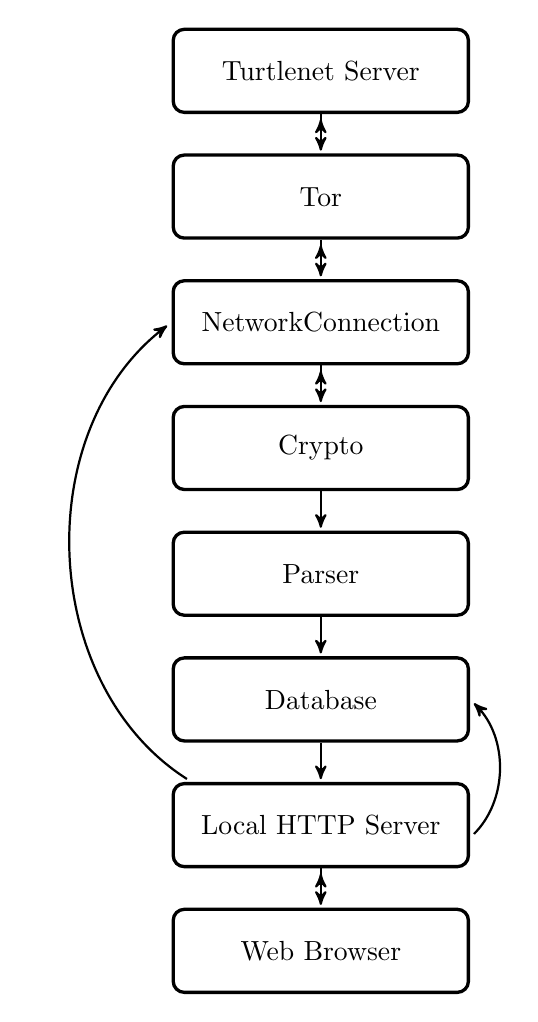
\begin{tikzpicture} [node distance=.5cm, start chain=going below,]
    \node[punktchain, join] (serv)  {Turtlenet Server};
    \node[punktchain, join] (tor)   {Tor}
        edge[pil] (serv.south);
    \node[punktchain, join] (netc)  {NetworkConnection}
        edge[pil] (tor.south);
    \node[punktchain, join] (crypt) {Crypto}
        edge[pil] (netc.south);
    \node[punktchain, join] (parse) {Parser};
    \node[punktchain, join] (db)    {Database};
    \node[punktchain, join] (gserv) {Local HTTP Server}
            edge[pil,bend left=55] (netc.west)
            edge[pil,bend right=45] (db.east);
    \node[punktchain, join] (brows) {Web Browser}
            edge[pil] (gserv.south);
\end{tikzpicture}
\label{module_diagram}
\caption{Module Interaction}
\end{figure}



\chapter{Data Flow Diagram}
\begin{figure}[h]
\centering
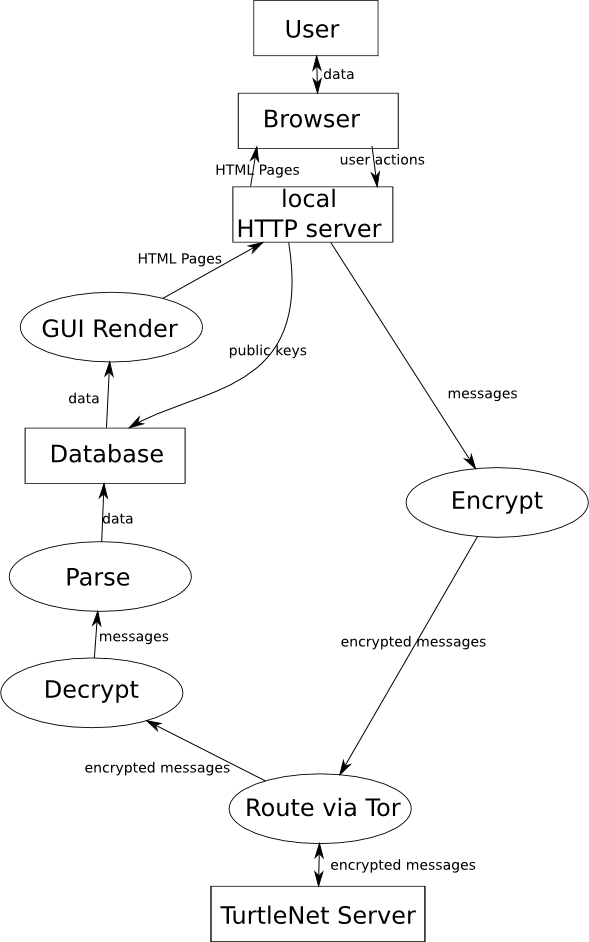
\includegraphics[width=0.8\textwidth]{images/design/data_flow_diagram.png}
\label{data_flow}
\caption{Data Flow Diagram}
\end{figure}


\chapter{Use Case Diagrams}
Here we have a use case diagram displaying an actors interaction with our 
system. It shows the functionality available to both the client, and the 
operator. We also have a sequence diagram to augment the use case diagrams.

%\begin{landscape}

\begin{tikzpicture}

%Actor Declaration
\umlactor[x=0,y=8]{Client}

\begin{umlsystem}[x=4,y=0]{System}
%Client Use case Declarations

%Public Key Use Cases
\umlusecase[name=ucPublicKey,x=0,y=4]{Manage Relations}
\umlusecase[name=ucAddAuthorise,x=5,y=3]{Add/Authorise}
\umlusecase[name=ucAddPublicKey,x=10,y=3]{Public Key}
\umlusecase[name=ucQrCode,x=10,y=2]{QR Code}
\umlusecase[name=ucCategorise,x=5,y=4]{Categorise}
\umlusecase[name=ucIgnore,x=5,y=5]{Ignore}

%Account Use Cases
\umlusecase[name=ucAccount,x=0,y=7]{Account Management}
\umlusecase[name=ucCreateClaim,x=5,y=6]{Create/Claim}
\umlusecase[name=ucPDATA,x=5,y=7]{Profile Data}
\umlusecase[name=ucDataAdd,x=10,y=6]{Add Profile Data}
\umlusecase[name=ucDataEditUpdate,x=10,y=7]{Edit/Update}

%Communication Use Cases
\umlusecase[name=ucCommunication,x=0,y=10.5]{Communication}
\umlusecase[name=ucEncrypt,x=5,y=8]{Encrypt}
\umlusecase[name=ucDecrypt,x=2,y=8]{Decrypt}
\umlusecase[name=ucRtChat,x=5,y=9]{Real-Time Chat}
\umlusecase[name=ucPost,x=5,y=10]{Post}
\umlusecase[name=ucPostOwnWall,x=10,y=9]{Own Wall}
\umlusecase[name=ucPostOtherWall,x=10,y=10]{Other's Wall}
\umlusecase[name=ucComment,x=5,y=11]{Comment}
\umlusecase[name=ucLike,x=5,y=12]{Like}
\umlusecase[name=ucUpdateDb,x=5,y=13]{Event}

%Revoke Use Case
\umlusecase[name=ucRevoke,x=0,y=14]{Revoke Private Key}

\end{umlsystem}

%Start of Client's Relations

%Public Key Relations
\umlassoc[name=assClientPublicKey]{Client}{ucPublicKey}
\umlextend[name=extPublicAdd]{ucAddAuthorise}{ucPublicKey}
\umlextend[name=extPublicCategorise]{ucCategorise}{ucPublicKey}
\umlextend[name=extPublicIgnore]{ucIgnore}{ucPublicKey}
\umlextend[name=extPublicAddKey]{ucAddPublicKey}{ucAddAuthorise}
\umlextend[name=extPublicAddQr]{ucQrCode}{ucAddAuthorise}

%Account Relations
\umlassoc[name=assClientAccount]{Client}{ucAccount}
\umlextend[name=extAccountCreateClaim]{ucCreateClaim}{ucAccount}
\umlextend[name=extAccountPDATA]{ucPDATA}{ucAccount}
\umlextend[name=extAccountDataAdd]{ucDataAdd}{ucPDATA}
\umlextend[name=extAccountDataEdit]{ucDataEditUpdate}{ucPDATA}

%Communication Relations
\umlassoc[name=assClientCommunication]{Client}{ucCommunication}
\umlinclude[name=extCommunicationEncrypt]{ucEncrypt}{ucCommunication}
\umlinclude[name=extCommunicationEncrypt]{ucDecrypt}{ucCommunication}
\umlextend[name=extCommunicationRtChat]{ucRtChat}{ucCommunication}
\umlextend[name=extCommunicationPost]{ucPost}{ucCommunication}
\umlextend[name=extPostOwnWall]{ucPostOwnWall}{ucPost}
\umlextend[name=extPostOtherWall]{ucPostOtherWall}{ucPost}
\umlextend[name=extComment]{ucComment}{ucCommunication}
\umlextend[name=extLike]{ucLike}{ucCommunication}
\umlextend[name=extUpdateDb]{ucUpdateDb}{ucCommunication}

%Private Key Relation
\umlassoc[name=assClientRevoke]{Client}{ucRevoke}

\end{tikzpicture}

\begin{tikzpicture}

%Actor Declaration
\umlactor[x=4,y=2.5]{Server Operator}

\begin{umlsystem}[x=0,y=0]{System}
%Start of Server OP's use cases

%Server Status use Cases
\umlusecase[name=ucServerStatus,x=0,y=0]{Server Status}
\umlusecase[name=ucServerStart,x=-5,y=0]{Start}
\umlusecase[name=ucServerStop,x=-5,y=1]{Stop}
\umlusecase[name=ucServerLoad,x=-9,y=1]{Monitor Server Load}

%Check Use Cases
\umlusecase[name=ucCheck,x=0,y=2]{Inspect}
\umlusecase[name=ucClientIP,x=-5,y=2]{Client IP}
\umlusecase[name=ucJoinTime,x=-10,y=2]{Login Times}
\umlusecase[name=ucMessagesSent,x=-5,y=3]{Messages}

%Deletion Use Cases
\umlusecase[name=ucDeleteMessage,x=0,y=5]{Delete Message}
\umlusecase[name=ucSpecificMessage,x=-5,y=4]{Specific Message}
\umlusecase[name=ucTimeBased,x=-5,y=5]{Time Based}
\umlusecase[name=ucAll,x=-5,y=6]{All}
\umlusecase[name=ucByIp,x=-10,y=5]{By IP}

%Server Status Relations

%Status Relations
\umlassoc[name=assOpStatus]{Server Operator}{ucServerStatus}
\umlextend[name=extStatusStart]{ucServerStart}{ucServerStatus}
\umlextend[name=extStatusStop]{ucServerStop}{ucServerStatus}
\umlextend[name=extStatusLoad]{ucServerLoad}{ucServerStatus}

%Check Relations
\umlassoc[name=assOpStatus]{Server Operator}{ucCheck}
\umlextend[name=extCheckIP]{ucClientIP}{ucCheck}
\umlextend[name=extJoinTime]{ucJoinTime}{ucClientIP}
\umlextend[name=extMessagesSent]{ucMessagesSent}{ucCheck}

%Deletion Relations
\umlassoc[name=assDelete]{Server Operator}{ucDeleteMessage}
\umlextend[name=extSpecific]{ucSpecificMessage}{ucDeleteMessage}
\umlextend[name=extTimeBased]{ucTimeBased}{ucDeleteMessage}
\umlextend[name=extAll]{ucAll}{ucDeleteMessage}
\umlextend[name=extIpTimeBased]{ucByIp}{ucTimeBased}
\umlextend[name=extIpAll]{ucByIp}{ucAll}

\end{umlsystem}

\end{tikzpicture}

%\end{landscape}

\begin{figure}[h]
    \centering
    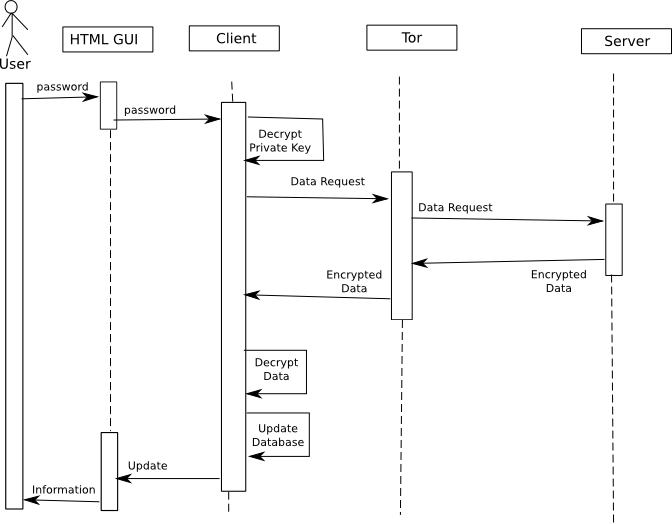
\includegraphics[width=\textwidth]{images/design/sequence_recieve.png}
    \caption{Sequence Diagram}
    \label{fig:sequence}
\end{figure}


\chapter{Protocol}
\section{High Level Summary of Protocol}
\todo[noline]{pretty dataflow diagrams}
\textbf{Creating an account} is done by generating an RSA keypair, and choosing
a name. An unencrypted (but signed) message is then posted to the server
associating that keypair with that name. In this way, by knowing the public key
of someone, you may discover their name in the service, but not vice versa.\\

\textbf{Connecting for the first time} Every unencrypted message stored on the
server is downloaded(signed nicknames and nothing more). At this time the local
database contains only signed messages claiming usernames. The public keys are 
not provided, these are of use only when you learn the public key behind a name. 
The rationale for not providing public keys is provided in the section regarding 
adding a friend. Messages posted after your name was claimed will require 
downloading too, as once you claim a name people may send you messages. It's 
worth noting that messages from before you connected for the first time are now 
downloaded because they can not have been sent to you (with a compliment client) 
if someone retroactively grants you permission to view something they publish it 
as a new message with an old timestamp; the sole exception to this is when you 
connect using a new device, in which case all messages since you first claimed a 
name will be downloaded.\\

\textbf{Connecting subsequently} The client requests every message stored on the
server since the last time they connected up to the present. Decryptable
messages are used to update the local DB, others are discarded.\\

\textbf{Continued connection} During a session the client requests updates from
the server every 0.5-5 seconds (configurable by the user).\\

\textbf{Adding a friend} is performed by having a friend email (or otherwise
transfer) you their public key. This is input to the client, and it finds their
username (via public posting that occurred when registering). You may now
interact with that person. They may not interact with you until they receive
your public key. Public key transferral will be performed via exchanging plaintext
base64 encoded strings, or QR codes. The user will be prompted, after retrieving
the username of the user, to categorise them.\\

\textbf{Talking with a friend or posting on your wall} is achieved by writing
a message, signing it with your private key, and encrypting one copy of it with
each of the recipients public keys before posting it to the server. The client
prevents one from posting a message to someone's public key if they have not
claimed a nickname.\\

\textbf{Posting to a friends wall, commenting and liking} may be requested by
sending a EPOST/CMNT/LIKE message to the friend (upon whose wall/post you are
posting, commenting or liking), when that friend logs in they will receive your
request, and may confirm or deny it. If they confirm then they take your (signed)
message and transmit it to each of their friends as previously described. Given
that authentication is entirely based on crypto signatures it doesn't matter
that your friend relays the message.This is required because it is impossible
for one to know who is able to see the persons wall, post, or comment upon which
you seek to post, like, or comment.





\chapter{Class Interfaces}
\section{Class Interfaces}
The following is a description of the public functions of all public classes.
Many classes have inner private classes they use for convenience, however to
simplify interaction between parts of our system ('modules') we have very few
convenience classes.

\todo{Reconcile return types with stated public classes}
\todo{specify what's static}

\begin{table}[h]
    \centering
    \begin{tabular}{p{1cm}p{1cm}p{3cm}}
    return & function & description\\ \hline
    void   & main() & (static) starts the server\\
    \end{tabular}
    \caption{Server}
\end{table}

\begin{table}[h]
    \centering
    \begin{tabular}{p{1cm}p{1cm}p{9cm}}
    return & function & description\\ \hline
    void   & main()   & (static) constructs and starts all necessary classes and threads, runs the main loop\\
    \end{tabular}
    \caption{Client}
\end{table}

\begin{table}[h]
    \centering
    \begin{tabular}{p{1cm}p{2.8cm}p{9cm}}
    return   & function            & description\\ \hline
    N/A      & NetworkConnection() & Constructs a NetworkConnection and connects to the given URL (through tor)\\
    void     & run()               & periodically download new messages until asked to close, downloaded messages are stored in a FIFO buffer\\
    void     & close()             & kills the thread started by run()\\
    boolean  & hasMessage()        & return true if there is a message in the buffer, false otherwise\\
    String   & getMessage()        & return the oldest message in the buffer\\
    
    boolean  & claimName()     & claim a given username, returns true on success, false otherwise\\
    void     & revokeKeypair() & revokes your keypair\\
    void     & pdata()         & adds or updates profile information\\
    void     & chat()          & begins or continues a conversation\\
    void     & post()          & post a message to your wall\\
    void     & fpost()         & post a message to a friends wall\\
    void     & comment()       & comment on a comment or post\\
    void     & like()          & like a comment or post\\
    void     & event()         & create an event\\
    void     & revoke()        & revoke your keypair\\
    \end{tabular}
    \caption{NetworkConnection}
\end{table}

\begin{table}[h]
    \centering
    \begin{tabular}{p{1.4cm}p{3.3cm}p{9cm}}
    return     & function        & description\\ \hline
    boolean    & keysExist()     & (static) return true if the user has a keypair, false otherwise\\
    void       & keyGen()        & (static) generate a keypair for the user\\
    PublicKey  & getPublicKey()  & (static) returns the users public key\\
    PrivateKey & getPrivateKey() & (static) returns the users private key\\

    String     & sign()      & (static) returns an RSA signature of the passed string\\
    boolean    & verifySig() & (static) returns true if author signed msg, false otherwise\\
    String     & encrypt()   & (static) returns an encrypted message constructed from the passed parameters\\
    Message    & decrypt()   & (static) decrypts the passed string, returns the appropriate message, on failure a NULL message is returned\\
    String    & base64Encode() & (static) base64 encodes the passed data, returns the string\\
    byte[]    & base64Decode() & (static) base64 decodes the passed data, returns the byte[]\\
    String    & encodeKey()    & (static) encodes a public key as a string, returns that string (X509)\\
    PublicKey & decodeKey()    & (static) decodes a public key encoded as a string, returns that public key(X509)\\
    String    & hash ()        & (static) returns the SHA256 hash the the passed string as a hex string\\
    int       & rand ()        & (static) returns a pseudorandom value <= max and >= min\\
    \end{tabular}
    \caption{Crypto}
\end{table}

\begin{table}[h]
    \centering
    \begin{tabular}{p{1cm}p{2.6cm}p{9cm}}
    return & function & description\\ \hline
    void   & parse()  & (static) parses a sting message, records parsed data in the database\\
    \end{tabular}
    \caption{Parser}
\end{table}

\todo{go over DB interface with GUI guys and Aishah}
\begin{table}[h]
    \centering
    \begin{tabular}{p{3cm}p{3cm}p{9cm}}
    return                & function       & description\\ \hline
    
    void                  & addClaim()     & adds a username CLAIM message\\
    pair<string,string>[] & getClaims()    & gets all CLAIMs to usernames\\
    string[]              & getUsernames() & gets all usernames\\
    
    void                    & addRevocation()  & adds a keypair revocation\\
    pair<PublicKey, long>[] & getRevocations() & gets all revocations\\
    boolean                 & isRevoked()      & returns the time a key was revoked, if the given key has not been revokes then 0 is returned.\\
    
    void   & addPData() & adds (or amends existing) profile data\\
    string & getPData() & gets the specified piece of profile data for a specified user\\
    
    void                  & createChat() & creates new chat\\
    pair<string,string>[] & getChat()    & returns messages from a given chat\\
    void                  & addToChat()  & adds a post to a given chat\\
    
    void                  & addPost()  & creates new post, on your or another's wall\\
    pair<string,string>[] & getPosts() & gets all posts either within timeframe, or from certain people within a timeframe\\
    
    void                  &  addComment() & adds a comment onto post or comment\\
    pair<string,string>[] & getComments() & gets all comments for a post or comment\\
    
    void     & addLike() & likes a post or comment\\
    String[] & getLikes() & gets all likes from certain person within a timeframe\\
    int      & countLikes() & gets the number of likes for a comment or post\\
    
    void                & addEvent()     & adds new event\\
    pair<string,long>[] & getEvent()     & gets all events within timeframe\\
    void                & acceptEvent()  & accepts notification of an event\\
    void                & declineEvent() & declines notification of an event\\
    
    void        & addKey()  & adds a public key to the DB\\
    PublicKey[] & getKey()  & gets the public key for a usernamne, or all which are stored)\\
    string      & getName() & gets a username for the given public key\\

    void & addFriend()     & adds the given friend to the DB\\
    void & addCategory()   & adds a new category to the DB\\
    void & addToCategory() & adds a user to a category\\
    \end{tabular}
    \caption{Database}
\end{table}

\begin{table}[h]
    \centering
    \begin{tabular}{p{1cm}p{2.6cm}p{9cm}}
    return  & function    & description\\ \hline
    N/A     & GUI()       & Constructs a GUI\\
    void    & run()       & continually updates the GUI from the DB\\
    void    & close()     & kills the GUIServer thread\\
    boolean & isRunning() & returns true if the GUIServer is running, false otherwise\\
    \end{tabular}
    \caption{GUI}
\end{table}

\begin{table}[h]
    \centering
    \begin{tabular}{p{1cm}p{2.6cm}p{9cm}}
    return  & function       & description\\ \hline
    N/A     & Message()      & Constructs a message with given data\\
    
    Message & parse()        & (static) parses the string representation of a message into a message\\
    
    String  & toString()     & creates a string representation of the message\\
    String  & getCmd()       & returns the type of message\\
    String  & getContent()   & returns the content of the message\\
    String  & getSig()       & returns the RSA signature on the message\\
    long    & getTimestamp() & returns the timestamp on the message\\
    \end{tabular}
    \caption{Message}
\end{table}

\begin{table}[h]
    \centering
    \begin{tabular}{p{1cm}p{2cm}p{9cm}}
    return & function & description\\ \hline
    
    N/A    & Pair()   & Constructs a pair with given data\\
    A      & first()  & returns the first value passed to the constructor\\
    B      & second() & returns the second value passed to the constructor\\
    \end{tabular}
    \caption{Pair\textless A, B\textgreater }
\end{table}

\section{Class Diagram}
\missingfigure{Class Diagram Goes Here}


\chapter{Pseudocode}
\section{Server}
\begin{lstlisting}
static void main () {
    startGUIthread()
    startServer()
}
\end{lstlisting}

\begin{lstlisting}
static void start () {
    socket = new ServerSocket(port)
    while (running) {
        incoming = socket.accept()
        t = new Thread(new Session(incoming))
        t.start()
    }
    
    shutdown()
}
\end{lstlisting}

\section{Client}
\begin{lstlisting}
static void main () {
    NetworkConnection connection    = new NetworkConnection("server.tld")
    Thread            networkThread = new Thread(connection)
    Database          db            = new Database("./db")
    GUI               gui           = new GUI(db, connection)
    Thread            guiThread     = new Thread(gui)
        
    if (!Crypto.keysExist())
        Crypto.keyGen()
        
    networkThread.start()
    guiThread.start()
        
    while (gui.isRunning())
        while (connection.hasMessage())
            Parser.parse(Crypto.decrypt(connection.getMessage()), db)
}
\end{lstlisting}

\section{Crypto}
\begin{lstlisting}
keyGen () {
    keypair = generateRSAkeypair()
    pw      = GUI.getUserInputString()
    filesystem.write("keypair", Crypto.aes(pw, keypair))
}
\end{lstlisting}

\begin{lstlisting}
static String sign (String msg) {
    byte[] sig = SHA1RSAsign(msg.getBytes("UTF-8"), Crypto.getPrivateKey())
    return Crypto.Base64Encode(sig)
}
\end{lstlisting}

\begin{lstlisting}
static String encrypt(String cmd, String text, PublicKey recipient,
                      NetworkConnection connection) {
    Message msg = new Message(cmd, text, connection.getTime()+Crypto.rand(0,50),
                              Crypto.sign(text))
    
    //encrypt with random AES key with random initalization vectors
    byte[]     iv = new byte[16]
    byte[] aeskey = new byte[16]
    
    fillWithRandomData(iv);
    fillWithRandomData(aeskey);
    
    byte[] aesCipherText = aes(aeskey, iv, msg.toString().getBytes("UTF-8"))
            
    //encrypt AES key with RSA
    byte[] encryptedAESKey = rsa(Crypto.getPrivateKey(), aeskey)
            
    //"iv\RSA encrypted AES key\ciper text"
    return Base64Encode(iv) + "\\" + Base64Encode(encryptedAESKey) +
           "\\" + Base64Encode(aesCipherText)
}
\end{lstlisting}

\begin{lstlisting}
static Message decrypt(String msg) {
    //handle claim messages (which are the only plaintext in the system)
    if (msg.substring(0,2).equals("c "))
        return Message.parse(Base64Decode(msg.substring(2)))
    
    //handle encrypted messages
    String[] tokens = new String[3]
    tokens = tokenize("msg", "\")
        
    byte[] iv            = Base64Decode(tokens[0])
    byte[] cipheredKey   = Base64Decode(tokens[1])
    byte[] cipherText    = Base64Decode(tokens[2])
            
    //decrypt AES key
    byte[] aesKey = rsaDecrypt(cipheredKey, getPrivateKey())
            
    //decrypt AES Ciphertext
    aes.init(Cipher.DECRYPT_MODE, aesKeySpec, IVSpec)
    byte[] messagePlaintext = aesDecrypt(cipherText, aesKey, iv)

    return Message.parse(messagePlaintext)
}
\end{lstlisting}

\section{Database}
Most database functions are just going to construct parameterized SQL queries to
be sent to the database from passed parameter values. The exceptions which
include significant computing are listed here:

\begin{lstlisting}
void addKey (PublicKey k) {
    for each row r in table message_claim
        if (Crypto.verifySig(r.signature, k))
            addFriend(new Friend(k, r.username))
}
\end{lstlisting}

\begin{lstlisting}
PublicKey[] getKey (String username) {
    PublicKey[] keys
    for each row r in table user
        if (r.username == username)
            keys.add(r.public_key)
    return keys
}
\end{lstlisting}

\begin{lstlisting}
void addToCategory (Friend f, String category) {
    for each row r in table wall_post
        if (r.permission_to includes category)
            sendMessage(r, f)
}
\end{lstlisting}


\section{Network Connection}
The vasy majority of messages here merely construct the appropriate message from
the parameters and pass it to serverCmd()

\begin{lstlisting}
void main (String _url) {
    url = _url
    messages    = new Vector<String>()
    messageLock = new Semaphore(1)
    connected   = true
    
    File lastReadFile = new File("./db/lastread")
    lastRead = Long.parseLong(lastReadFile.readLine())
}
\end{lstlisting}

\begin{lstlisting}
void run () {
    while(running) {
        sleep(delay)
        downloadNewMessages()
    }
}
\end{lstlisting}

\begin{lstlisting}
String[] serverCmd(String cmd) {
    Socket s;
    BufferedReader in;
    PrintWriter out;
        
        
    //connect
    s = new Socket(new Proxy(Proxy.Type.SOCKS, new InetSocketAddress("localhost", 9050)))
    s.connect(new InetSocketAddress(url, port))
    in  = new BufferedReader(new InputStreamReader(s.getInputStream()))
    out = new PrintWriter(s.getOutputStream(), true)
        
    //send command
    out.println(cmd);
    out.flush();
        
    //recieve output of server
    Vector<String> output = new Vector<String>();
    String line = null;
    do {
        line = in.readLine();
        if (line != null)
            output.add(line);
    } while (line != null);
}
\end{lstlisting}

\section{Parser}
\begin{lstlisting}
void parse (String msg, Database db) {
    Message m = Message.parse(msg)
    if (m.cmd == "PDATA") {
        String[] tokens = tokenize(msg.content, ":")
        db.addPData(tokens[0], tokens[1])
    } else if (m.cmd == "REVOKE") {
        PublicKey key
        for row r in table users
            if Crypto.verifySig(r.public_key, m.signature)
                key = r.public_key
        db.addRevocation(key)
    } else if {
        etc...
}
\end{lstlisting}


\chapter{Database}
\section{Database design description}
{\it Note the difference between 'main user' and 'user'. Main user refers to the 
user who owns the local database. 'User' or 'other user' refers to other users, 
usually the relations of the main user.}

\subsection{user table} 
This table stores user details, which includes the main user's own details and 
its relations. As the user makes a new relation with another user, its details 
will be stored in this table. Every user has their own public key which uniquely 
identifies their accounts which also be stored in this table.

\subsection{user, is\_in\_category, category table}
With the category table, the user can create new categories to group his 
relations. As it is possible for many users to belong in many categories, the 
{\it is\_in\_category} table is needed to identify which set of users belong in 
the categories.

\subsection{user, is\_invited, events table}
These tables suggest that users can create events. One particular feature 
regarding these tables that on the {\it is\_invited table}, where the user (the 
main one) can invite anyone individually from the relations list or as a group 
from the category list. However, there will be no tuples added under this table 
when another user posts the event. Reason being is that the main user is not 
allowed to see who the list of other users invited in the event which was not 
created by the main user. 

When the main user creates an event, he invites other people, either from the 
user table or from the category table or both. Once the invitation is sent out 
to those users, the users can either accept or reject the invitation. Using the 
{\it decision} attribute from the {\it is\_invited} table, if decision has not 
been made, it will be NULL. If user accepts the invitation, it will be 1 for 
true. If rejected, it will be 0 for false. 

\subsection{user, allowed\_to, wall\_post table}
When users create post, its data will be inserted into the {\it wall\_post} 
table. The attribute {\it from} refers to the user who has created the post, 
whilst the attribute {\it to} refers to the user who is referred or mentioned 
in this post. The main user can also choose a allow a set of his relations to 
view his post. Using the {\it allowed\_to} table, similar as the 
{\it is\_invited} table, the main user can select his relations either 
individually or through categories or both. If the post is created by another 
user, no tuples will be inserted into the {\it allowed\_to} table.

\subsection{user, has\_like, wall\_post table}
Users can like any posts that appears in his main wall or personal wall. When a 
post is liked, a new tuple is created in the has\_like table to identify who 
liked the post, which post is liked, and the time the post is liked. These likes 
are counted and displayed in the GUI showing how many users have liked this post.

\subsection{user, has\_like, has\_comment table}
Other than liking posts, users can like individual comments as well. Same 
feature as liking the post by this time, data is inserted into the attribute 
{\it comment\_id} from the {\it has\_like} table to show which particular comment 
has been liked by this user.

\subsection{user, has\_comment, wall\_post table}
Users can comment on posts. When post is commented on, a new tuple will be added 
into the {\it has\_comment} table on information like the content of the comment, 
which post has been commented on, who commented on the post, and the time of 
comment.

\subsection{user, has\_comment table}
Users can also comment on comments itself. This will create and indentation on 
the GUI to suggest that the parent comment has a child comment. When a comment is 
commented upon, the attribute {\it comment\_comment\_id} will insert the parent 
comment\_id which shows the relation of two comments, one parent and the other 
being the child.

\subsection{user, is\_in\_message, private\_message table}
Another functionality found in Turtlenet is the user is able to send private 
messages to users. When a private message is created by the main user, a new 
tuple is added into the {\it private\_message} table. The user then has the 
option to add other user(s) into the conversation. When done so, a tuple or 
tuples, depending on the number of users he has added onto the conversation, are 
added into the {\it is\_in\_message} table. This inserts the information such as 
the time of when the user has been added into the conversation, the user's ID 
and message ID. The {\it private\_message} table on the other hand stores data 
such as the content of the message and the time for which this whole conversation 
was created. 

\subsection{message\_claim table}
When the main user has not required any public key from the other user he is 
intended to add, the details will be entered onto this table until which a pubic 
key is retrieved. When retrieved, this information found in this table will be 
deleted and transferred into the {\it user} table along with other information 
that comes with it.

\subsection{key\_revoke table}
In times when malicious activity might have been conducted, the users of 
Turtlenet is able to revoke their relations signature key. A signature suggests 
that this post is written by this person in particular, so when it is revoked, 
whatever that has been posted with this signature is considered false. This will 
inform the user not to trust any information that has been posted with this 
signature in particular. 

\subsection{login\_logout\_log table}
This table simply tracks the login and logout activities of the main user. When a 
user logs in and out, a new tuple will be inserted into this table.

\clearpage

\section{Table layout of the database}
NB: Public keys are 217 characters long, all id's are auto-incremented.

\begin{table}[!ht]
\caption{user}
\centering
\begin{tabular}{c c c}
\hline\hline
Name               & Datatype    & Key \\
\hline
user\_id           & INT          & PK \\  % 64-bit has key public key
username           & VARCHAR(25)  &    \\
name               & VARCHAR(30)  &    \\
birthday           & DATE         &    \\
sex                & VARCHAR(1)   &    \\
email              & VARCHAR(30)  &    \\
public\_key        & VARCHAR(600)   & PK \\
\hline
\end{tabular}
\label{table:nonlin}
\end{table}

\begin{table}[!ht]
\caption{is\_in\_category}
\centering
\begin{tabular}{c c c}
\hline\hline
Name               & Datatype    & Key \\
\hline
is\_in\_id         & INT     & PK   \\
category\_id       & INT     & FK   \\
user\_id           & INT     & FK   \\
\hline
\end{tabular}
\label{table:nonlin}
\end{table}

\begin{table}[!ht]
\caption{category}
\centering
\begin{tabular}{c c c}
\hline\hline
Name               & Datatype    & Key \\
\hline
category\_id       & INT         & PK  \\
name               & VARCHAR(30) &     \\
\hline
\end{tabular}
\label{table:nonlin}
\end{table}


\begin{table}[!ht]
\caption{private\_message}
\centering
\begin{tabular}{c c c}
\hline\hline
Name               & Datatype    & Key \\
\hline
message\_id        & INT         & PK  \\
from               & INT         &     \\
content            & VARCHAR(50) &     \\
time               & DATE        &     \\
\hline
\end{tabular}
\label{table:nonlin}
\end{table}

\begin{table}[!ht]
\caption{is\_in\_message}
\centering
\begin{tabular}{c c c}
\hline\hline
Name               & Datatype        & Key \\
\hline
is\_in\_id         & INT             & PK  \\
time               & DATETIME        &     \\
message\_id        & INT             & FK  \\
user\_id           & INT             & FK  \\
\hline
\end{tabular}
\label{table:nonlin}
\end{table}

\begin{table}[!ht]
\caption{wall\_post}
\centering
\begin{tabular}{c c c}
\hline\hline
Name                    & Datatype    & Key \\
\hline
wall\_id                & INT         & PK  \\
from                    & INT         & FK  \\
to                      & INT         & FK  \\
content                 & VARCHAR(50) &     \\
time                    & DATETIME    &     \\
\hline
\end{tabular}
\label{table:nonlin}
\end{table}

\begin{table}[!ht]
\caption{allowed\_to}
\centering
\begin{tabular}{c c c}
\hline\hline
Name                    & Datatype    & Key \\
\hline
allowed\_to\_id         & INT         & PK  \\
user\_id                & INT         & FK  \\
category\_id            & INT         & FK  \\
post\_id                & INT         & FK  \\
\hline
\end{tabular}
\label{table:nonlin}
\end{table}

\begin{table}[!ht]
\caption{has\_comment}
\centering
\begin{tabular}{c c c}
\hline\hline
Name                 & Datatype     & Key \\
\hline
comment\_id          & INT(100)     & PK  \\
comment\_content     & VARCHAR(50)  &     \\
post\_id             & INT(100)     & FK  \\
user\_id             & VARCHAR(50)  & FK  \\
comment\_comment\_id & INT(100)     & FK   \\
time                 & DATETIME     &     \\
\hline
\end{tabular}
\label{table:nonlin}
\end{table}

\begin{table}[!ht]
\caption{has\_like}
\centering
\begin{tabular}{c c c}
\hline\hline
Name               & Datatype    & Key \\
\hline
like\_id           & INT          & PK  \\
post\_id           & INT          & FK  \\
user\_id           & INT          & FK  \\
comment\_id        & INT          & FK  \\
time               & DATETIME     &     \\
\hline
\end{tabular}
\label{table:nonlin}
\end{table}

\begin{table}[!ht]
\caption{events}
\centering
\begin{tabular}{c c c}
\hline\hline
Name                    & Datatype    & Key \\
\hline
event\_id               & INT          & PK  \\
title                   & VARCHAR(10)  &     \\
content                 & VARCHAR(40)  &     \\
time                    & DATETIME     & \\
start\_date             & DATETIME     & \\
end\_date               & DATETIME     & \\
from                    & INT          & FK  \\
\hline
\end{tabular}
\label{table:nonlin}
\end{table}

\begin{table}[!ht]
\caption{is\_invited}
\centering
\begin{tabular}{c c c}
\hline\hline
Name                    & Datatype    & Key \\
\hline
is\_invited\_id         & INT         & PK  \\
user\_id                & INT         & FK  \\
is\_in\_category\_id    & INT         & FK  \\
event\_id               & INT         & FK  \\
decision                & BIT         &     \\
\hline
\end{tabular}
\label{table:nonlin}
\end{table}

\begin{table}[!ht]
\caption{login\_logout\_log}
\centering
\begin{tabular}{c c c}
\hline\hline
Name               & Datatype    & Key \\
\hline
log\_id            & INT         & PK  \\
login\_time        & DATETIME    &     \\
logout\_time       & DATETIME    &     \\
\hline
\end{tabular}
\label{table:nonlin}
\end{table}

\begin{table}[!ht]
\caption{key\_revoke}
\centering
\begin{tabular}{c c c}
\hline\hline
Name               & Datatype    & Key \\
\hline
revoke\_id         & INT          & PK  \\
signature          & VARCHAR(45)  &     \\
time               & DATETIME     &     \\
\hline
\end{tabular}
\label{table:nonlin}
\end{table}

\begin{table}[!ht]
\caption{message\_claim}
\centering
\begin{tabular}{c c c}
\hline\hline
Name               & Datatype    & Key \\
\hline
username           & VARCHAR(25) & PK  \\
signature          & VARCHAR(45) &     \\
\hline
\end{tabular}
\label{table:nonlin}
\end{table}

\clearpage

\begin{landscape}
\begin{figure}[h]
    
    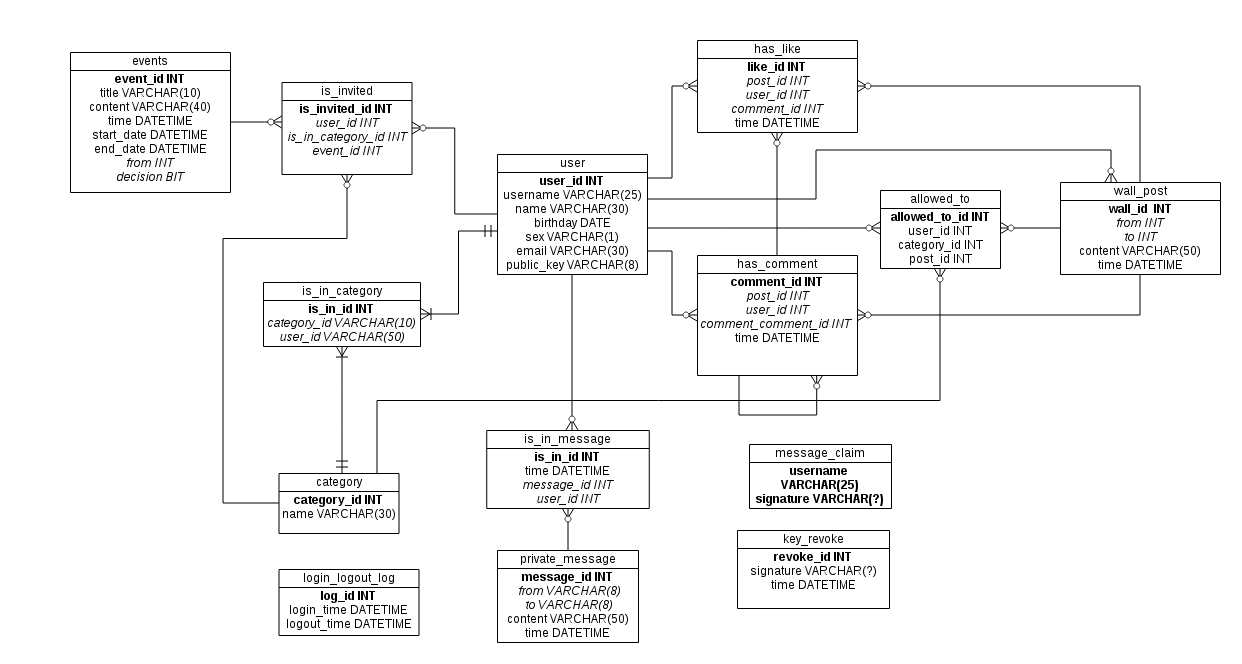
\includegraphics[width=1.4\textwidth]{images/design/project_er_diagram.png}
    \caption{Database Entity Relationship diagram}
    \label{fig:db_er_diag}
\end{figure}
\end{landscape}

\chapter{Transaction details}
The table below shows the transaction details of each function which will be found in the program. There are four types of transactions for databases which are insert, read, update and delete. 

Insertion is done when new data is added into a NULL attribute.
Read on the other hand, is to view information from selected table(s) and its attribute(s).
Similar as insertion but update is conducted when data already exists in the particular attribute. This basically removes previous data and add a new one.
Lastly, delete, as it is self explanatory, deletes the whole tuple from the database. However this is usually avoided in database norms.

\begin{center}
    \begin{tabular}{ | p{3cm} | p{5cm} | p{3cm} |}
    \hline
    {\bf Function}        & {\bf Table(s) involved} & {\bf Transaction(s)} \\ \hline
    addClaim()      &                   &                \\ \hline 
    getClaims       &                   &                \\ \hline 
    getUsernames    & user              & Read           \\ \hline 
    addRevocation   & key\_revoke       & Insert         \\ \hline 
    getRevocations  & key\_revoke       &    Read        \\ \hline 
    isRevoked()     & key\_revoke       &  Insert        \\ \hline 
    addPData()      &                   &                \\ \hline 
    getPData()      &                   &                \\ \hline 
    createChat()    & private\_message  &  Insert        \\ \hline 
    getChat()       & private\_message, is\_in\_message             & Read           \\ \hline 
    addToChat()     & is\_in\_message   &   Insert       \\ \hline 
    addPost()       & wall\_post        &  Insert        \\ \hline 
    getPosts()      & wall\_post        &    Read        \\ \hline 
    \end{tabular}
\end{center}

\begin{center}
    \begin{tabular}{ | p{3cm} | p{5cm} | p{3cm} |}
    \hline
    {\bf Function}        & {\bf Table(s) involved} & {\bf Transaction(s)} \\ \hline
    addComment()    & has\_comment      &   Insert       \\ \hline 
    getComments()   & has\_comment      &  Read          \\ \hline 
    addLike()       & has\_like         &  Insert        \\ \hline 
    getLikes()      & has\_like         &  Read          \\ \hline 
    countLikes()    & has\_like         &  Read and count\\ \hline 
    addEvent()      & events            &    Insert      \\ \hline 
    getEvent()      & events            &  Read          \\ \hline 
    acceptEvent()   & events            &   Update       \\ \hline 
    declineEvent()  & events            &  Update        \\ \hline 
    addKey()        &                   &                \\ \hline 
    getKey()        &                   &                \\ \hline 
    getName()       & user              &  Read          \\ \hline 
    addFriend()     &                   &                \\ \hline 
    addCategory()   & category          &     Insert     \\ \hline  
    addToCategory() & is\_in\_category  &   Insert       \\ \hline 

    \end{tabular}
\end{center}


\chapter{User Interfaces}
As a social network, the user interface design is of high importance, as a lot 
of users of the program will have little core system knowledge, and rely 
entirely on the user interface. As a result we have looked at a variety of 
options into designing which will be the best for the project.

\section{Swing}
Swing is the primary Java GUI toolkit, providing a basic standpoint for entry 
level interface designing. Introduced back in 1996, Swing was designed to be 
an interface style that required minimal changes to the applications code, 
providing the user with a pluggable look and feel mechanism. It has been apart 
of the standard java library for over a decade, which, as I will now explain, 
may not be to our benefit.

Swing, whilst an excellent language to begin with, and write simple applications
in, is quite dated. As our group advisor put it when inquiring about what we 
would be coding the user interface in:

\begin{quote}
"You should avoid Swing to prevent it looking like it was done in the 
seventies." - Sebastian Coope
\end{quote}

Sebastian is not wrong either, as Swing does a very plain feel to it. "Fig ???" 
shows an old instant messaging system written with Swing by one of our team 
members. As you can see it is unlikely to appeal to the mass market with such 
visually plain appearance. This makes Swing, unlikely to be our GUI toolkit of 
choice, despite some of our members experience with it.

\section{Abstract Window Toolkit}
Abstract Window Toolkit (otherwise known as AWT), was another choice given 
that we are programming in Java, and synchronicity between the two would be an 
advantage. Whilst AWT retained some advantages such as its style blending in 
with each operating system it runs on, it is even older than Swing being Java's 
original toolkit, as per such making it redundant for this project.

\section{Standard Widget Toolkit}
Standard Widget Toolkit (otherwise known as SWT), is one of the more promising 
candidates so far given its look and up-to-date support packages. The latest 
stable release of SWT was only last year, and is capable of producing programs 
with a modern and professionally built appearance, as shown in "Fig ???".

Unlike both Swing and AWT, SWT is not provided by Sun Microsystems as a part of 
the Java platform. It is now provided and maintained by the Eclipse Foundation, 
and provided as a part of their widely used Eclipse IDE, something a lot of the 
team is familiar with.

\section{GWT}
GWT allows you to create HTML/Javascript based user interfaces for Java 
applications running locally. The interface is programmed in Java and then GWT 
creates valid HTML/Javascript automatically. A web server is required in order
for Javascript events to be sent to the Java application.

The user can then interact with the system by pointing their web browser at 
localhost. This has the benefit of being familiar to novice users as most modern 
computer interaction is done within a web browser. 

Another advantage of using GWT is the ability to alter the appearance of web 
pages using CSS. This facilitates the creation of a modern, attractive user 
interface that integrates nicely with current operating systems and software.

\section{Javascript}
It is possible to create the entire client application in Javascript and use a 
HTML/Javascript GUI. This approach removes the need for a local web server 
meaning the only software the user is required to run is a modern web browser.

Another advantage would be tight integration between the logic and interface 
elements of the client application and no risk of errors caused by using 
multiple programming languages.

The main disadvantage of this approach is the difficulty in implementing the 
required security measures and encryption in Javascript. This can be remedied by 
using a Javascript library such as the Forge project which implements many 
cryptography methods.

\begin{comment}
Starts to get more into client side logic here but I think it is important to 
mention as this method would require an entire rewrite of the client. -Louis-
\end{comment}

\chapter{Business Rules}
In standard projects the business model can commonly outline certain validation 
practices for the program or project in the form of business rules or policies. 
Our project, and its fundamental idea, works a little different than most 
projects in terms of business, as per such we have only one business rule.

\begin{quote}
\centering
\textit{"To ensure the client never sends identifying data to the server or its 
operators."}
\end{quote}

This is to ensure that the privacy of communication is always within the hands 
of the client and user, as opposed to any who run the network. To violate this 
single rule would be going against both the company ideals, and the projects 
goals.


%\chapter{QR}
%I've found a website that generates QR Codes - both professionally and otherwise
for free.  We could implement it into our prgram by having the program output
the URL it gives you as because it's generated via URL, we should be able to
store it in a string and then output either that or have an image viewer in the
program to output the actual image, whichever is easiest for the user.

The website's create function: http://goqr.me/api/doc/create-qr-code/
The website's read function: http://goqr.me/api/doc/read-qr-code/
A test one I did:
https://api.qrserver.com/v1/create-qr-code/?size=300x300\&data=\%3Ci'mThePublicKeyVariable\%3E\&format=svg


\chapter{Gantt Chart}
These are excerpts from the Gantt charts made during the requirements stage of
the project.  They have been used as a guide throughout the completed sections
of the project.  As the design section was foreseen as the most work-intensive
part that is encompassed within the project, particular care and attention was
made to make sure that official deadlines were met, through the use of 
un-official end dates for each task.

By doing so, therefore finishing tasks earlier than required, it has provided a 
buffer used for quality controlling the project's deliverables. A partial
reproduction of the task list is also provided:

\begin{tabular}{llrl}
    
    \toprule
    
    Task ID  & Task Description (Desc.)     & Due Date    & Deliverable       \\
    
    \midrule
    
    2        & Project Design               & 14/03/2014  & Design Segment    \\
    
    \cmidrule(r){2-3}
    2.1      & Research (Res.)              & 21/02/2014  & Research Segment  \\
    2.1.1    & Res: Database Languages      & 21/02/2014  & Same as Desc.     \\
    2.1.2    & Res: Programming Languages   & 21/02/2014  & Same as Desc.     \\
    2.1.3    & Res: Interfaces              & 21/02/2014  & Same as Desc.     \\
    \cmidrule(r){2-3}
    
    2.2      & Designs (Des.)               & 07/03/2014  & Design Segment    \\
    2.2.1    & Des: Databases               & 28/02/2014  & Same as Desc.     \\
    2.2.2    & Des: Class Interfaces        & 28/02/2014  & Same as Desc.     \\
    2.2.3    & Des: Protocol                & 28/02/2014  & Same as Desc.     \\
    2.2.4    & Des: Architecture            & 28/02/2014  & Same as Desc.     \\
    2.2.5    & Des: Sequence Diagrams       & 28/02/2014  & Same as Desc.     \\
    2.2.6    & Des: Data Flow Diagrams      & 28/02/2014  & Same as Desc.     \\
    2.2.7    & Des: Class Diagrams          & 28/02/2014  & Same as Desc.     \\
    2.2.8    & Des: Server-side Interfaces  & 28/02/2014  & Same as Desc.     \\
    2.2.9    & Des: Client-side Interfaces  & 28/02/2014  & Same as Desc.     \\
    2.2.10   & Des: Server-side Protocols   & 28/02/2014  & Same as Desc.     \\
    2.2.11   & Des: Client-side Protocols   & 28/02/2014  & Same as Desc.     \\
    2.2.12   & Des: Server-side Pseudo-code & 07/03/2014  & Same as Desc.     \\
    2.2.13   & Des: Client-side Pseudo-code & 07/03/2014  & Same as Desc.     \\
    \cmidrule(r){2-3}
    
    2.3      & Segment Review               & 10/03/2014  & Design Segment    \\
    2.3.1    & Evaluate Segment Quality     & 14/03/2014  & N/A               \\
    2.3.2    & Improve Segment              & 14/03/2014  & Design Segment    \\
    
    \bottomrule
\end{tabular}

\begin{ganttchart}{14}{12}
\addtolength{\oddsidemargin}{-1in}
\addtolength{\evensidemargin}{-1in}


    \gantttitle{February 2014}{14}                                            \\
    \gantttitlelist{15,...,28}{1}                                             \\
    \ganttgroup{Design (2)}{1}{14}                                            \\
    \ganttgroup{Research (2.1)}{1}{6}                                         \\
    \ganttbar[name=2.1.1]{2.1.1}{1}{6}                                        \\
    \ganttbar[name=2.1.2]{2.1.2}{1}{6}                                        \\
    \ganttbar[name=2.1.3]{2.1.3}{1}{6}                                        \\

    \ganttmilestone[name=msResearch]{Research}{7}                             \\
    \ganttlink{2.1.1}{msResearch}
    \ganttlink{2.1.2}{msResearch}
    \ganttlink{2.1.3}{msResearch}
    
    \ganttgroup{Design Documentation(2.1)}{9}{13}                             \\
    \ganttbar[name=2.2.1]{2.2.1}{9}{13}                                       \\
    \ganttbar[name=2.2.2]{2.2.2}{9}{13}                                       \\
    \ganttbar[name=2.2.3]{2.2.3}{9}{13}                                       \\
    \ganttbar[name=2.2.4]{2.2.4}{9}{13}                                       \\
    \ganttbar[name=2.2.5]{2.2.5}{9}{13}                                       \\
    \ganttbar[name=2.2.6]{2.2.6}{9}{13}                                       \\
    \ganttbar[name=2.2.7]{2.2.7}{9}{13}                                       \\
    \ganttbar[name=2.2.8]{2.2.8}{9}{13}                                       \\
    \ganttbar[name=2.2.9]{2.2.9}{9}{13}                                       \\
    \ganttbar[name=2.2.10]{2.2.10}{9}{13}                                     \\
    \ganttbar[name=2.2.11]{2.2.11}{9}{13}                                     \\
    \ganttbar[name=2.2.12]{2.2.12}{9}{13}                                     \\
    \ganttbar[name=2.2.13]{2.2.13}{9}{13}                                     \\
    
    \ganttlink{msResearch}{2.2.1}
    \ganttlink{msResearch}{2.2.2}
    \ganttlink{msResearch}{2.2.3}
    \ganttlink{msResearch}{2.2.4}
    \ganttlink{msResearch}{2.2.5}
    \ganttlink{msResearch}{2.2.6}
    \ganttlink{msResearch}{2.2.7}
    \ganttlink{msResearch}{2.2.8}
    \ganttlink{msResearch}{2.2.9}
    \ganttlink{msResearch}{2.2.10}
    \ganttlink{msResearch}{2.2.11}
    \ganttlink{msResearch}{2.2.12}
    \ganttlink{msResearch}{2.2.13}
    
    \ganttmilestone[name=msDesign]{Design Docs}{14}
    
    \ganttlink{2.2.1}{msDesign}
    \ganttlink{2.2.2}{msDesign}
    \ganttlink{2.2.3}{msDesign}
    \ganttlink{2.2.4}{msDesign}
    \ganttlink{2.2.5}{msDesign}
    \ganttlink{2.2.6}{msDesign}
    \ganttlink{2.2.7}{msDesign}
    \ganttlink{2.2.8}{msDesign}
    \ganttlink{2.2.9}{msDesign}
    \ganttlink{2.2.10}{msDesign}
    \ganttlink{2.2.11}{msDesign}
    \ganttlink{2.2.12}{msDesign}
    \ganttlink{2.2.13}{msDesign}

\addtolength{\oddsidemargin}{1in}
\addtolength{\evensidemargin}{1in}
\end{ganttchart}

\begin{ganttchart}{16}{12}
\addtolength{\oddsidemargin}{-1in}
\addtolength{\evensidemargin}{-2in}

    \gantttitle{March 2014}{16}                                               \\
    \gantttitlelist{1,...,16}{1}                                              \\
    \ganttgroup{Design (2)}{1}{13}                                            \\
    \ganttgroup{S.R (2.3)}{1}{13}                                             \\
    \ganttbar[name=2.3.1]{2.3.1}{1}{13}                                       \\
    \ganttbar[name=2.3.2]{2.3.2}{1}{13}                                       \\
    \ganttbar[name=2.3.3]{2.3.3}{1}{13}                                       \\

    \ganttmilestone[name=msDesign]{Sect. End}{14}                             \\
    \ganttlink{2.3.1}{msDesign}
    \ganttlink{2.3.2}{msDesign}
    \ganttlink{2.3.3}{msDesign}
\addtolength{\oddsidemargin}{1in}
\addtolength{\evensidemargin}{2in}
\end{ganttchart}


\chapter{Glossary}
\textbf{AES} - Symmetric encryption standard.

\textbf{Client} - The program that will be used by users which connects to a 
turtlenet server.

\textbf{FaceBook} - A social networking website designed to make the world more 
open and to connect people together in a simple format.

\textbf{SocialNetwork} - A website build around facillitating social
interaction.

\textbf{Privacy} - Personal information being known to only those whom you choose 
to inform of it.

\textbf{QrCode} - QR stands for Quick Response.  Used to store data it is a form 
of 2D bar code, It was designed to be easy to read from low quality photographs.

\textbf{RSA} - An asymmetric encryption algorithm.

\textbf{Server} - A computer running the turtlenet server which allows clients
to connect to it.

\textbf{ServerOperator} - The owners and engineers responsible for running 
Turtlenet servers.

\textbf{Category} - We allow our users to create `Categories', and place one or 
more users into one or more categories. These sets of users are used to speed up 
reptitive actions such as allowing all of your friends permission to view 
something, by instead allowing the user to allow the category `friends' to view 
it.

\textbf{Relation} - Two users must know each others public keys in order to 
communicate. We say that two users who possess each others keys are in a 
`relation'. This is done because it is a situation we talk about often, and it 
helps to have a word for it.

\textbf{Parameterized Query} - A precompiled query lacking important information 
for the values of parts of it. These are used to protect against SQL injection 
and to provide a greater degree of abstraction from the database for the rest of 
the system.

\textbf{Onion Routing} - A manner of routing traffic in a network with the goal 
of obscuring from the recipient who the sender was. This is achieved by routing 
it through a number of intermediaries, none of which have access to both who sent 
the traffic, and the plaintext traffic.
\footnote{See http://en.wikipedia.org/wiki/Onion\_routing for more information.}

\textbf{Tor} - An implementation of onion routing.



\part{User Manual}

\includepdf[pages={-}]{../user_manual/manual.pdf}

\part{Portfolio}
\chapter{Deviations in Requirements and Design}
\begin{enumerate}
\item We have decided that the event function isn't very valuable and so dropped it
from the requirements early in development.

\item We decided that having a website and active servers was important and so
added it early in development.

\item Our data flow has changed in that the client now updates the local
database without waiting for updates from the server to arrive. This was done so
that network latency didn't interfere with the user experiance. All actions are
still sent to oneself via the server, else multiple clients with the same key
wouldn't function.

\item The client-client protocol has been significantly expanded so that all
actions can be represented within it. This is so that if all one has is a
keypair to an account, that account may be fully recovered. An example of new
functionality in the protocol is that category creation and modification is
recorded on the server (via encrypted messages sent, and viewable, soley to
oneself). NB: The client-server protocol is wholly unaltered.

\item The datatypes in the database have changes due to the limitations of
SQLite.

\item The primary key in many database tables has changed from an arbitrary
value to a globally identifying cryptographic signature (from the message
establishing the relevent datum.)

\item The database doesn't make use of foreign keys because the combination of
network latency being potentially different for every message (due to Tor) and
asymmetric relationships and communication means that foreign keys will often
reference something that either doesn't exist yet or will never exist.
Furthermore in SQLite a foreign key can only reference one thing, and two of our
potential foreign keys don't always reference the same field. Therefore there is
only one possible foriegn key in our entire database: tCategoryMembers.catID
references tCategory.catID, and even that is tenuous at best as relies upon
undefined behaviour of the frontend. For these reasons we removed foreign keys
from the schema. The new database design is as follow:

\section{Logical table design version 2.0}

% tCategory
tCategory 
\begin{center}
    \begin{tabular}{ | l | l |}
    \hline
    catId & canSeePDATA \\ \hline
    \end{tabular}
\end{center}

%tCategoryMembers
tCategoryMembers
\begin{center}
    \begin{tabular}{ | l | l | l |}
    \hline
    pk & catID & userKey \\ \hline
    \end{tabular}
\end{center}

%tClaim
tClaim
\begin{center}
    \begin{tabular}{ | l | l | l |}
    \hline
    sig & name & claimTime \\ \hline
    \end{tabular}
\end{center}

%tRevocations
tRevocations
\begin{center}
    \begin{tabular}{ | l | l | l | l |}
    \hline
    key & sig & timeOfLeak & creationTime \\ \hline
    \end{tabular}
\end{center}

%tPostVisibleTo
tPostVisibleTo
\begin{center}
    \begin{tabular}{ | l | l | l |}
    \hline
    pk & postSig & key \\ \hline
    \end{tabular}
\end{center}

%tConvoKeys
tConvoKeys
\begin{center}
    \begin{tabular}{ | l | l | l |}
    \hline
    pk & convoID & key \\ \hline
    \end{tabular}
\end{center}

%tConvos
tConvos
\begin{center}
    \begin{tabular}{ | l | l |}
    \hline
    convoID & timeCreated \\ \hline
    \end{tabular}
\end{center}

%tUser
tUser
\begin{center}
    \begin{tabular}{ | l | l | l | l | l | l | l |}
    \hline
    key & username & knowName & email & name & gender & birthday \\ \hline
    \end{tabular}
\end{center}

%tComment
tComment
\begin{center}
    \begin{tabular}{ | l | l | l | l | l |}
    \hline
    sig & msgText & senderKey & parent & creationTime \\ \hline
    \end{tabular}
\end{center}

%tPost
tPost
\begin{center}
    \begin{tabular}{ | l | l | l | l | l |}
    \hline
    sig & msgText & time & recieverKey & sendersKey  \\ \hline
    \end{tabular}
\end{center}

%tConvoMessages
tConvoMessages
\begin{center}
    \begin{tabular}{ | l | l | l | l | l |}
    \hline
    pk & convoID & sendersKey & msgText & time\\ \hline
    \end{tabular}
\end{center}

%tEvent
tEvent
\begin{center}
    \begin{tabular}{ | l | l | l | l | l | l | l |}
    \hline
    sig & startTime & endTime & creatorKey & accepted & name & creationTime \\ \hline
    \end{tabular}
\end{center}

%tLike
tLike
\begin{center}
    \begin{tabular}{ | l | l | l |}
    \hline
    pk & likerKey & parent \\ \hline
    \end{tabular}
\end{center}

\subsection{Database design version 2.0}
\begin{landscape}
\begin{figure}[h]
    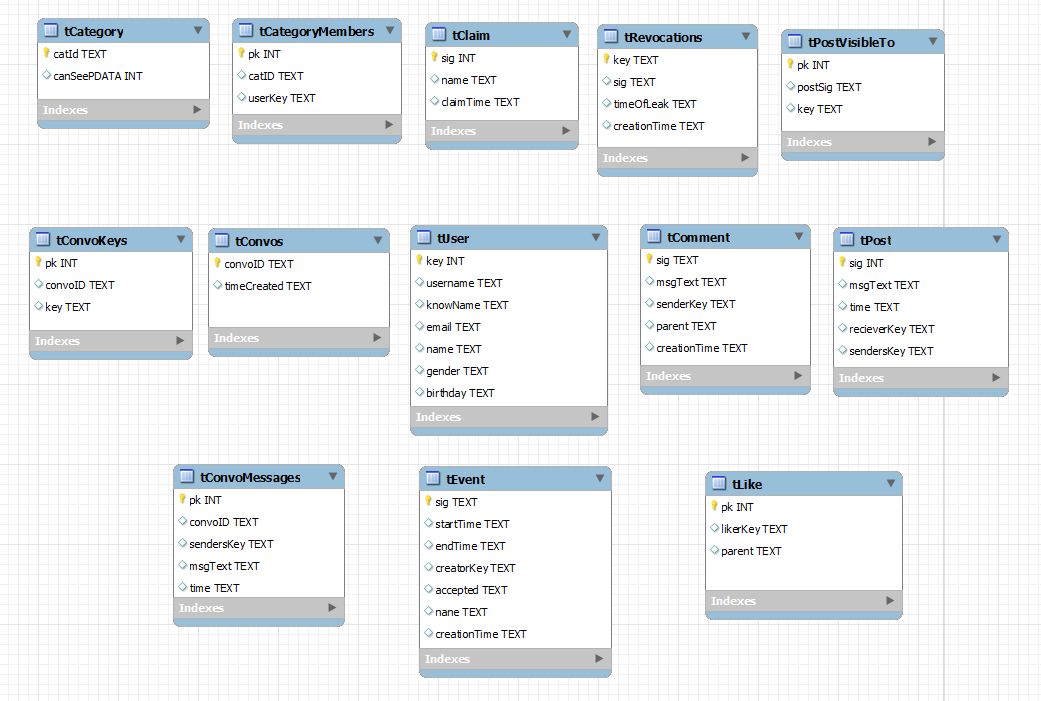
\includegraphics[width=1.4\textwidth]{images/design/db_shot.png}
    \caption{Database Entity Relationship diagram}
    \label{fig:db_er_diag}
\end{figure}
\end{landscape}



\item A number of accessors were added to the Message class for extracing
information from different types of messages.

\item The DBStrings class was added so as to keep SQL query strings seperate
from java code, and to localize them within one namespace. This class merely
contains a large number of static strings.

\item The Logger, Tokenizer,  MessageFactory, and F(ile)IO class were added as
helper classes. Tokenizer was created instead of using javas existing Tokenizer
class because we needed a tokenizer automatically convertable to javascript. A
factory class was required because the Message class cannot contain constructors
not automatically convertable to javascript.

\item The following data bearing classes were created to return structured data
to the HTML/JS frontend. They allow the more powerful java backend to extract
(and format) data from the database before returning a simple class containing
it.
\begin{enumerate}
\item Friend
\item CommentDetails
\item Conversation
\item PostDetails
\end{enumerate}

\item The Turtlenet, TurtlenetImpl, and TurtlenetAsync classes exist to provide
an asynchronous interface between the HTML/JS frontend and the Java backend.
\end{enumerate}



\chapter{Source Code}
We chose to store our source code in a Git repository hosted by Github at: 
\url{https://github.com/thomal/COMP208/}. \par

The repository records all changes to files which allows group members know 
who has modified files, what has been added and what has been deleted. \par

If more than one person edits the same file it is possible to merge together 
the work of each person, often automatically. When more than one person edits 
the same line manual intervention is required to see who's edit should be 
kept. \par

We can also look back at previous revisions of files to figure out where bugs 
were introduced or to resurrect old code that has since been removed but may 
still be useful.


\chapter{Hosting}
We chose Amazon Web Services(AWS) to host the remote server component of Turtlenet and the project website.
The primary reason for this is that AWS offers a free package for the first 12 months of membership. The price after
this is also fairly competitive although we would probably consider other providers if the offer didn't exist. \par

Another advantage of AWS is, due to their size, Amazon have many servers available which lends itself to high 
performance and increased redundancy. Performance isn't a major issue as the Turtlenet remote server acts as little 
more than a middleman. Still, the lower the latency the better. \par

It is uncertain if Amazon has provided any of it's customers personal data to the NSA or any other government sponsored 
agency. This isn't of concern though as very little data is stored by the Turtlenet remote server. Due to the 
distributed nature of Turtlenet all sensitive information is stored in a local database on the users device.


\chapter{Testing}
We chose Amazon Web Services(AWS) to host the remote server component of Turtlenet and the project website.
The primary reason for this is that AWS offers a free package for the first 12 months of membership. The price after
this is also fairly competitive although we would probably consider other providers if the offer didn't exist. \par

Another advantage of AWS is, due to their size, Amazon have many servers available which lends itself to high 
performance and increased redundancy. Performance isn't a major issue as the Turtlenet remote server acts as little 
more than a middleman. Still, the lower the latency the better. \par

It is uncertain if Amazon has provided any of it's customers personal data to the NSA or any other government sponsored 
agency. This isn't of concern though as very little data is stored by the Turtlenet remote server. Due to the 
distributed nature of Turtlenet all sensitive information is stored in a local database on the users device.


\chapter{Turtlenet Website}
The website (www.turtlenet.co.uk), allows users to download the client and view 
details on the project. For example, who has been working on it, and the fine 
print regarding the licensing. These things can not only be useful, but also 
necessary to inform the user what the program is, and why they need it, along 
with providing a suitable means of distribution for the project. Below is a 
short description of the website and its content.


\begin{itemize}
\item Home Page: This is a quick general description about what Turtlenet is, 
providing you with a link to both get the sourcecode for Turtlenet, and the 
client itself.
\item Downloads: Holds the Turtlenet.jar file link, allowing the user to retrieve
the client, as it does other pertinent information regarding any dependencies the
client will need to run.
\item About Us: This page is a small area dedicated to the team behind Turtlenet, 
Ballmer Peak, and our views on the project.
\item Content: This area of the website contains all the contact information for 
our staff, should you need to contact them.
\item FAQs: Frequently Asked Questions about the project come here.
\item License: Finally, here is the legal rambling regarding the license for the 
project.
\end{itemize}

\chapter{Future Development}
\section{Interface Framework}
Currently the interface framework is the Google Web Toolkit (GWT).  This
currently allows the Turtlenet client's interface to run in a web browser of the
user's choosing.  This is because users are already familiar and at home in
their web browsers. This however comes with the downside that different browsers
may have different bugs. With a pure Java GUI, the code is run by a Java
Virtual Machine (JVM) so there is only one platform to worry about whereas
through the use of a browser being a container for the user interface, each with
different layout engines and capabilities, the project can expect to receive bug
reports from at least four different front ends. This is however significantly
mitigated by the fact that GWT compiles different versions of the javascript
source for each large browser, that takes their idiosyncrasies into account.

Given the current difficultly for the avarage user in launching turtlenet, it is
worthwhile to create a small executable that is tailored to each major operating
system and does nothing but start the client and open a web broser to the right
page.

If we were to move to a native GUI then while debugging would be easier, users
wouldn't have a consistant experiance or the comfort of their web browser,
something they already know how to use.

\section{Interface and House Style}
The current interface for the client has been made in such a way that it
provides all of the functionality of the project in fairly easily identifiable
sections.  What it does not do though is look polished enough to be on an
average user's computer yet.  This is most likely due to time constraints
stressing for functionality as opposed to aesthetics, however while not perfect
the current GUI does look far nicer than a native application would and isn't at
all hard on the eyes.

Green has symbolic meaning and was not chosen simply due to the name of the
project - Turtles more often than not have darker colours such as brown or grey
and not green.  Green is often used in healthcare as a sign that something is
either safe or good for you (the green health 'plus' being an example), which is
what Turtlenet aims to be for your communicative efforts.

We feel that the use of the colour green is calming, and the pervasive use of
the colour throughout the GUI leads to a consistant user experiance which builds
a brand identity. A promenant example of this concept is the fact that cadbury
have obtained a UK trademark on Pantone 2685C (purple).

\section{Languages Used}
The project used Java for the back end of the system, SQLite for the Database
and Java converted to JavaScript for the front end.  Java was chosen for the
interoperability of the language - being able to run on whatever has a Java
Virtual Machine (JVM), which are available for most operating systems.  Most
users have the Java Runtime Environment (JRE) installed, which includes JVM so
Java was a good choice for the project.

SQLite is a notably lightweight Database Management System (DBMS) at the expense
of some features that are used in a more complete SQL solution, none of which
were needed for the project.  SQL notably requires you to define data type as
well as the length of the variable as well - sqlite removing this constraint
allowed us to remove field limits without kludgy workarounds.

MongoDB is an attractive alternative, however the relative popularity of SQLite,
combined with the teams prior experiance with it, and greater choice of
libraries contributed to our ultimate decision to use SQLite.

Google Web Toolkit (GWT) allowed one of our developers the capability of writing
code in Java which when compiled creates the required AJAX code which makes RPC
calls to the java backend.  On a technical level we believed this to be quite
elegent, and was one of the reasons we chose GWT for the interface framework.



\begin{appendices}
\appendixpage % Page empty but for page# and "Appendicies" precedes appendicies
\noappendicestocpagenum % Remove the page# from the TOC for that ^ page
\addappheadtotoc % "Appendicies" precedes the listing of appendicies in the TOC

\chapter{Minutes}
\section{Meeting \#1 Minutes (Thursday, 30/01/2014)}
Peter, Luke, Aishah, Leon, Mike
\begin{itemize}
\item Introductions
\item Overview of the project
\item Assigned roles to members
\end{itemize}

\section{Meeting \#2 Minutes (Friday, 31/01/2014)}
Peter, Luke, Aishah, Leon, Mike
\begin{itemize}
\item We ate nice chinese in celebration of the new year
\item If I'm honest this wasnt really a team meeting, more a hunger thing
\end{itemize}

\section{Meeting \#3 Minutes (Tuesday, 04/02/2014)}
Peter, Luke, Aishah, Leon, Mike
\begin{itemize}
\item State out the problems, criticisms on Facebook regarding user privacy issues
    (Leon)
\item Data flow of the system (Luke)
\item User requirements (Luke has done the draft. Refinement to be done by Aishah
    and Peter)
\item Class diagram (to be completed after dataflow diagram and user requirements)
\item Sketches of GUI (Peter and Mike to do this together)
\item GANTT chart and risk assessment (after user requirements has been drafted out)
\item Data dictionary (Aishah)
\item Read about how to implement SQLite (Aishah)
\end{itemize}

\section{Meeting \#4 Minutes (Friday, 07/02/2014)}
Peter, Luke, Aishah, Leon, Louis
\begin{itemize}
\item Introduced Louis Prince to members/project
\item Assigned Roles to requirement sections
\item Team Review date proposed (Wed 19th, Afternoon)
\item Team name: Ballmer Peak
\end{itemize}

\section{Meeting \#5 Minutes (Wednesday, 12/02/2014)}
Peter, Luke, Aishah, Leon, Mike
\begin{itemize}
\item Allocated left over parts
\item Feedback on project and requirements so far
\item Project name: Turtlenet
\item Louis Prince absent from scheduled meeting.
\end{itemize}

\section{Meeting \#6 Minutes (Wednesday, 19/02/2014)}
Peter, Luke, Aishah, Leon, Mike, Louis
\begin{itemize}
\item Discussed design phase, outlined what needs to be done
\item Also outlined who needs to do it, tasklist:
\item Mike - Use Case Diagram, Data Dictionary
\item Leon - Mobile GUI, Sequence Diagram
\item Louis - Web GUI Design, Java/SQLite/HTML-CSS Documentation
\item Aishah - Database Design Doc
\item Peter - Swing/AWT GUI Design, Server GUI Design
\item Luke - Class Interfaces, Protocol, Architecture, Data Flow Diagrams, More Protocol, Psuedocode
\end{itemize}

\section{Meeting \#7 Minutes (Friday, 07/03/2014)}
Peter, Luke, Aishah, Leon, Mike, Louis
\begin{itemize}
\item Business Rules (Peter)
\item Gantt Chart (Mike)
\item Various DB tweaks (Aishah)
\item Merge work into PDF (Luke)
\item Rename GUI design as storyboard
\end{itemize}

\section{Meeting \#8 Minutes (Wednesday, 19/03/2014)}
Peter, Luke, Aishah, Leon, Louis
\begin{itemize}
\item Server.java		(Luke)
\item Client.java		(Luke)
\item Crypto.java		(Luke)
\item NetworkConnection.java	(Luke)
\item Parser.java		(Luke)
\item HTTPServer.java		(Luke)
\item helper classes		(Luke)
\item browser plugins		(Luke)
\item QR Code parser		(Luke)
\item Test harness		(Luke)
\item Installer		(Peter)
\item Website			(Peter [mimic gnome.org])
\item Manual			(Peter)
\item Hardware Server		(Peter)
\item ServerGUI.java		(Leon)
\item First run config	(Leon)
\item Database.java		(Mike, Aishah)
\item SQLite Database		(Aishah)
    \begin{itemize}
    \item Database connection
    \item Create DB
    \end{itemize}
\item Logo and Graphic Design	(Aishah)
\item GWT interface		(Louis)
    \begin{itemize}
    \item Stubs in interface
    \item error on failure to connect
    \item Add public keys
    \item Categorise users
    \item Post to your wall
    \item Read others wall posts
    \item Post to anothers wall
    \item Events create and recieve
    \item Chat
    \item Comment posts and comments
    \item Like posts and comments
    \end{itemize}
\end{itemize}

\section{Meeting \#9 Minutes (Friday, 21/03/2014)}
Peter, Luke, Aishah, Mike, Louis
\begin{itemize}
\item Everyone can build project
\item DB Connection
\item GWT Interface stubs
\item Stubs for other classes
\item Manual contents page
\item Create table statements
\item Compile remote server as a JAR
\item Server GUI, start up and shut down
\end{itemize}
Leon absent.

\section{Meeting \#10 Minutes (Friday, 28/03/2014)}
Peter, Luke, Aishah, Leon, Mike, Louis
\begin{itemize}
\item Fix manual stuff, add makefile, finish initial test setup (luke)
\item Create tables from Database.java (aishah/mike)
\item GWT Interface (louis)
\item Start/Stop server via gui (leon)
\item Webstie Prototype (peter)
\item Document regarding hashing for various classes (luke)
\end{itemize}

\section{Meeting \#11 Minutes (Sunday, 13/04/2014)}
Peter, Luke, Aishah, Louis
\begin{itemize}
\item Progress Recap: (Luke)
    \begin{itemize}
    \item Added testing
    \item Added logger
    \item Implemented createDatabase to execute aishahs create table SQL queries
    \item Message::XgetY methods
    \item Altered frontend to start turtlenet when it starts, and stop it when the tab is closed
    \end{itemize}
\item Re: Enable -strict for compiling frontend (Luke/Louis)
\item Installer (Luke)
\item Store the signature (String) for posts and comments (Aishah/Mike)
\item SQL for database methods (Aishah/Mike)
\item Implement database methods (Aishah/Mike)
\item Start/Stop server via gui (Leon)
\item Website Prototype (Peter)
\item Call appropriate Database.getX methods (Louis)
\end{itemize}
Leon, Mike not present.

\section{Meeting \#12 Minutes (Saturday, 19/04/2014)}
Peter, Luke, Aishah, Leon, Mike, Louis
\begin{itemize}
\item Website finally unveiled
\item Reassignment of some tasks (prioritization)
\item Mostly a formality to remind people of deadlines
\end{itemize}

\section{Meeting \#13 Minutes (Friday 02/05/2014)}
Peter, Luke, Aishah, Leon, Mike, Louis
\begin{itemize}
\item Assigned final weeks tasks and roles for submitting the portfolio
\item Updates Requirements (Aishah)
\item Updates Design (Aishah)
\item Website (Leon)
\item Source Code (Leon)
\item Personal Statements (All)
\item Deviations Requirements (Luke)
\item Deviations Design (Luke)
\item Hashes (Luke)
\item User Manual (Mike)
\item Future Development Continued (Mike)
\item Hosting AWS (Louis)
\item Testing Automated/Blackbox (Louis)
\end{itemize}

\chapter{Screenshots}
\begin{centering}
\begin{figure}[p] 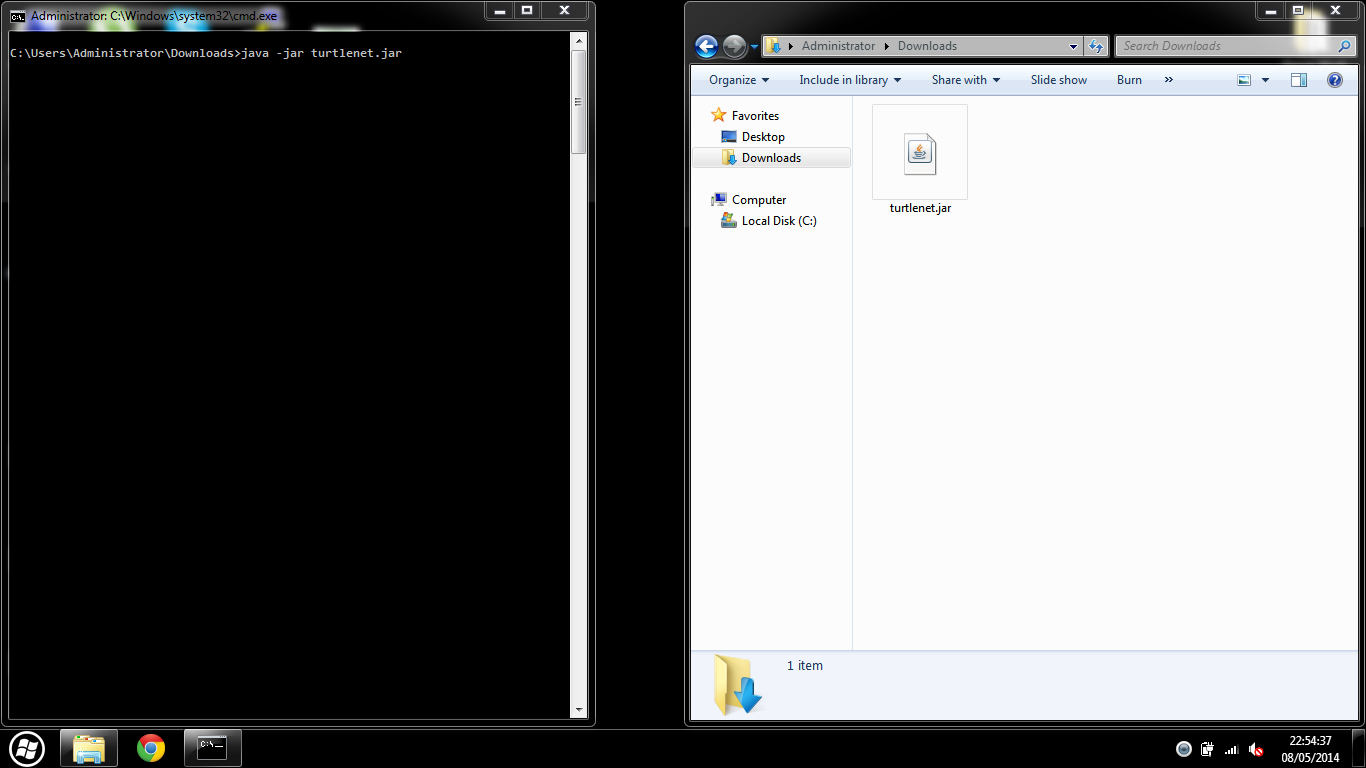
\includegraphics[scale=0.4]{images/screenshots/1startprogram.png} \end{figure}
\begin{figure}[p] 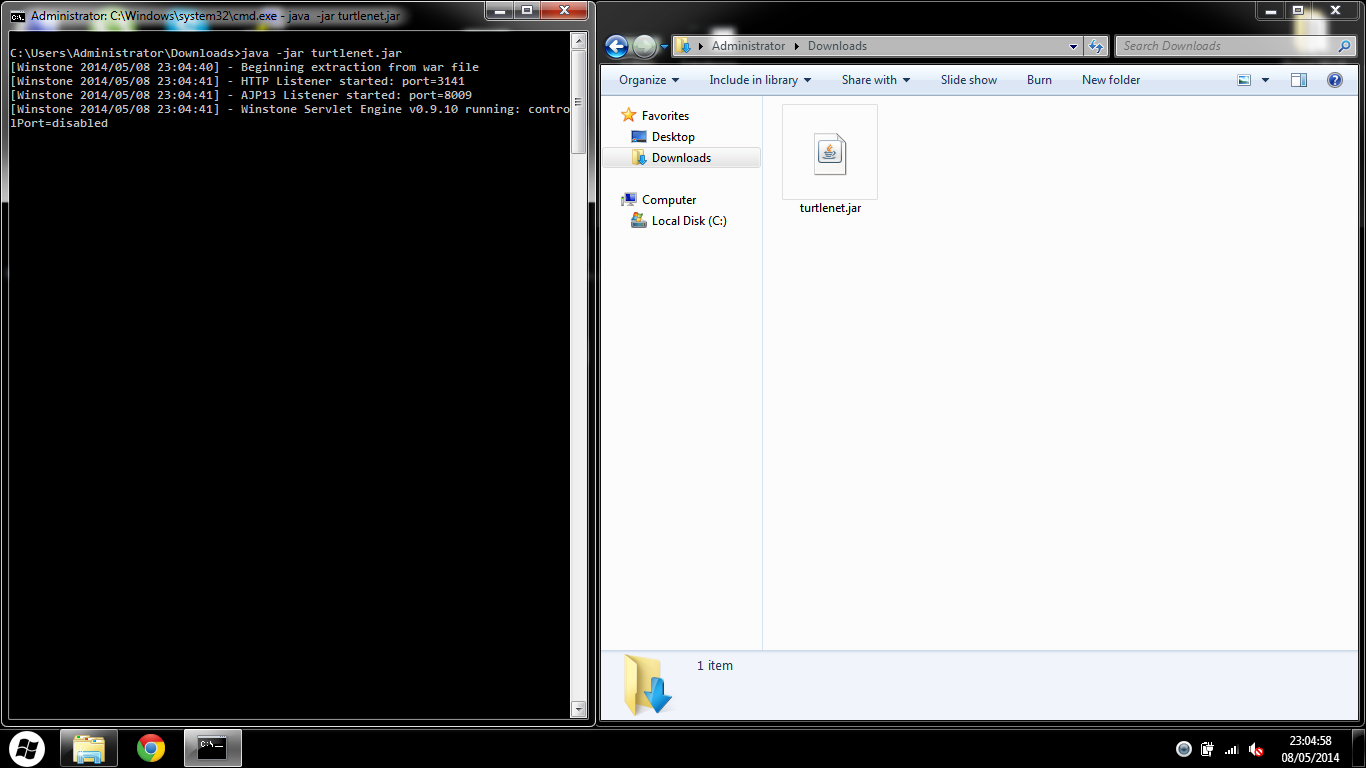
\includegraphics[scale=0.4]{images/screenshots/2running.png} \end{figure}
\begin{figure}[p] 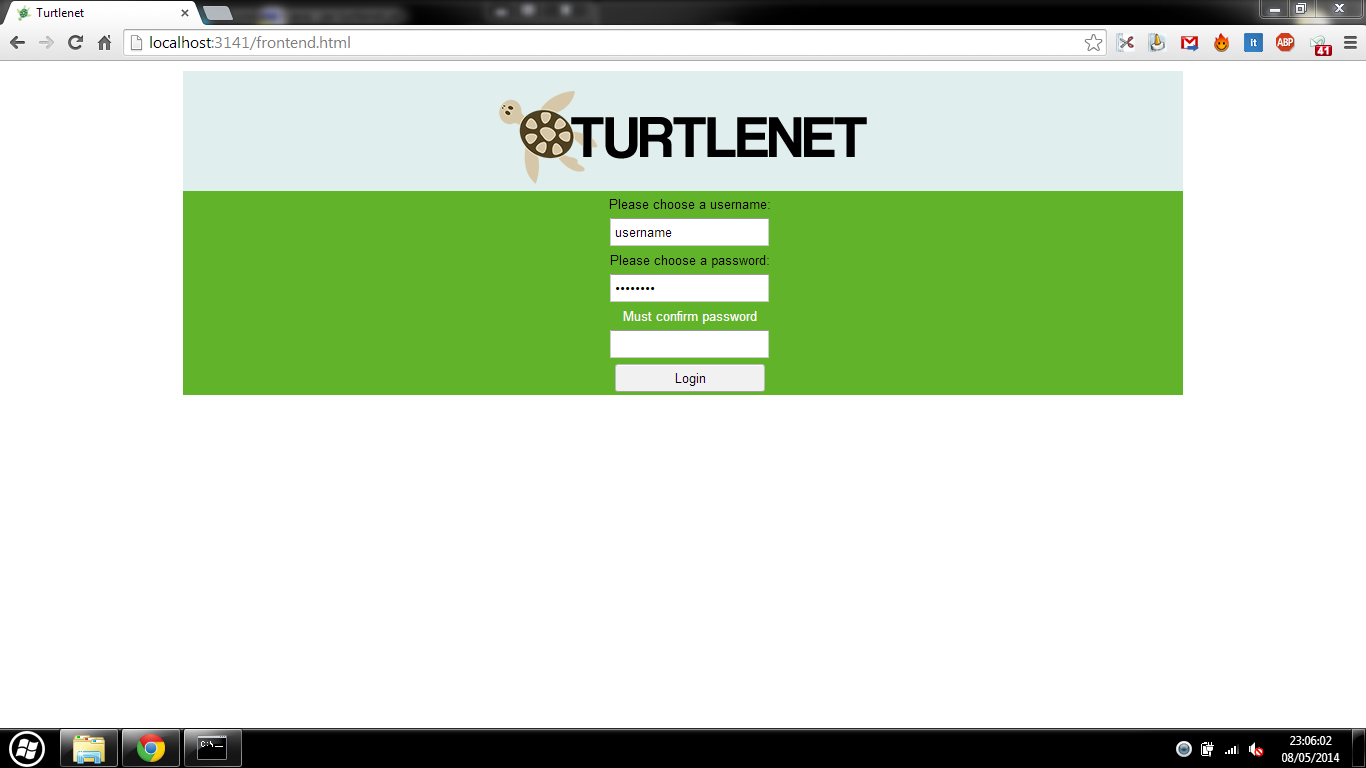
\includegraphics[scale=0.5]{images/screenshots/4login.png} \end{figure}
\begin{figure}[p] 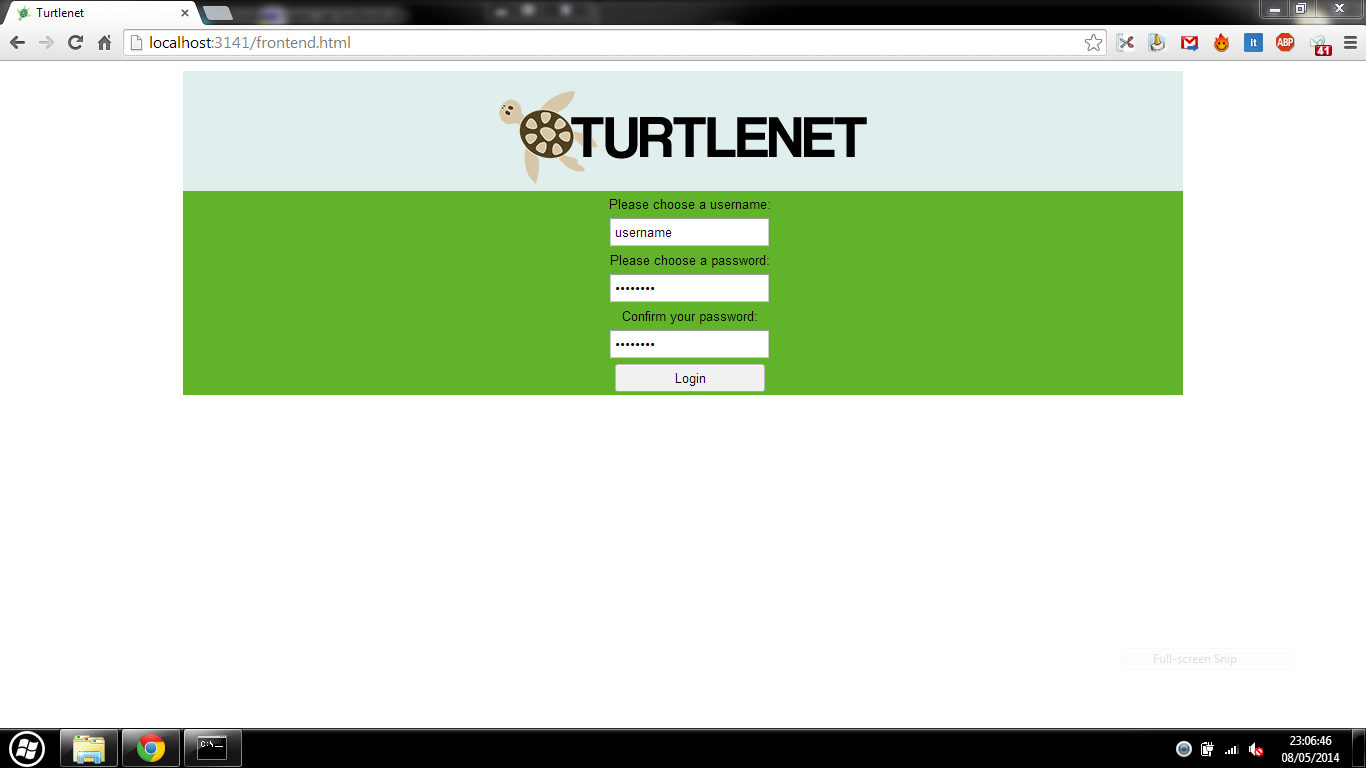
\includegraphics[scale=0.5]{images/screenshots/5loginagain.png} \end{figure}
\begin{figure}[p] 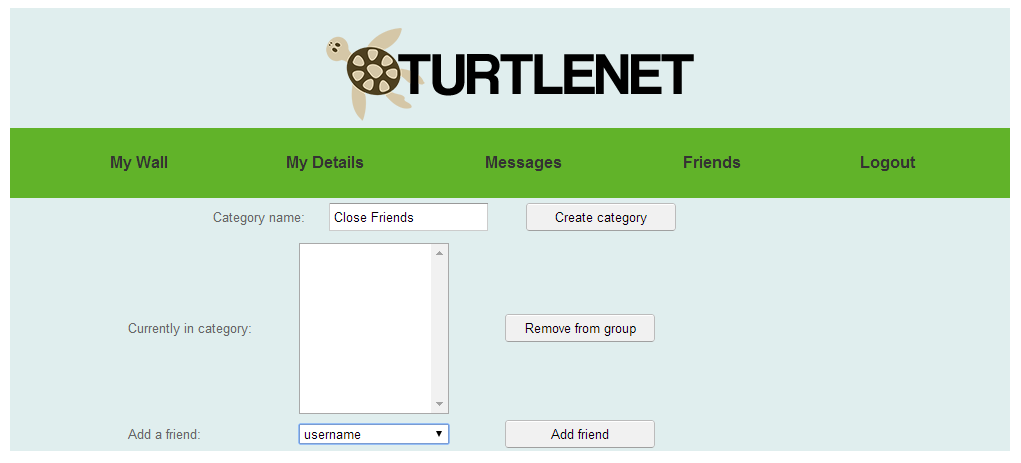
\includegraphics[scale=0.5]{images/screenshots/crop1.png} \end{figure}
\begin{figure}[p] 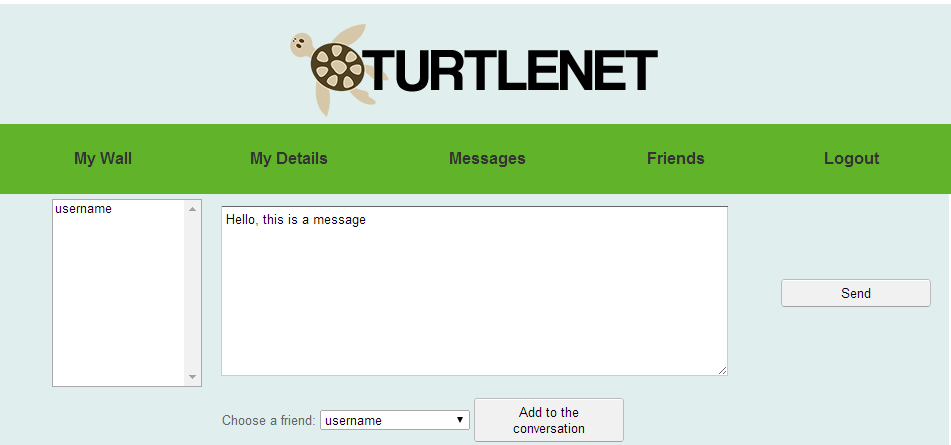
\includegraphics[scale=0.5]{images/screenshots/crop2.png} \end{figure}
\begin{figure}[p] 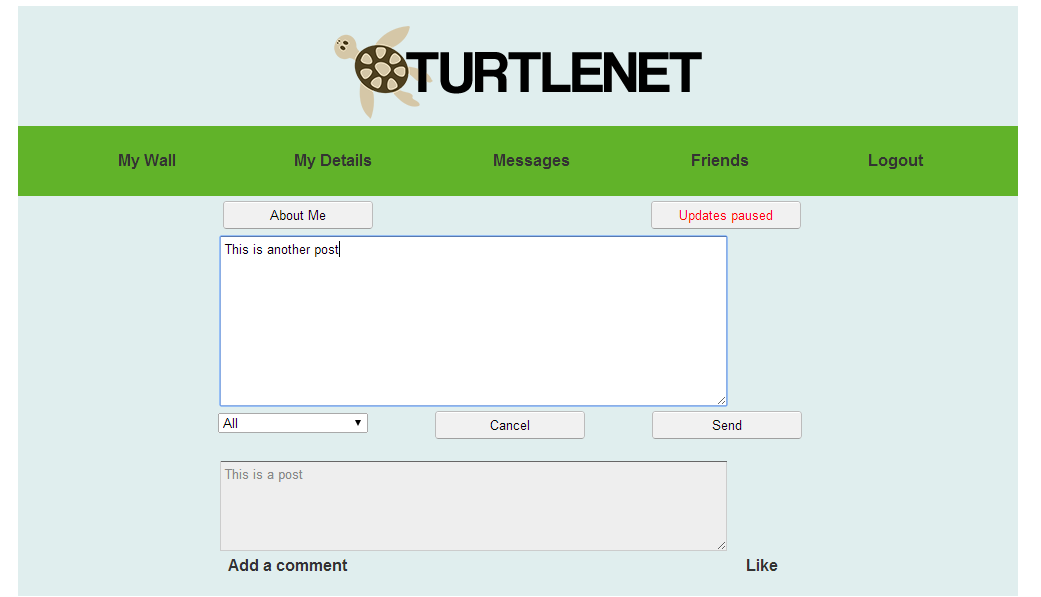
\includegraphics[scale=0.5]{images/screenshots/crop3.png} \end{figure}
\begin{figure}[p] 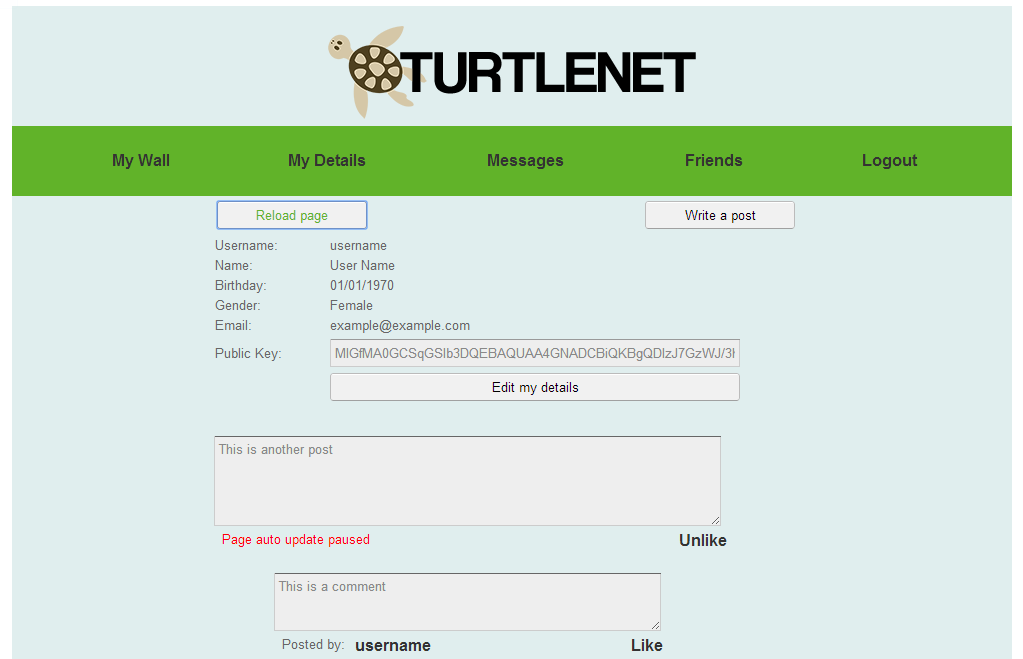
\includegraphics[scale=0.5]{images/screenshots/crop4.png} \end{figure}
\begin{figure}[p] 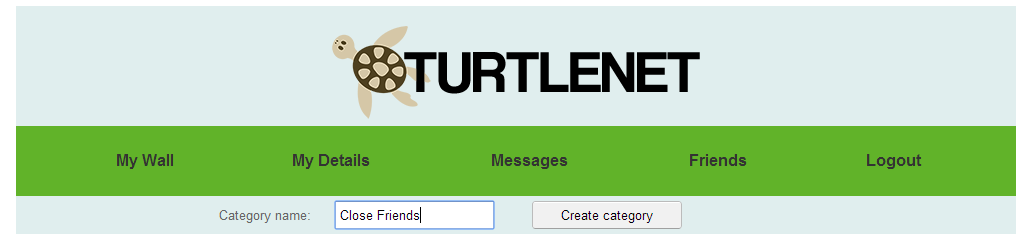
\includegraphics[scale=0.5]{images/screenshots/crop5.png} \end{figure}
\begin{figure}[p] 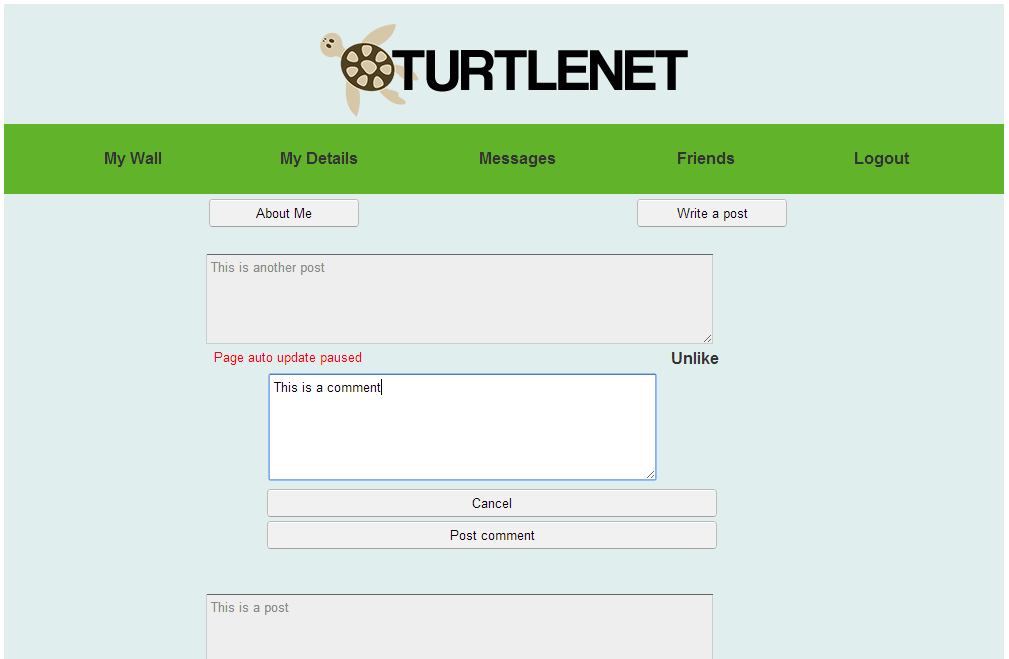
\includegraphics[scale=0.5]{images/screenshots/crop6.png} \end{figure}
\begin{figure}[p] 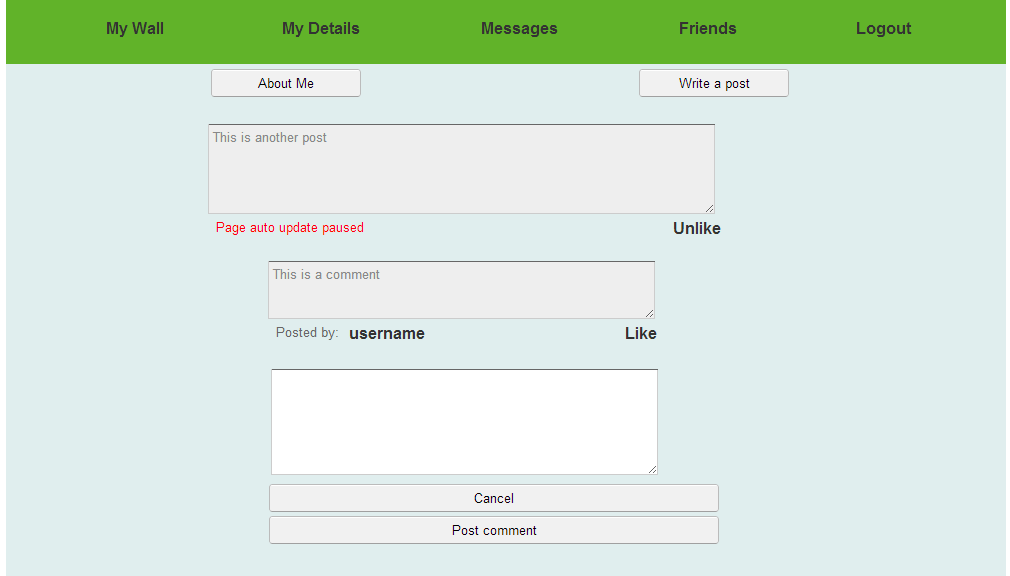
\includegraphics[scale=0.5]{images/screenshots/crop7.png} \end{figure}
\begin{figure}[p] 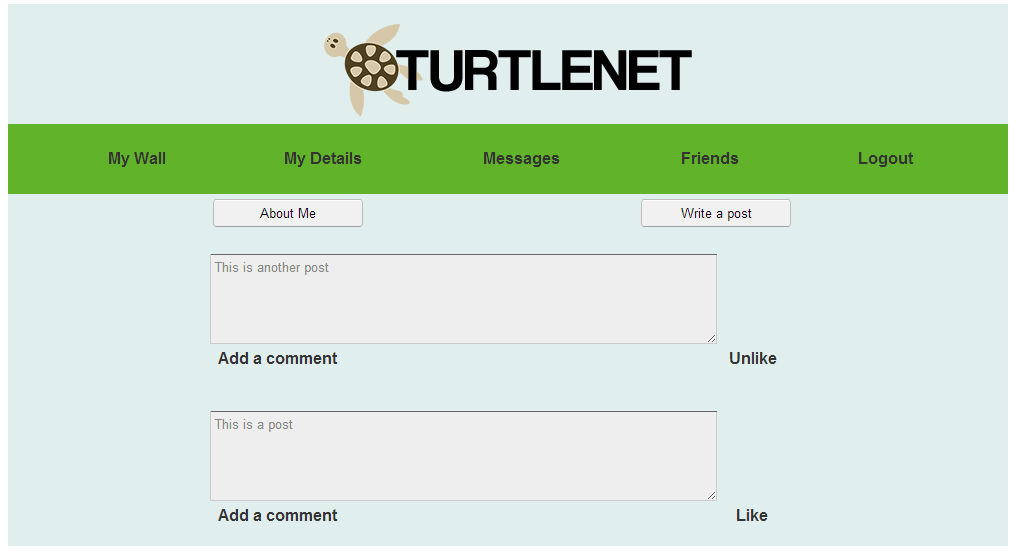
\includegraphics[scale=0.5]{images/screenshots/crop8.png} \end{figure}
\begin{figure}[p] 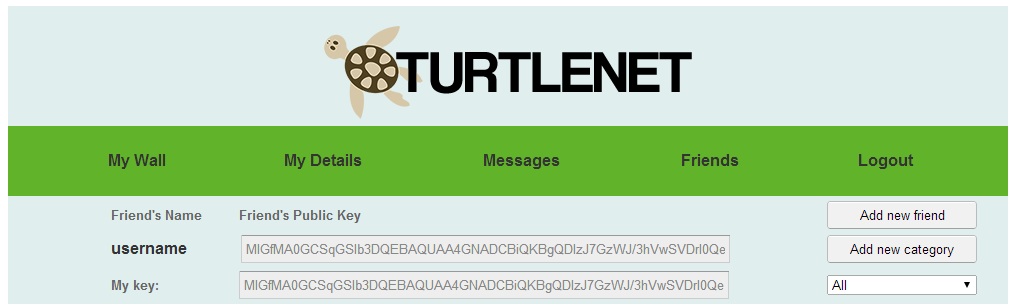
\includegraphics[scale=0.5]{images/screenshots/crop9.png} \end{figure}
\begin{figure}[p] 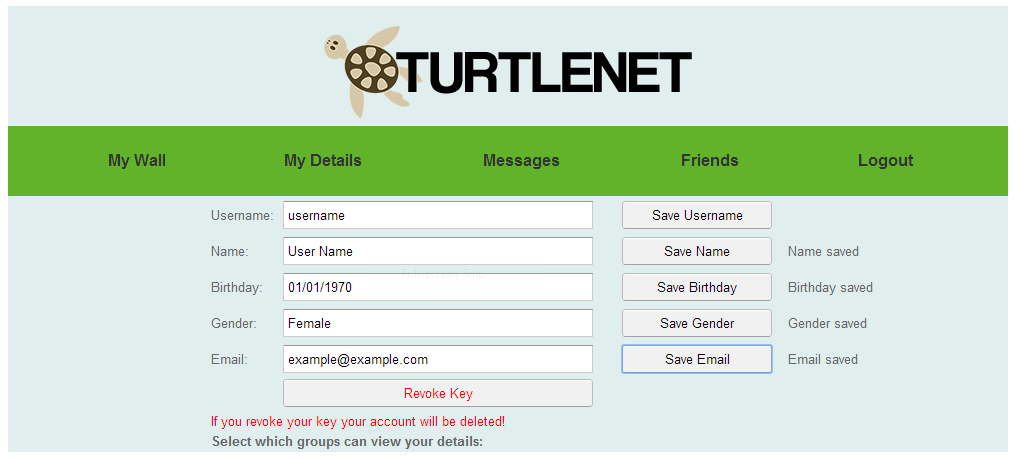
\includegraphics[scale=0.5]{images/screenshots/crop10.png} \end{figure}
\begin{figure}[p] 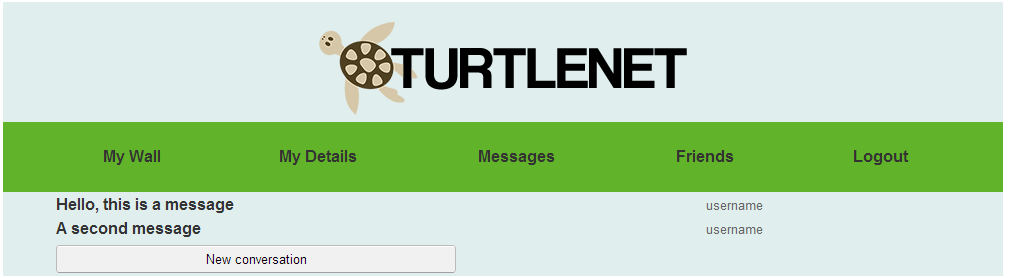
\includegraphics[scale=0.5]{images/screenshots/crop11.png} \end{figure}
\begin{figure}[p] 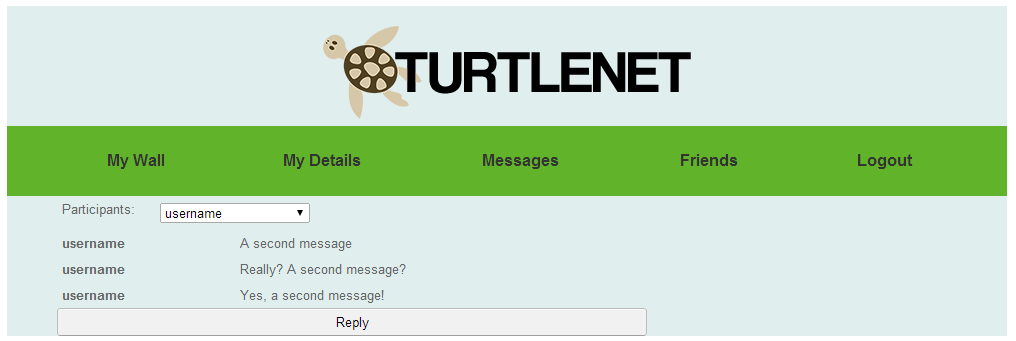
\includegraphics[scale=0.5]{images/screenshots/crop12.png} \end{figure}
\begin{figure}[p] 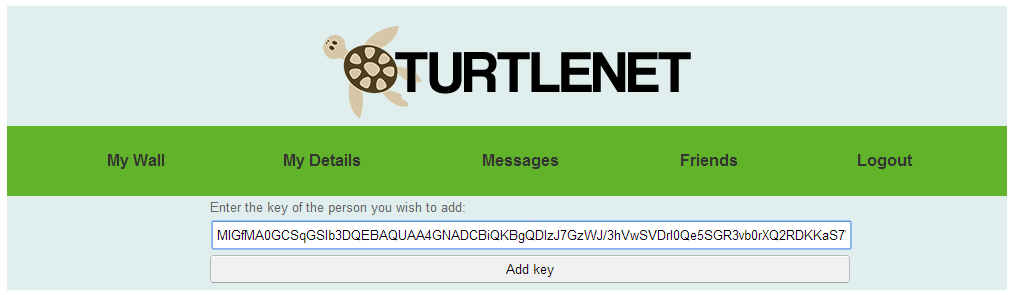
\includegraphics[scale=0.5]{images/screenshots/crop13.png} \end{figure}
\end{centering}

\chapter{Source Listing}
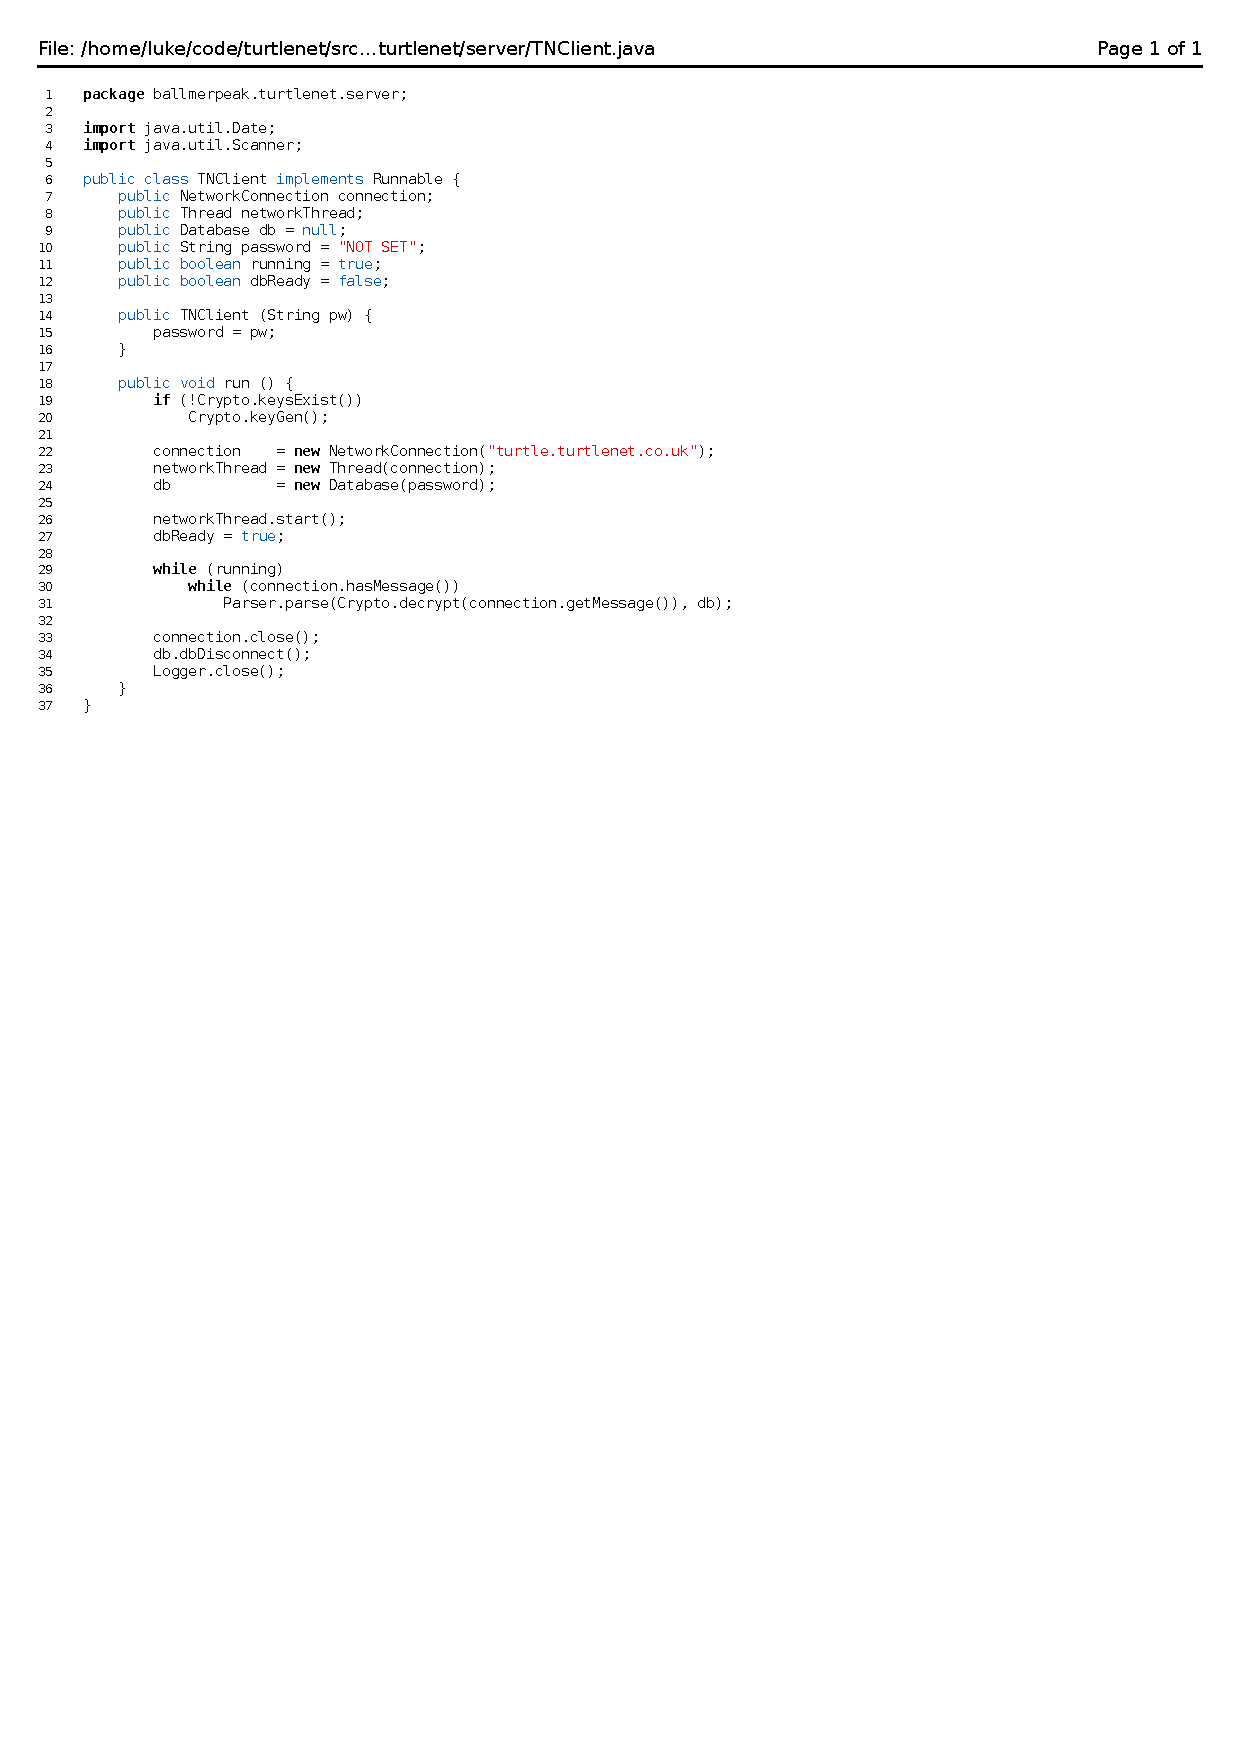
\includepdf[pages={-}]{./text/appendicies/source/7TNClient.pdf}
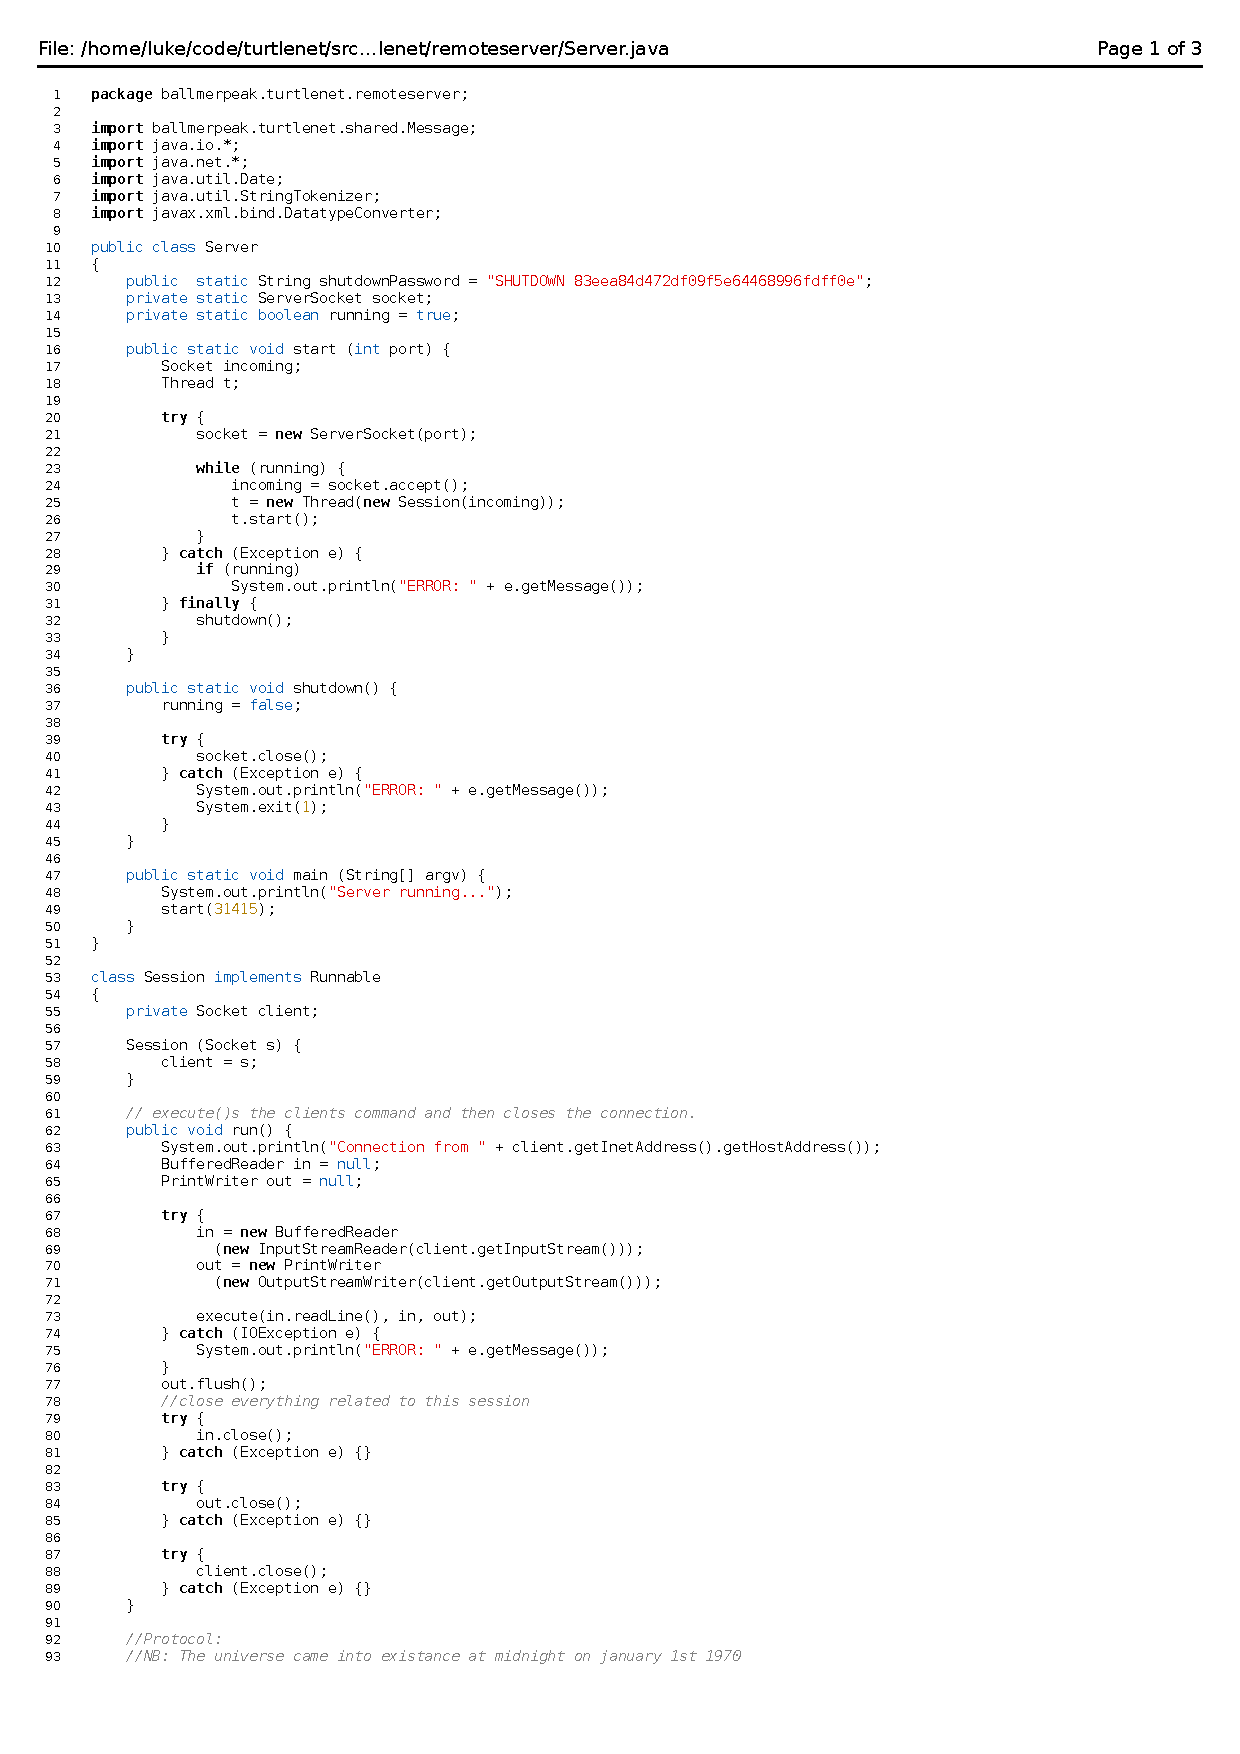
\includepdf[pages={-}]{./text/appendicies/source/0Server.pdf}
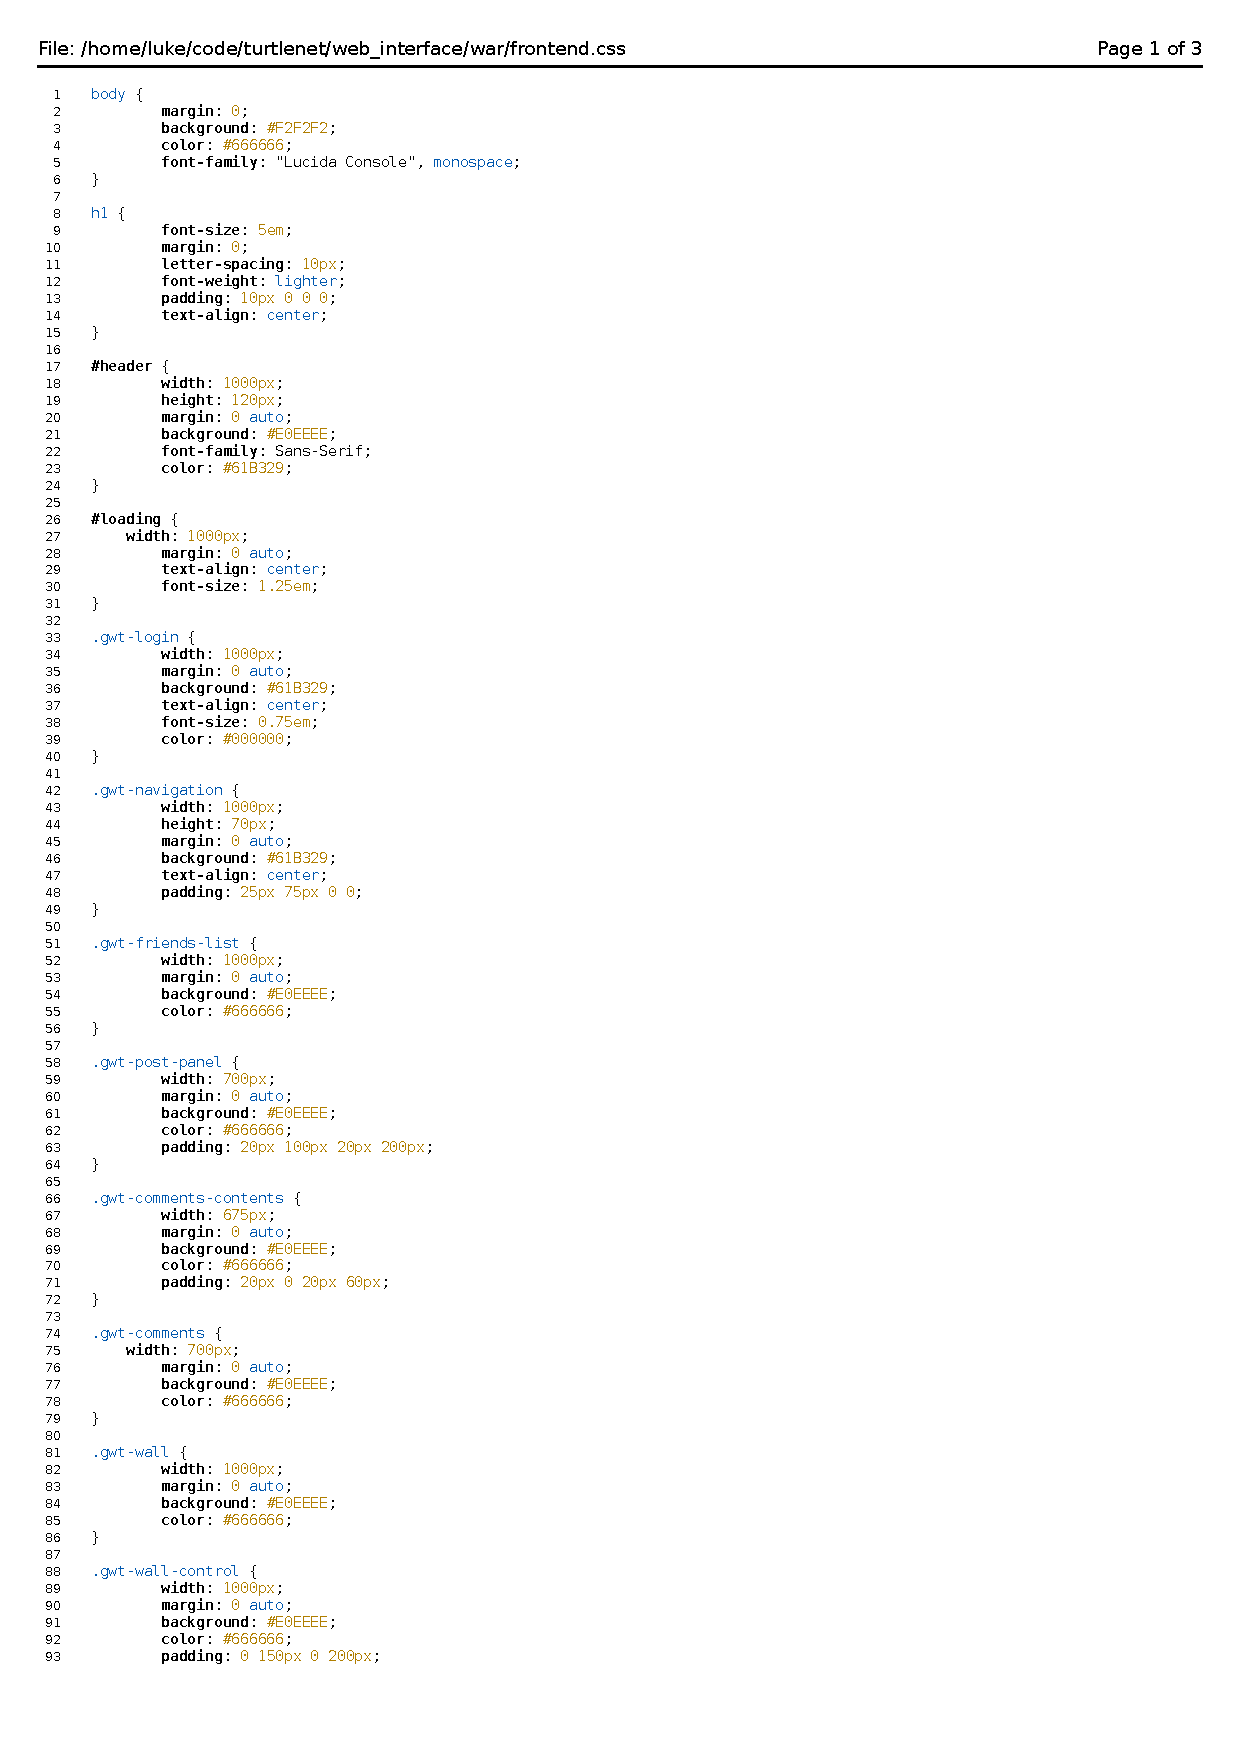
\includepdf[pages={-}]{./text/appendicies/source/1frontend.pdf}
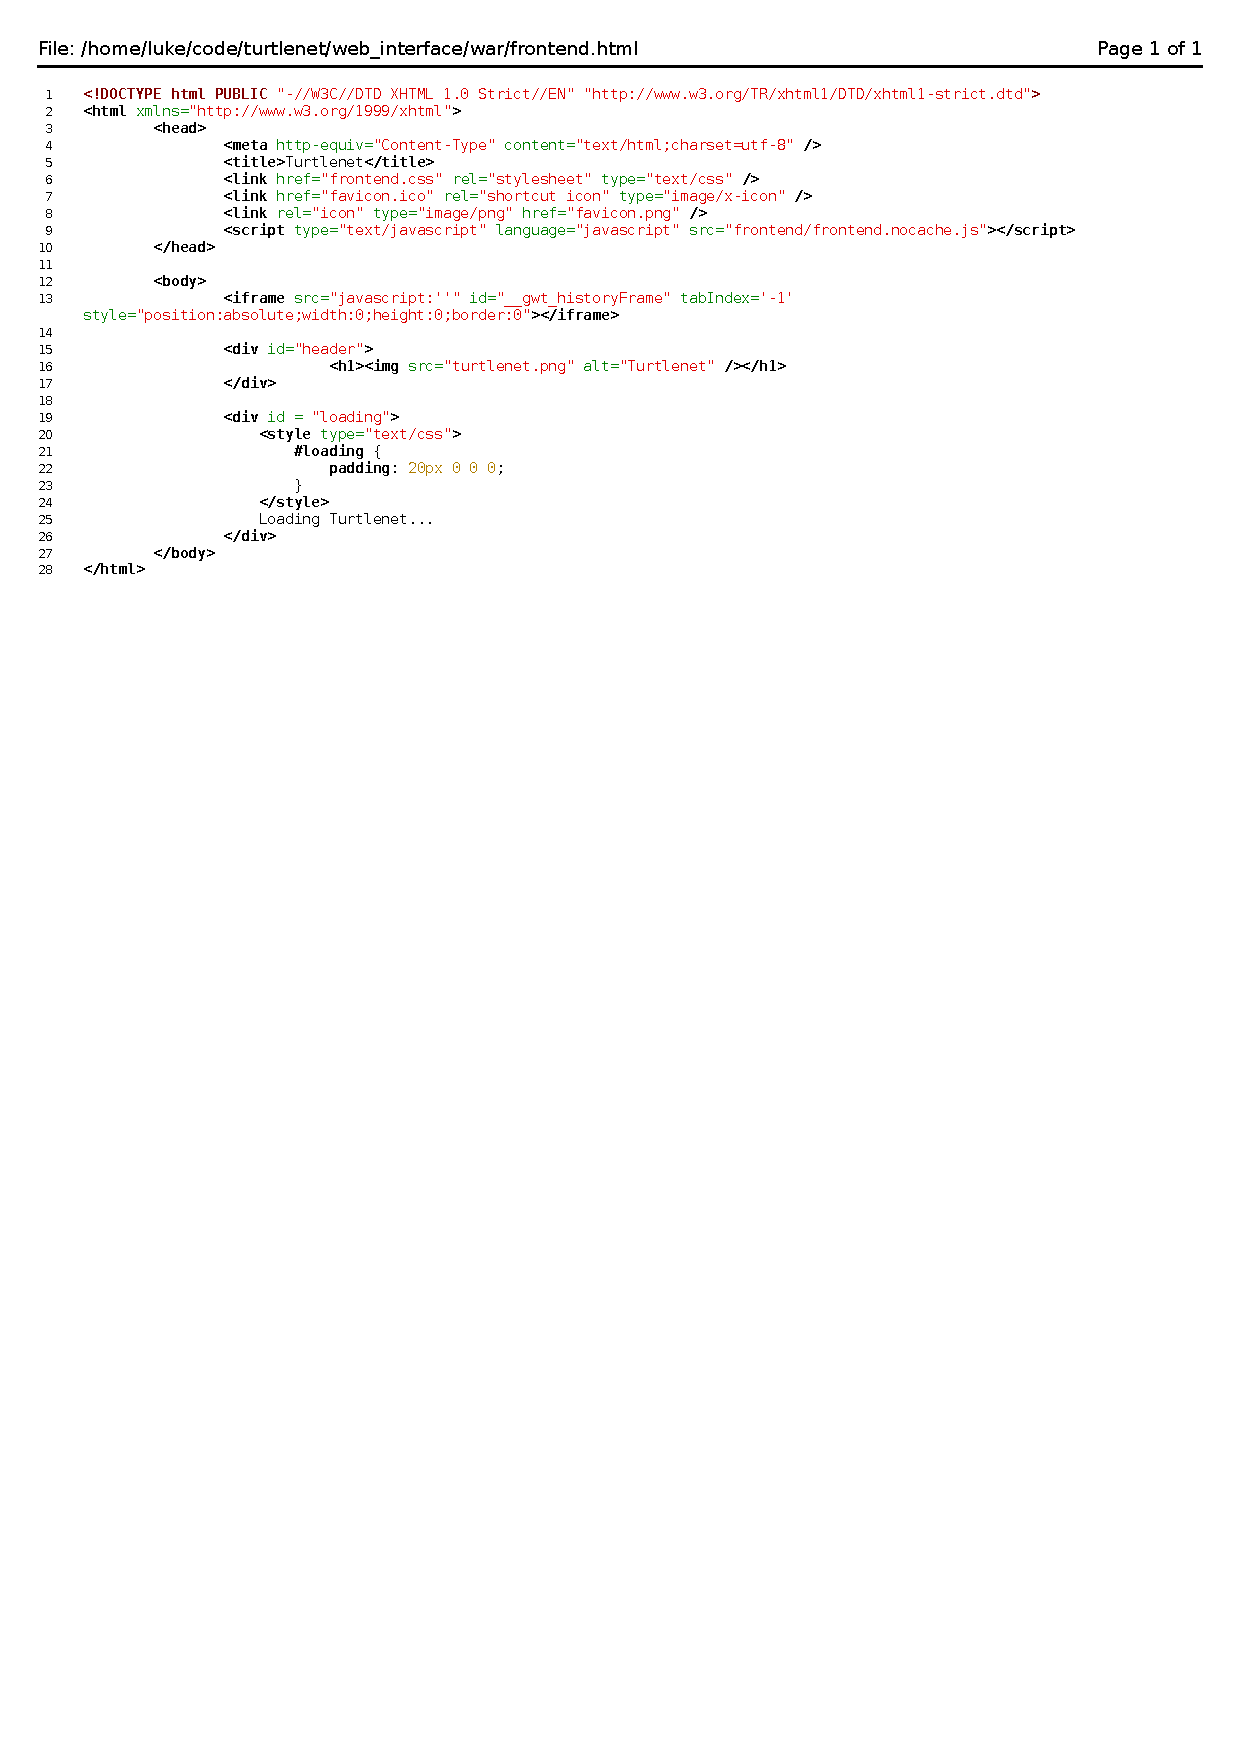
\includepdf[pages={-}]{./text/appendicies/source/2frontend.pdf}
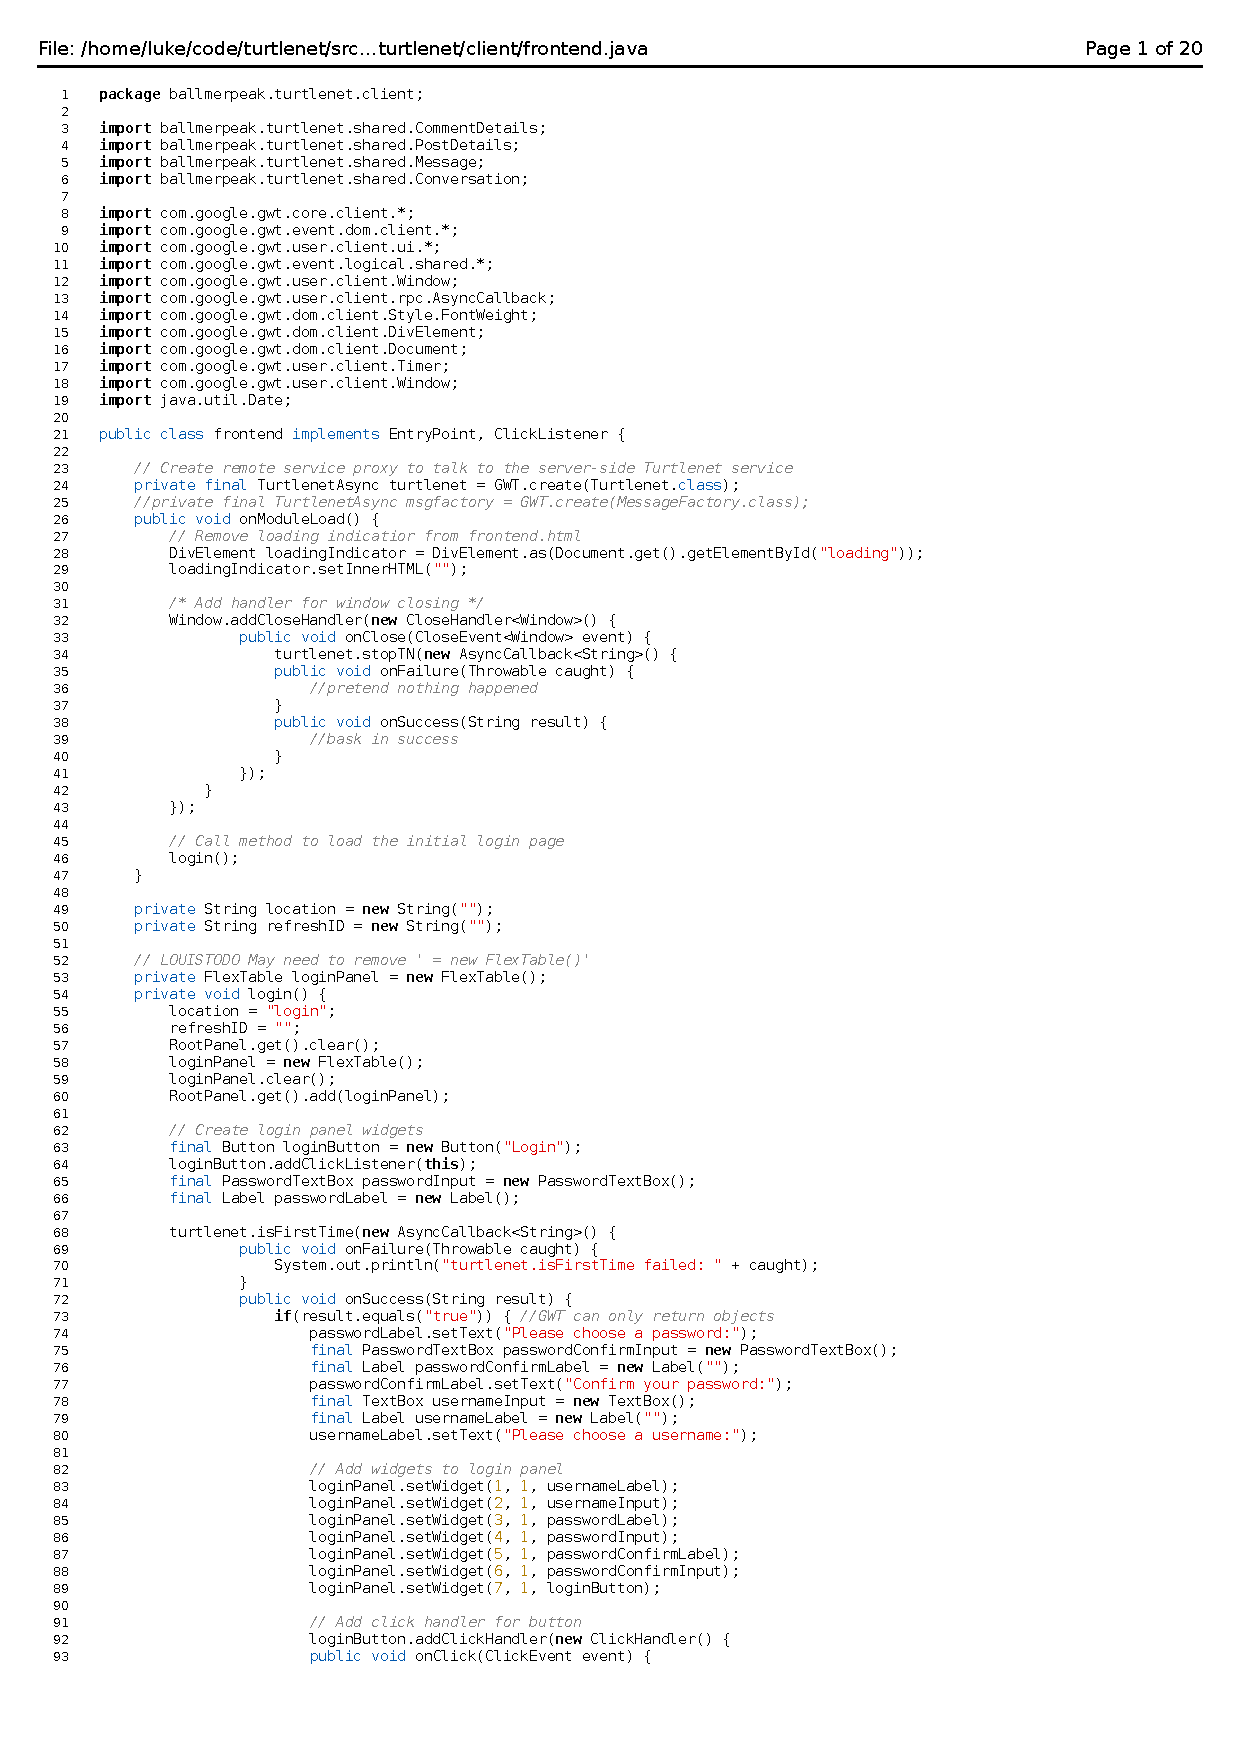
\includepdf[pages={-}]{./text/appendicies/source/3frontend.pdf}
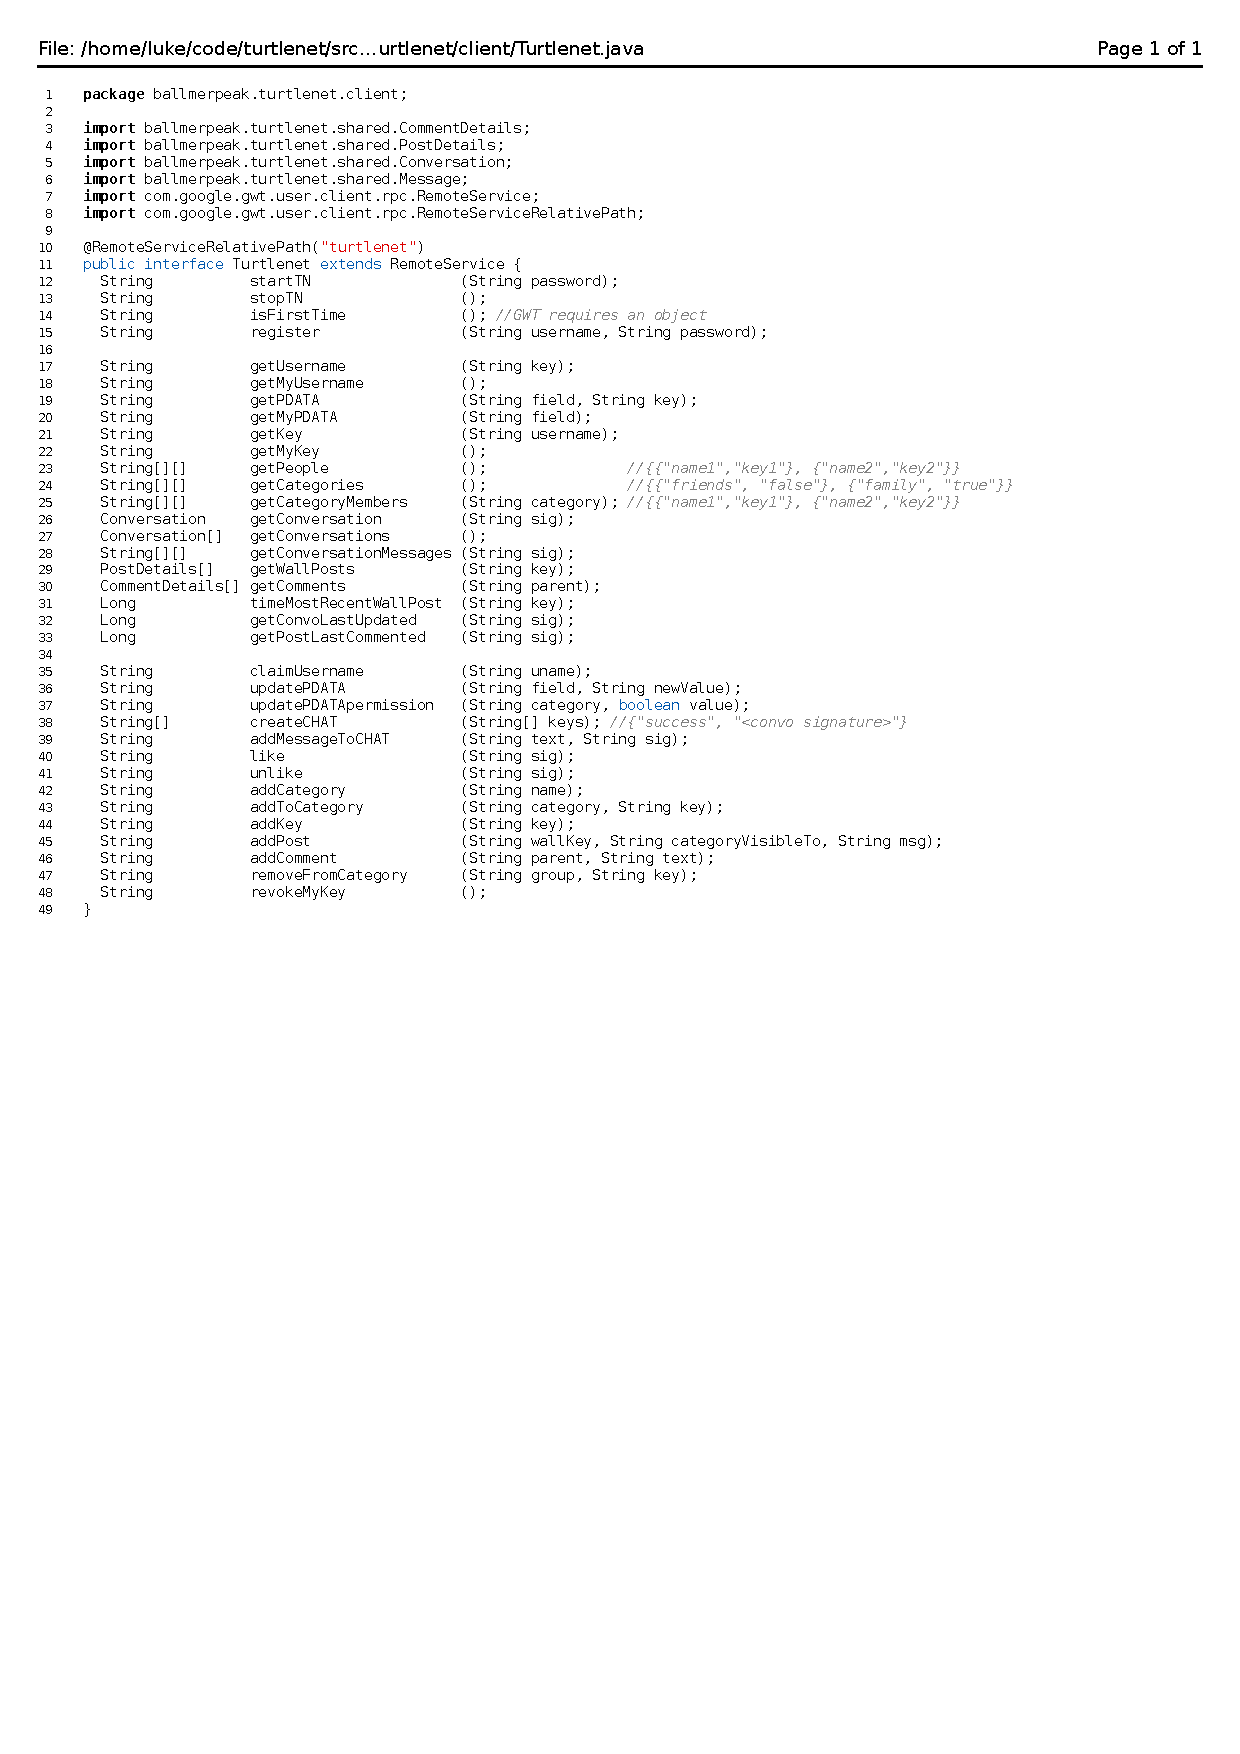
\includepdf[pages={-}]{./text/appendicies/source/4Turtlenet.pdf}
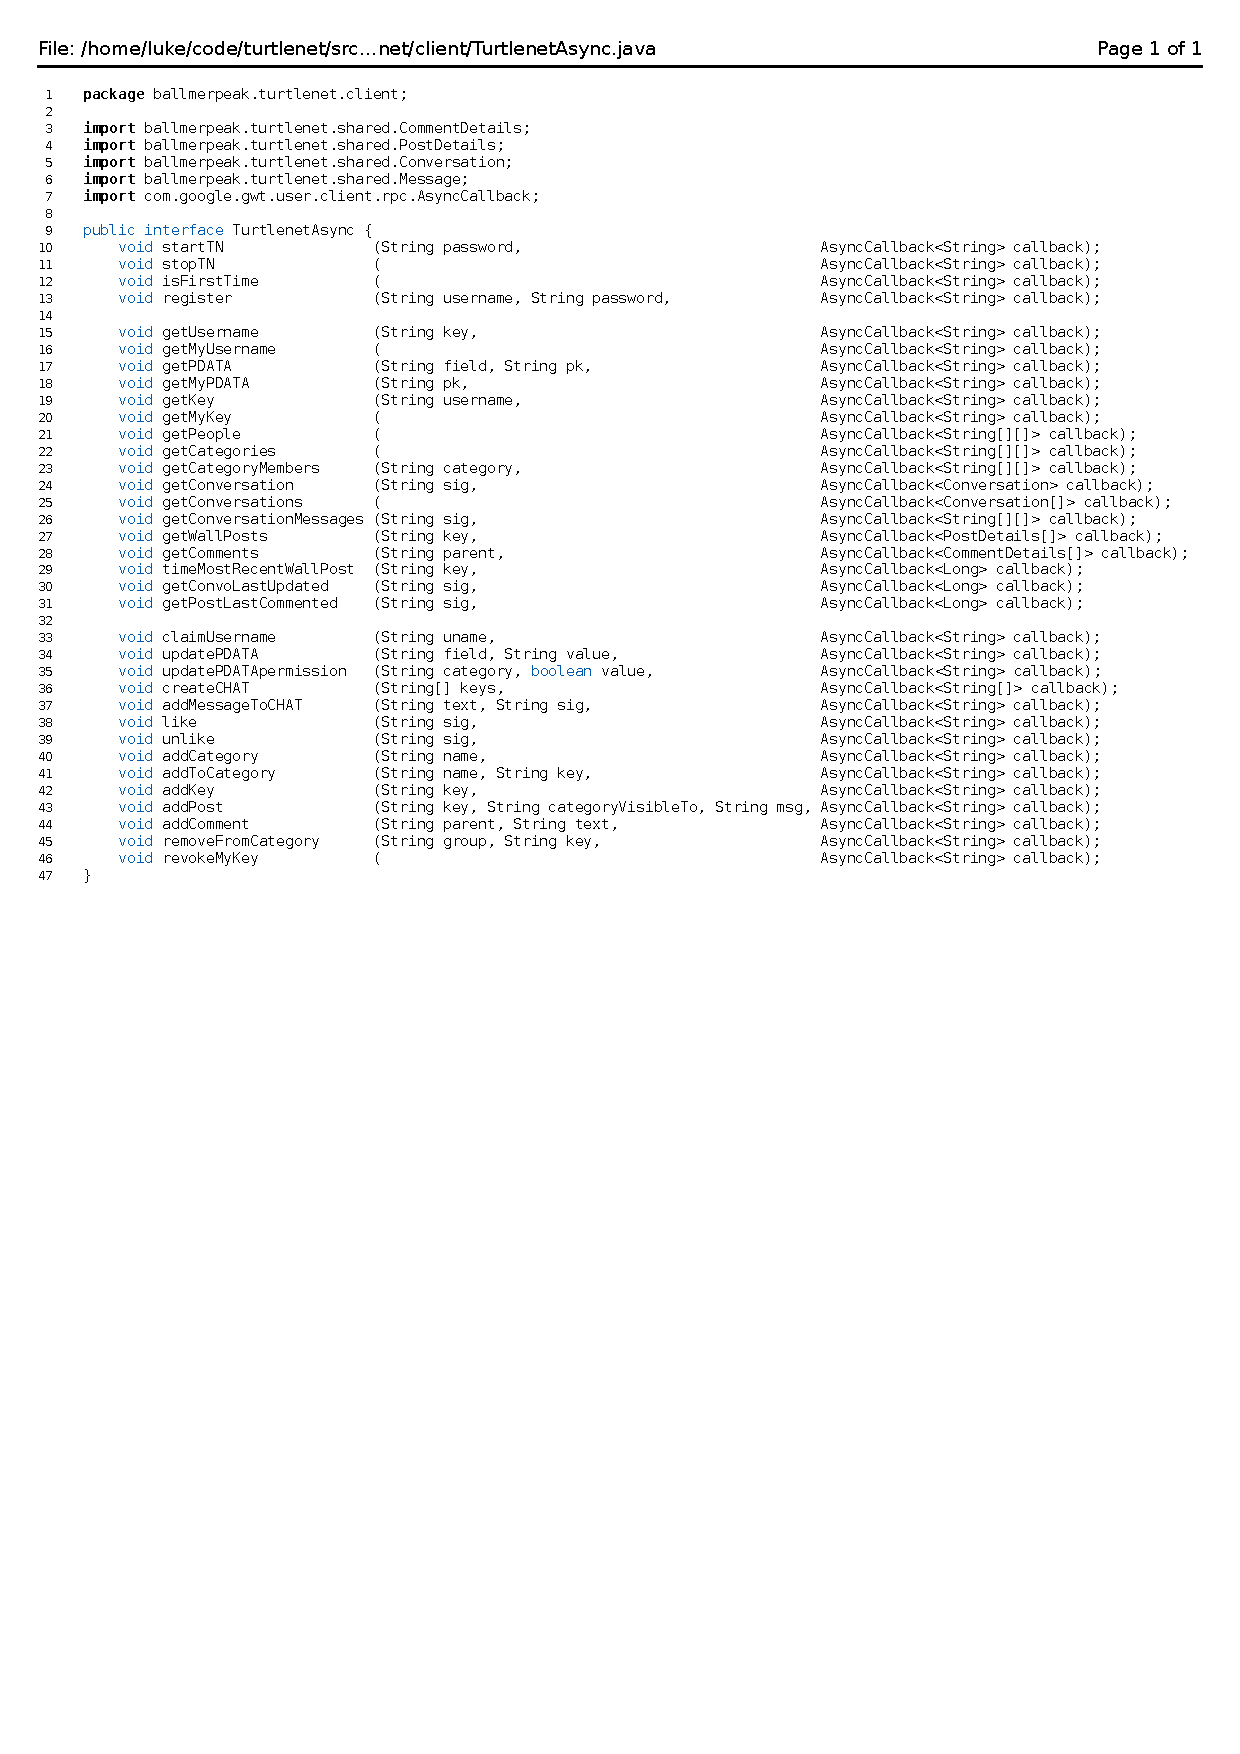
\includepdf[pages={-}]{./text/appendicies/source/5TurtlenetAsync.pdf}
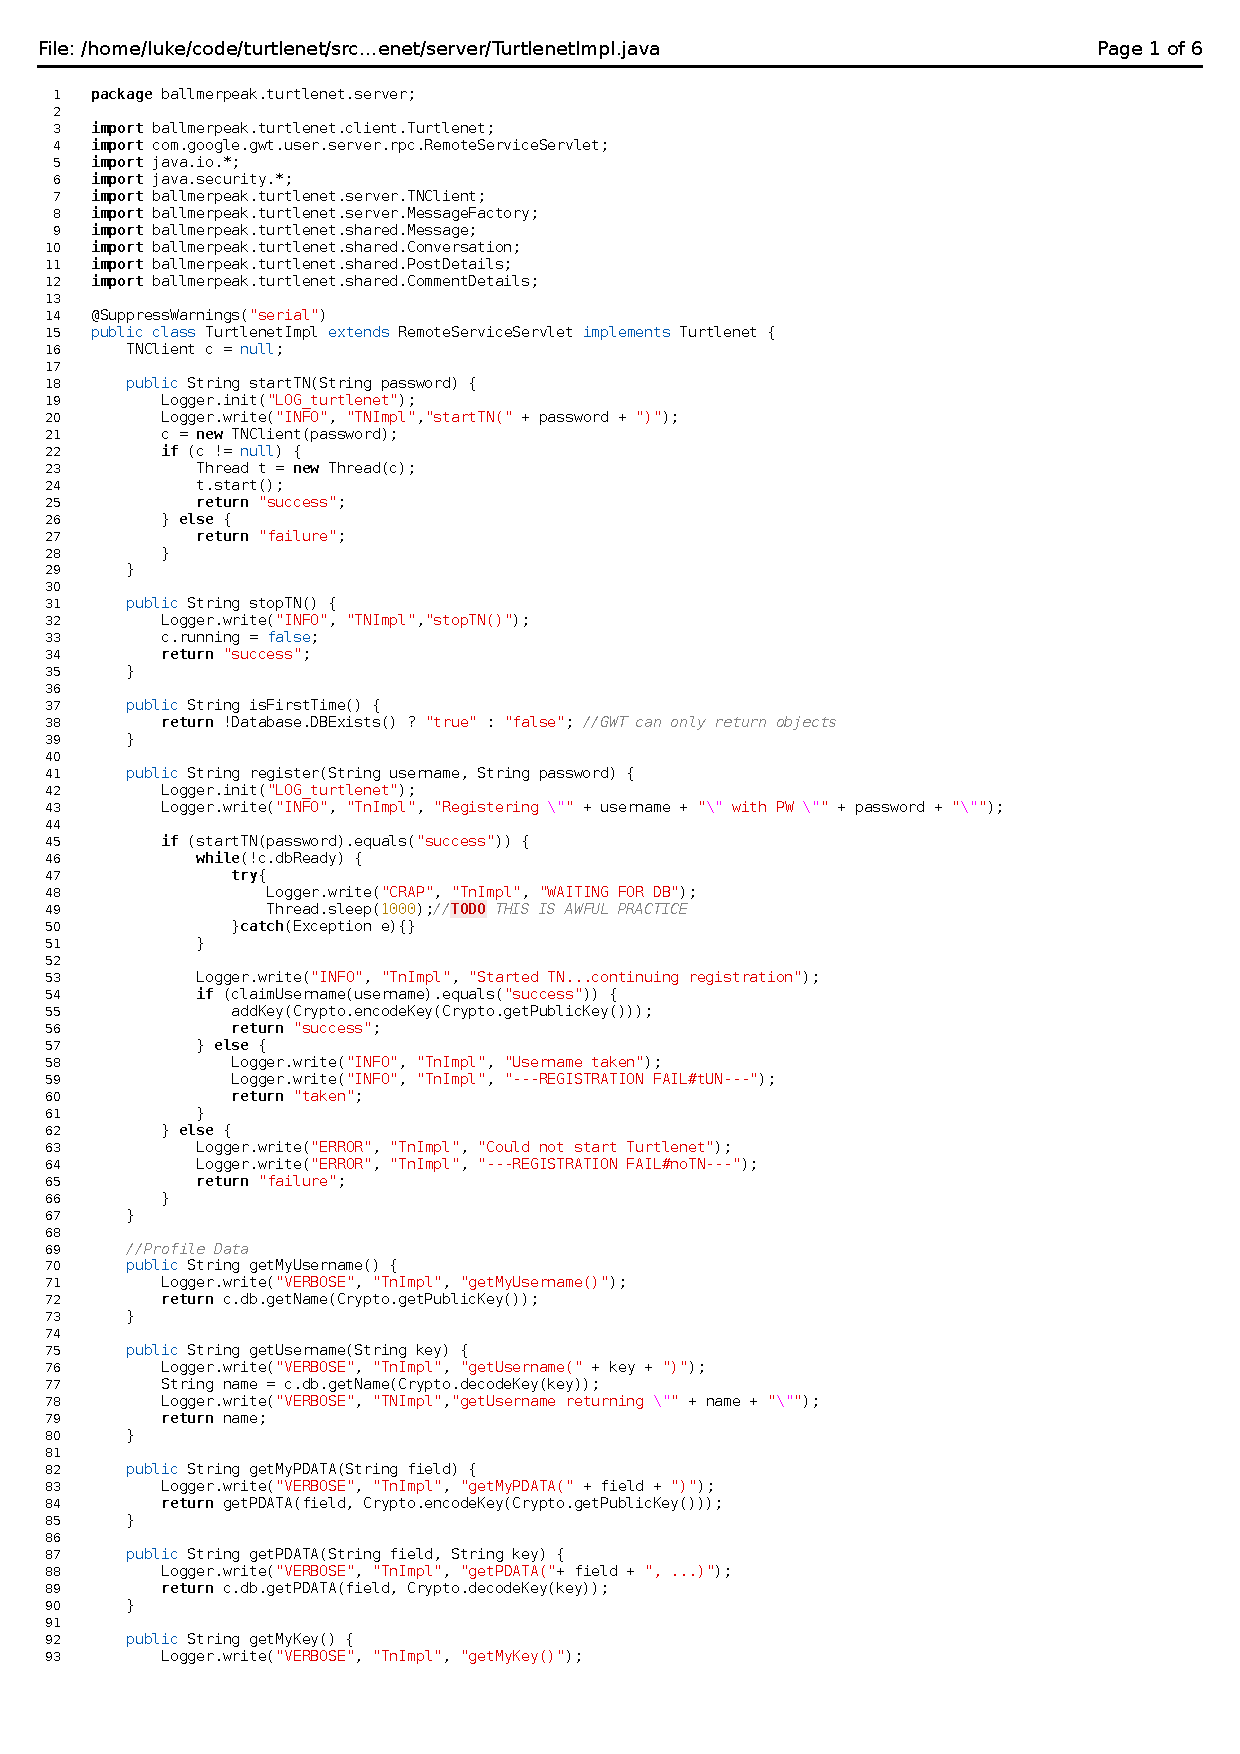
\includepdf[pages={-}]{./text/appendicies/source/6TurtlenetImpl.pdf}
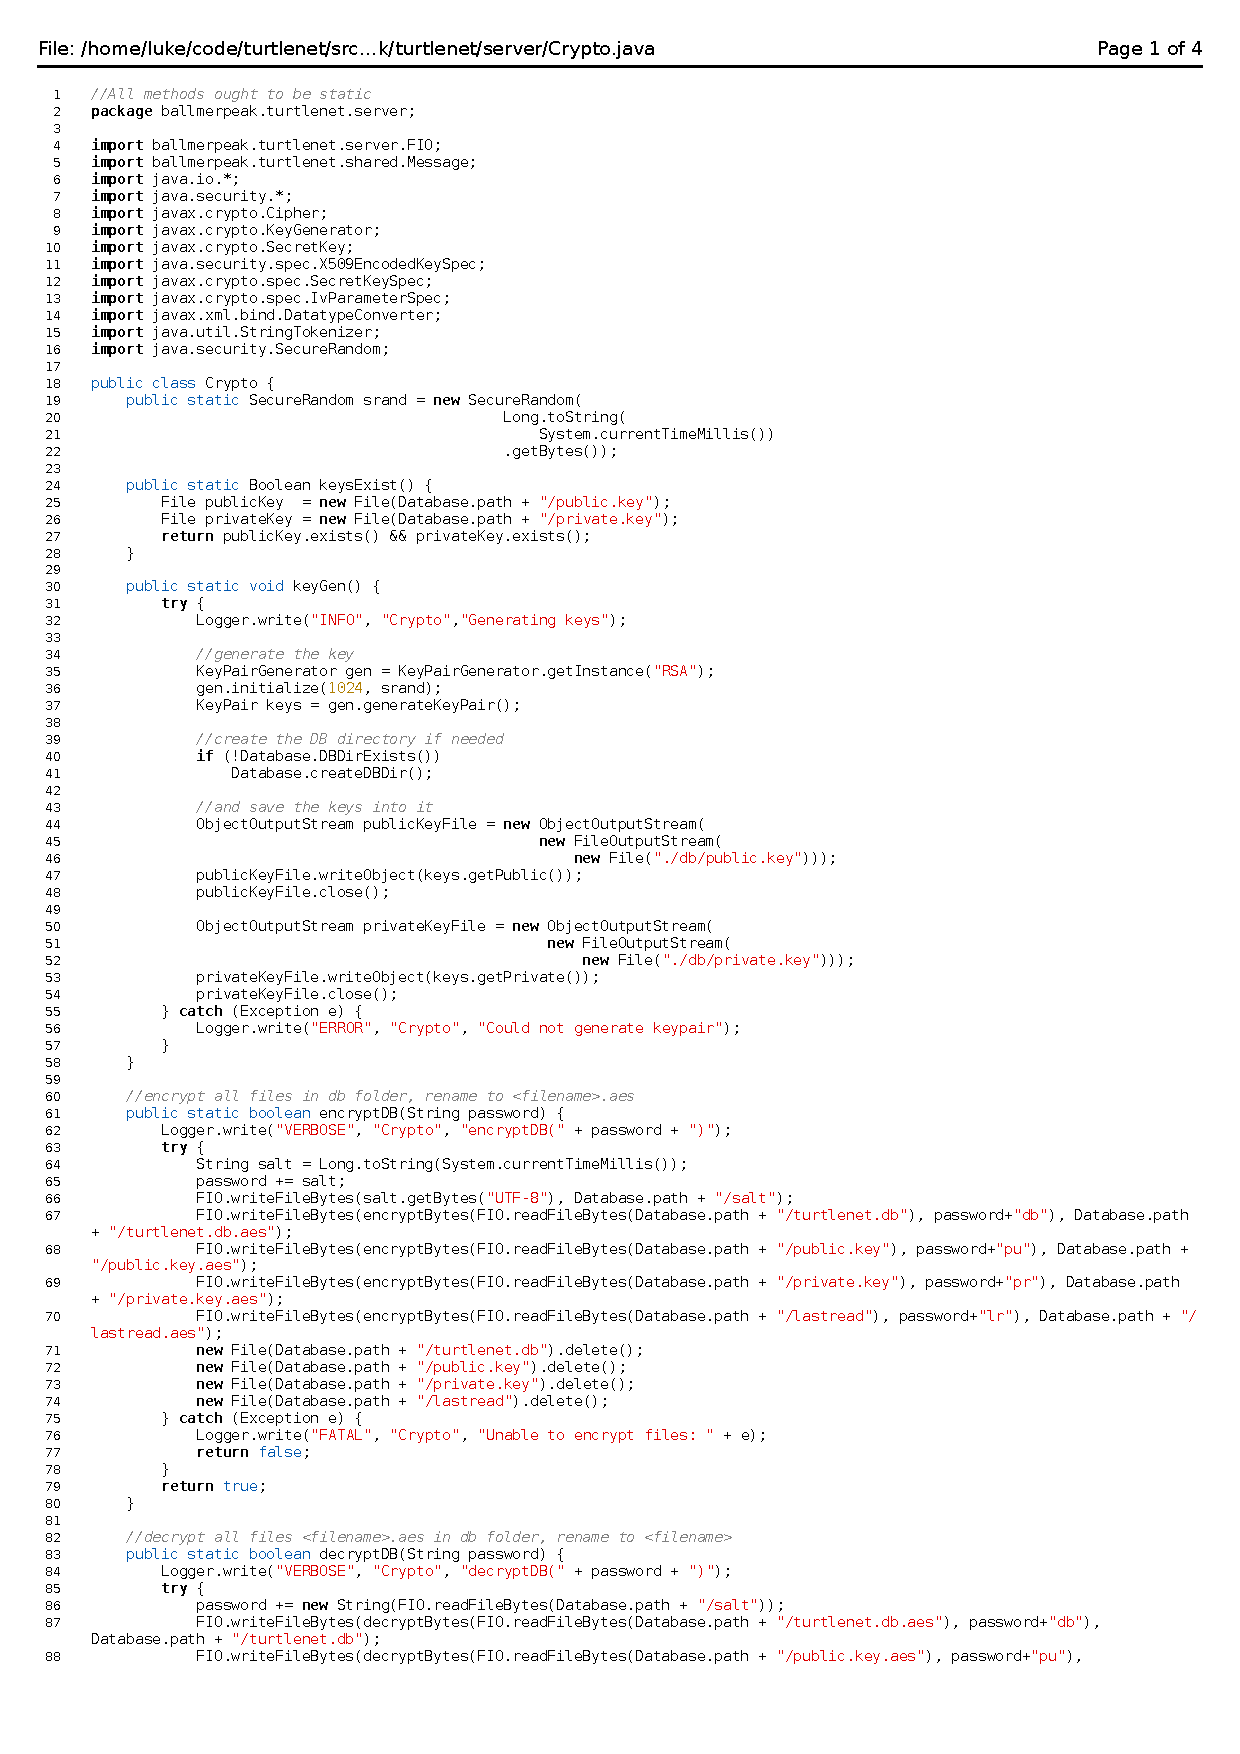
\includepdf[pages={-}]{./text/appendicies/source/8Crypto.pdf}
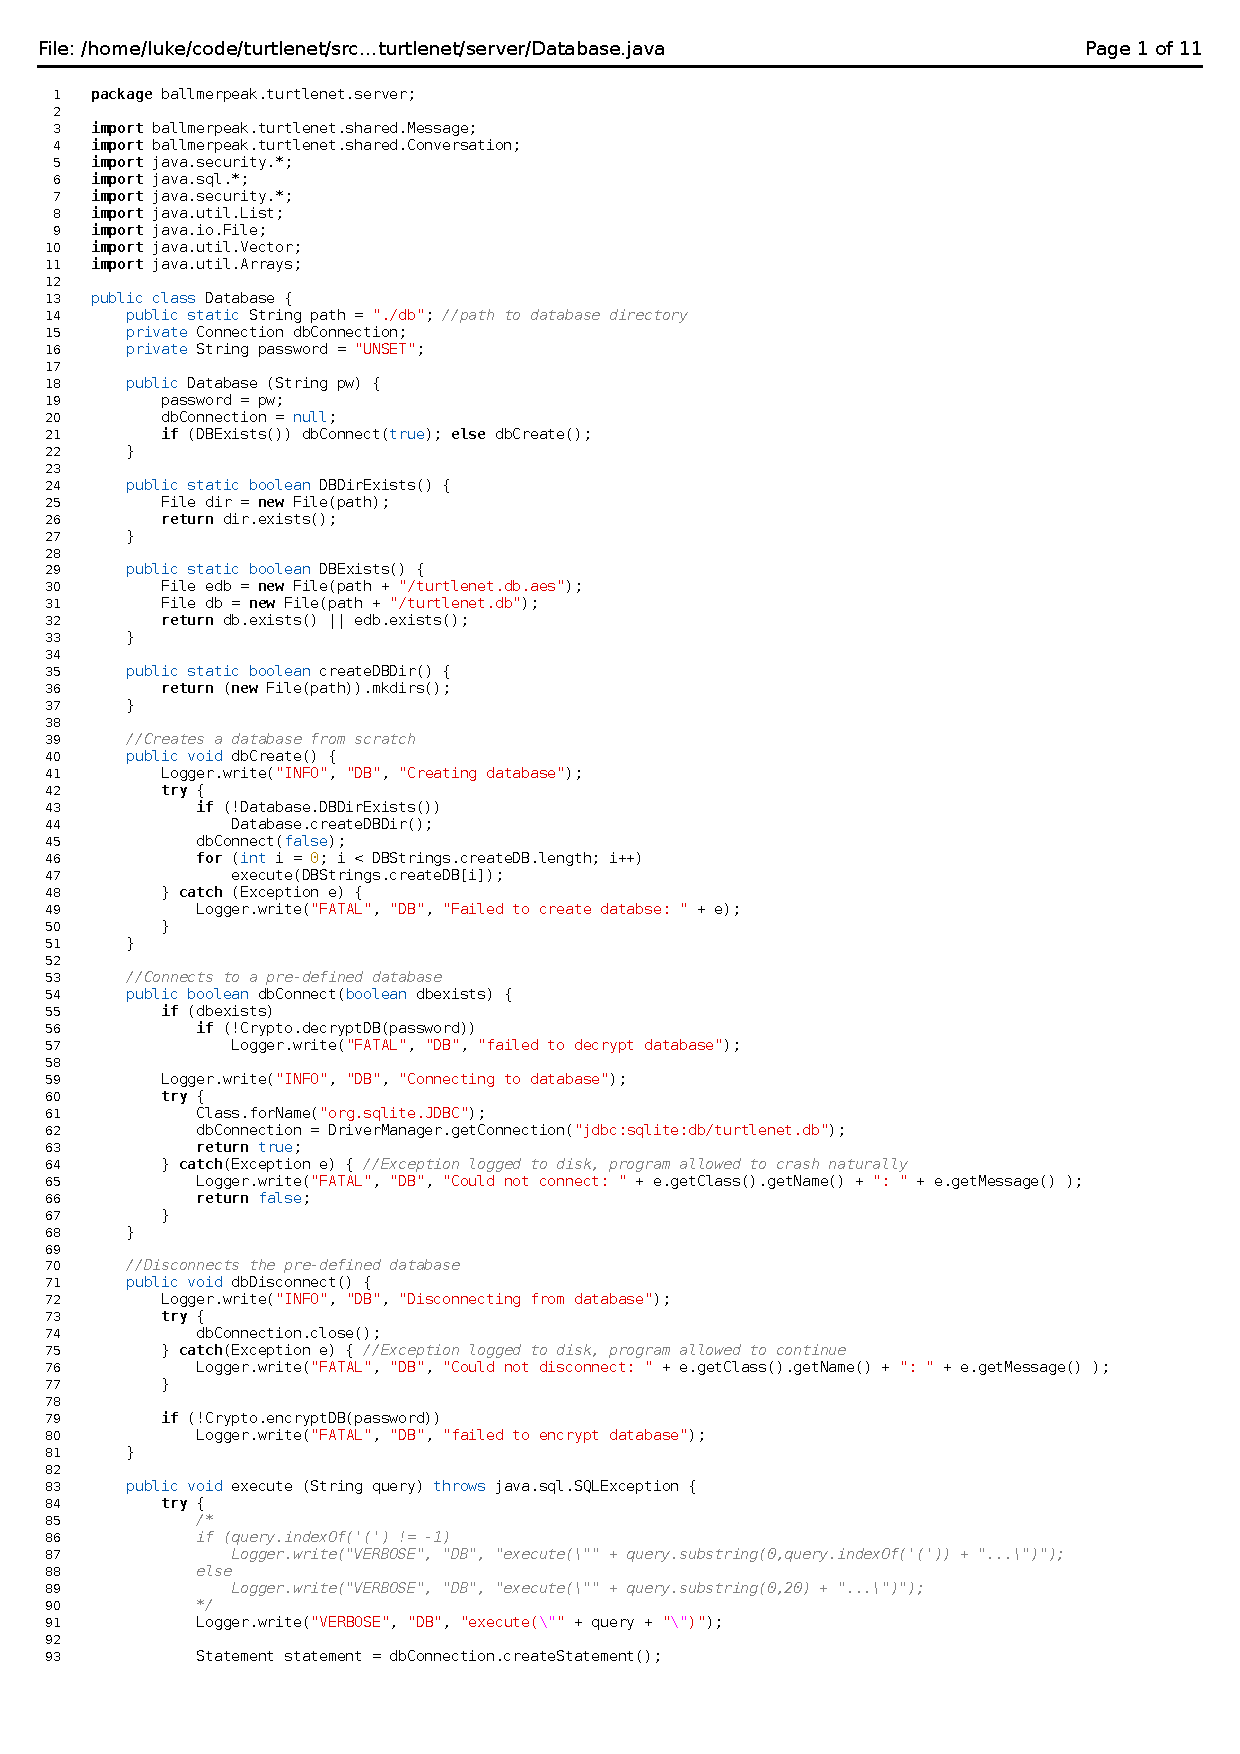
\includepdf[pages={-}]{./text/appendicies/source/9Database.pdf}
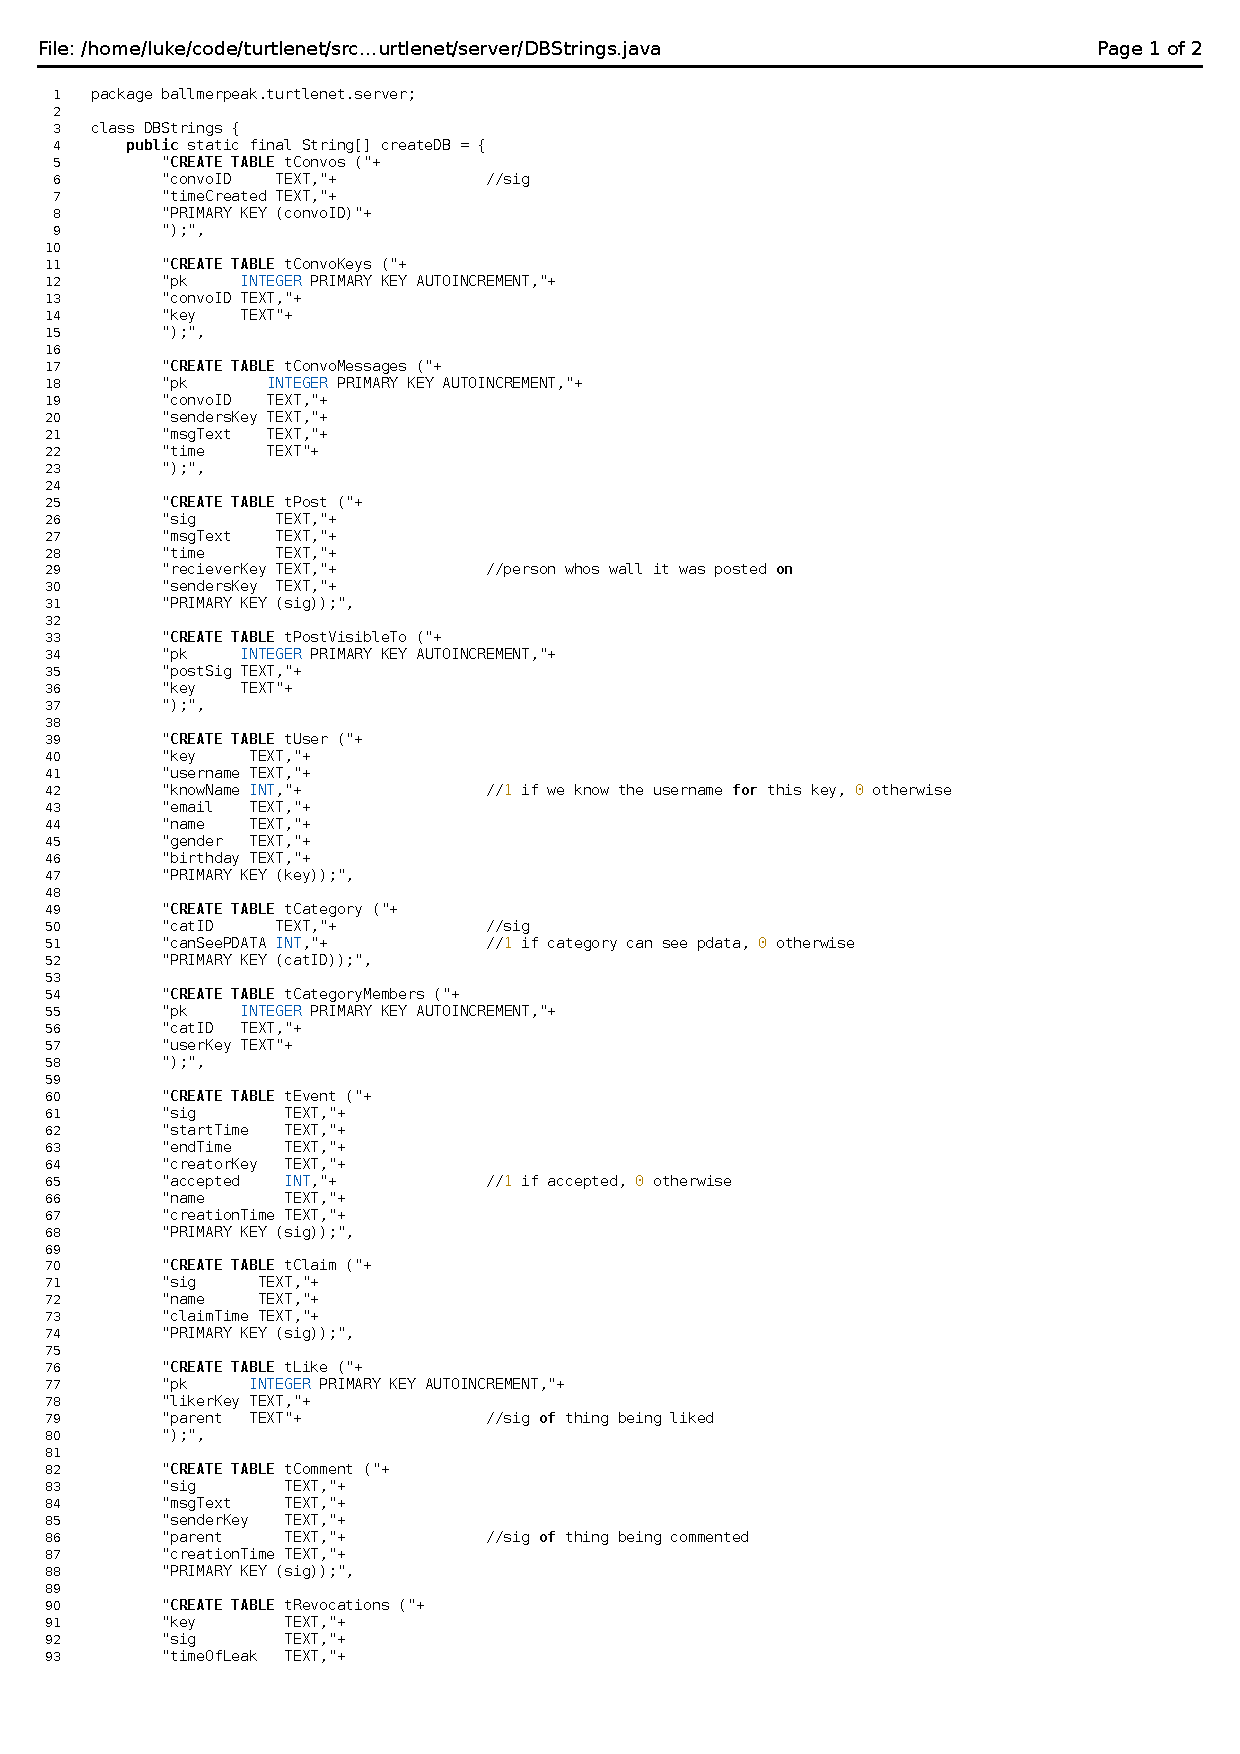
\includepdf[pages={-}]{./text/appendicies/source/10DBStrings.pdf}
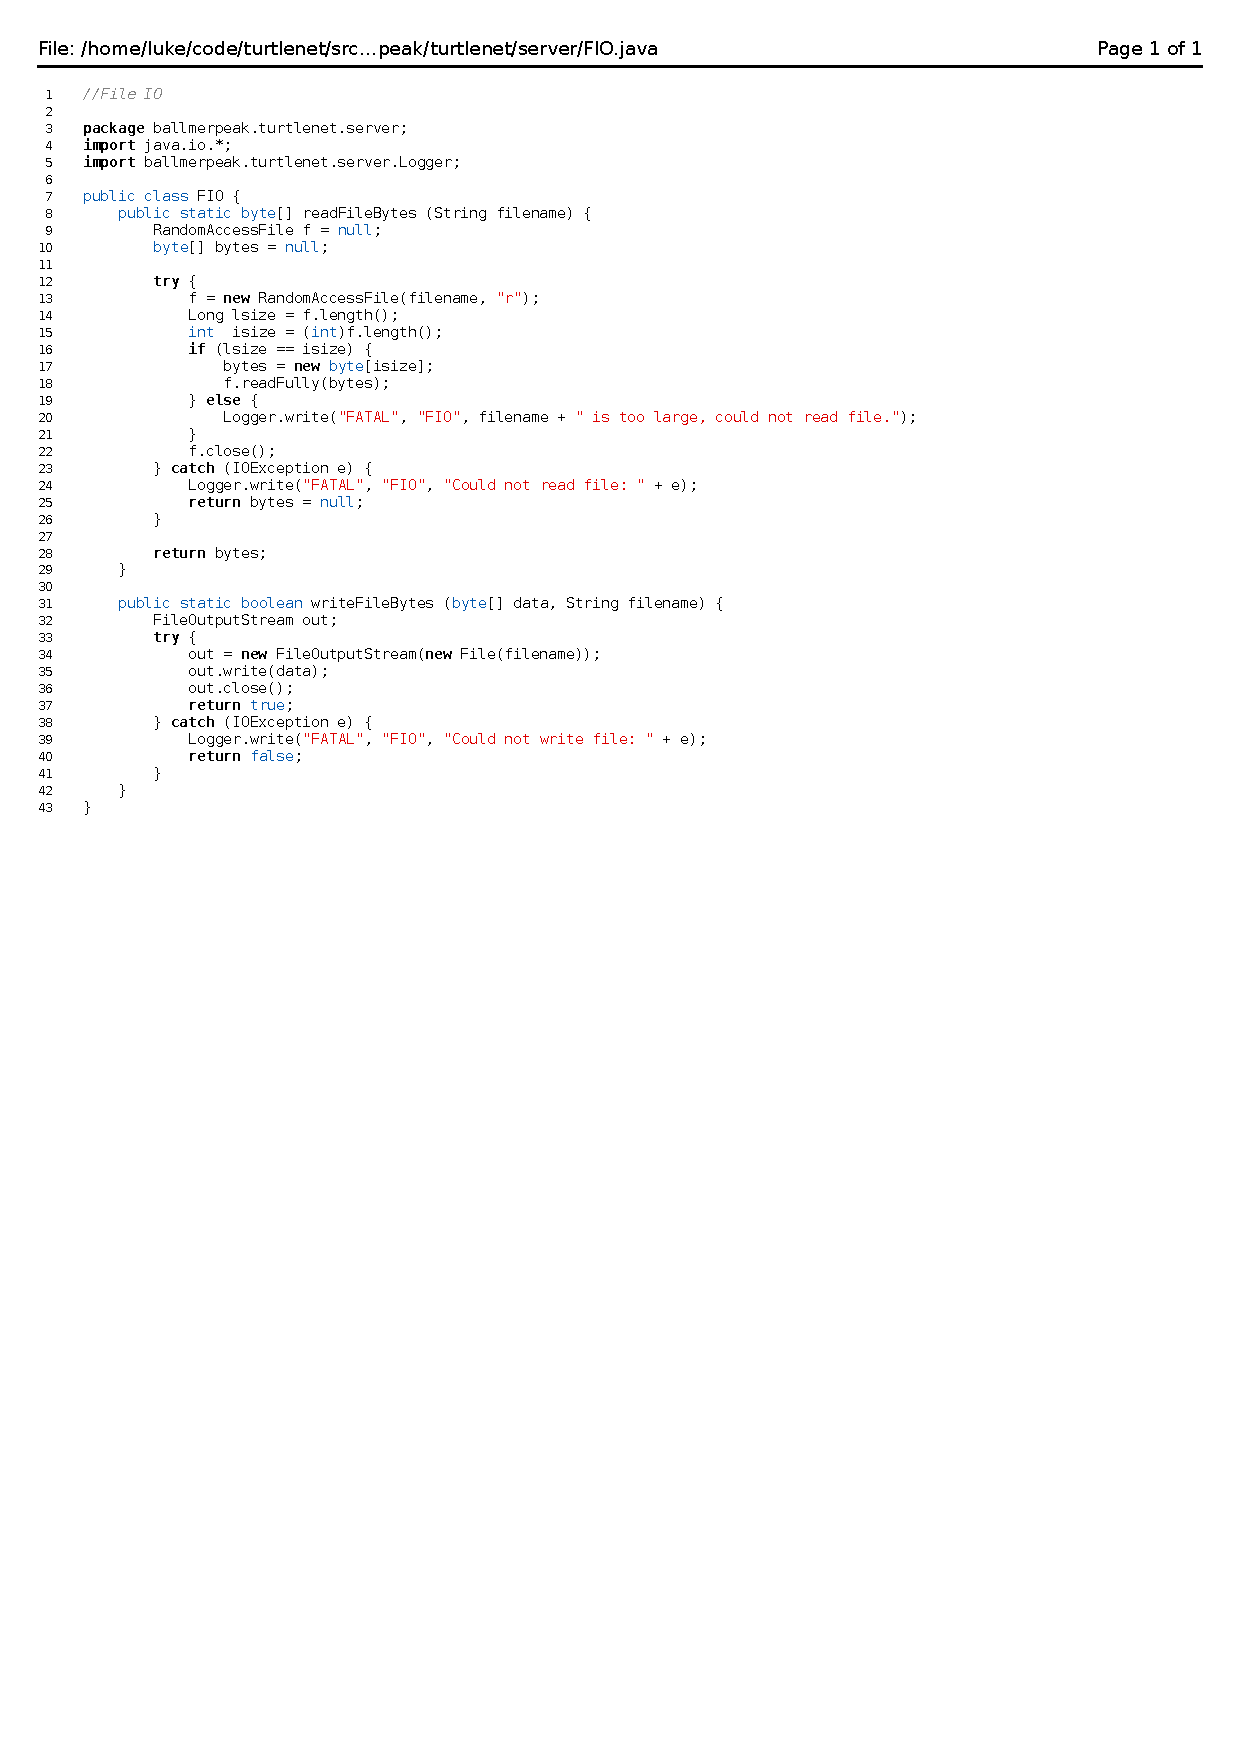
\includepdf[pages={-}]{./text/appendicies/source/11FIO.pdf}
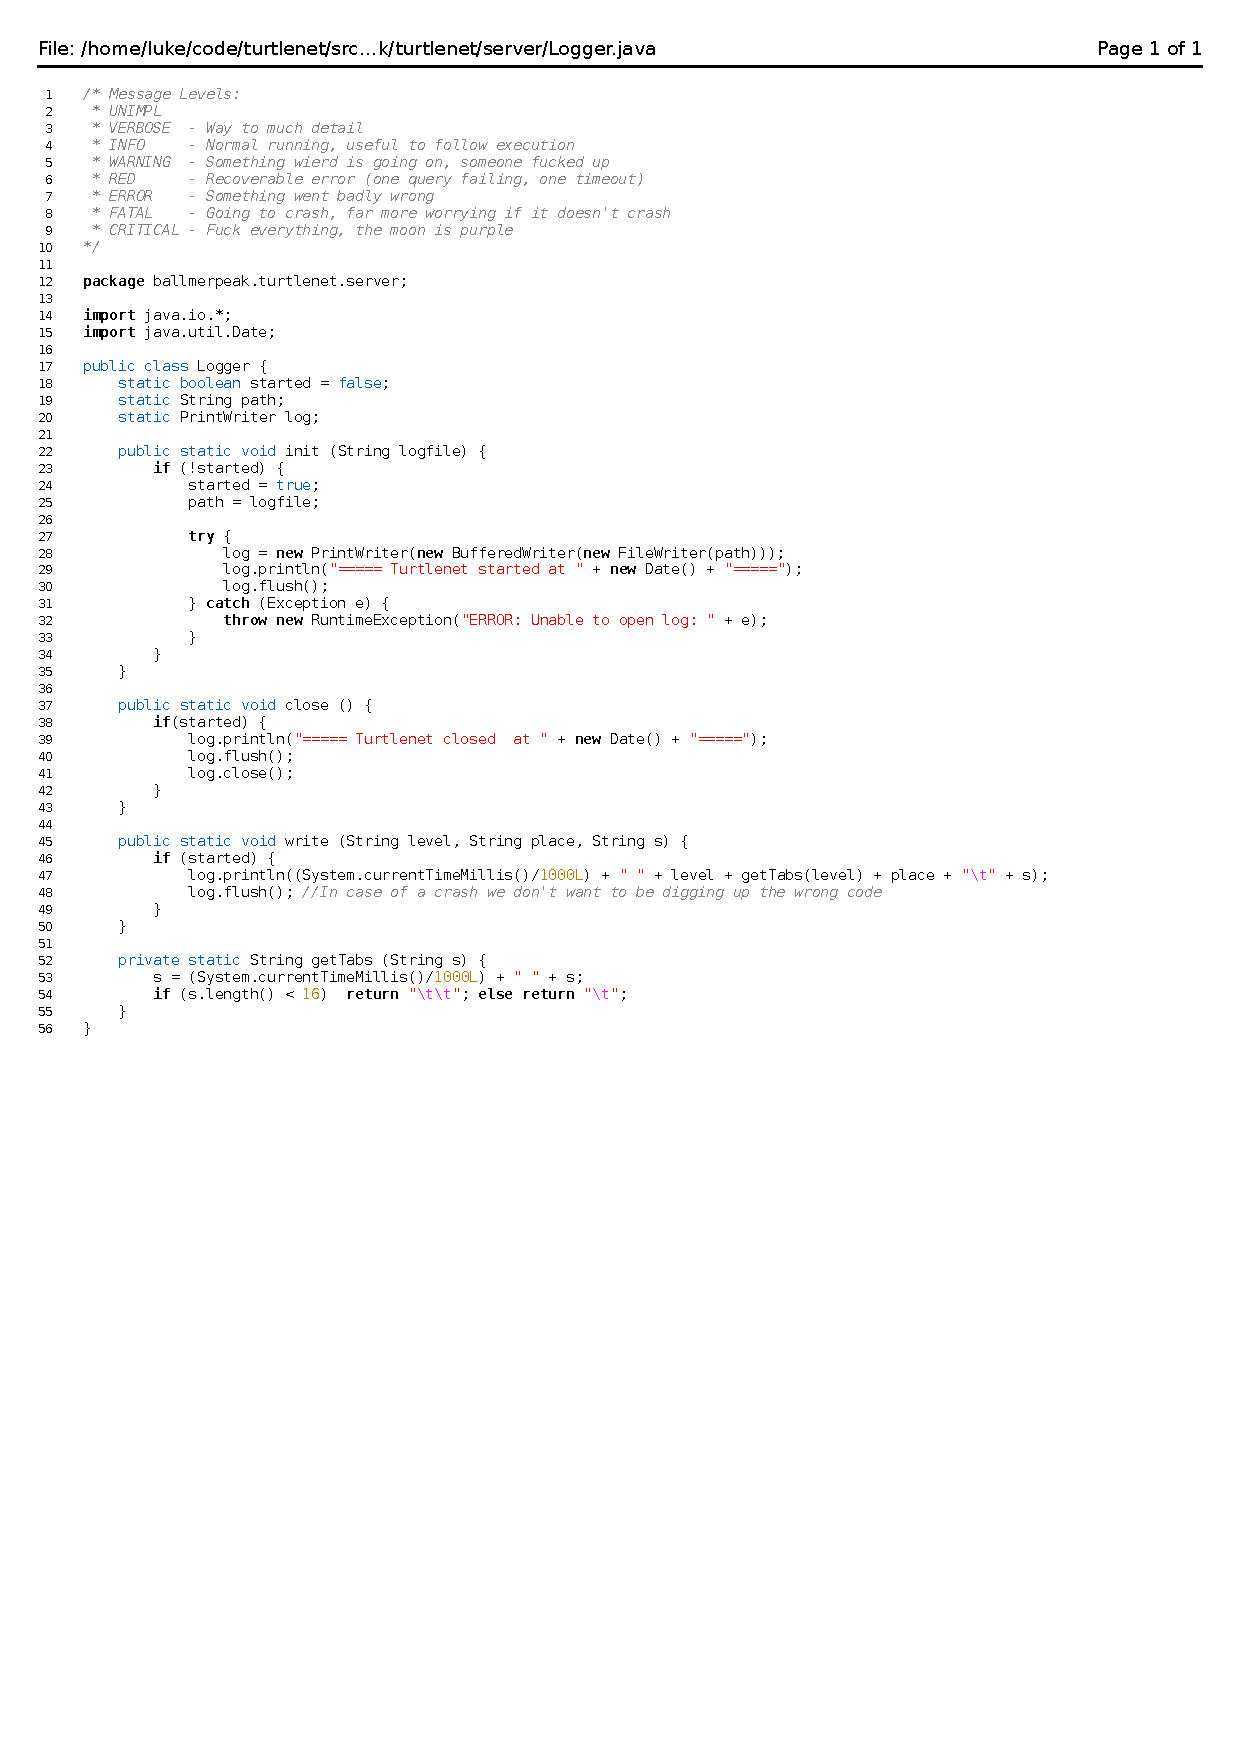
\includepdf[pages={-}]{./text/appendicies/source/12Logger.pdf}
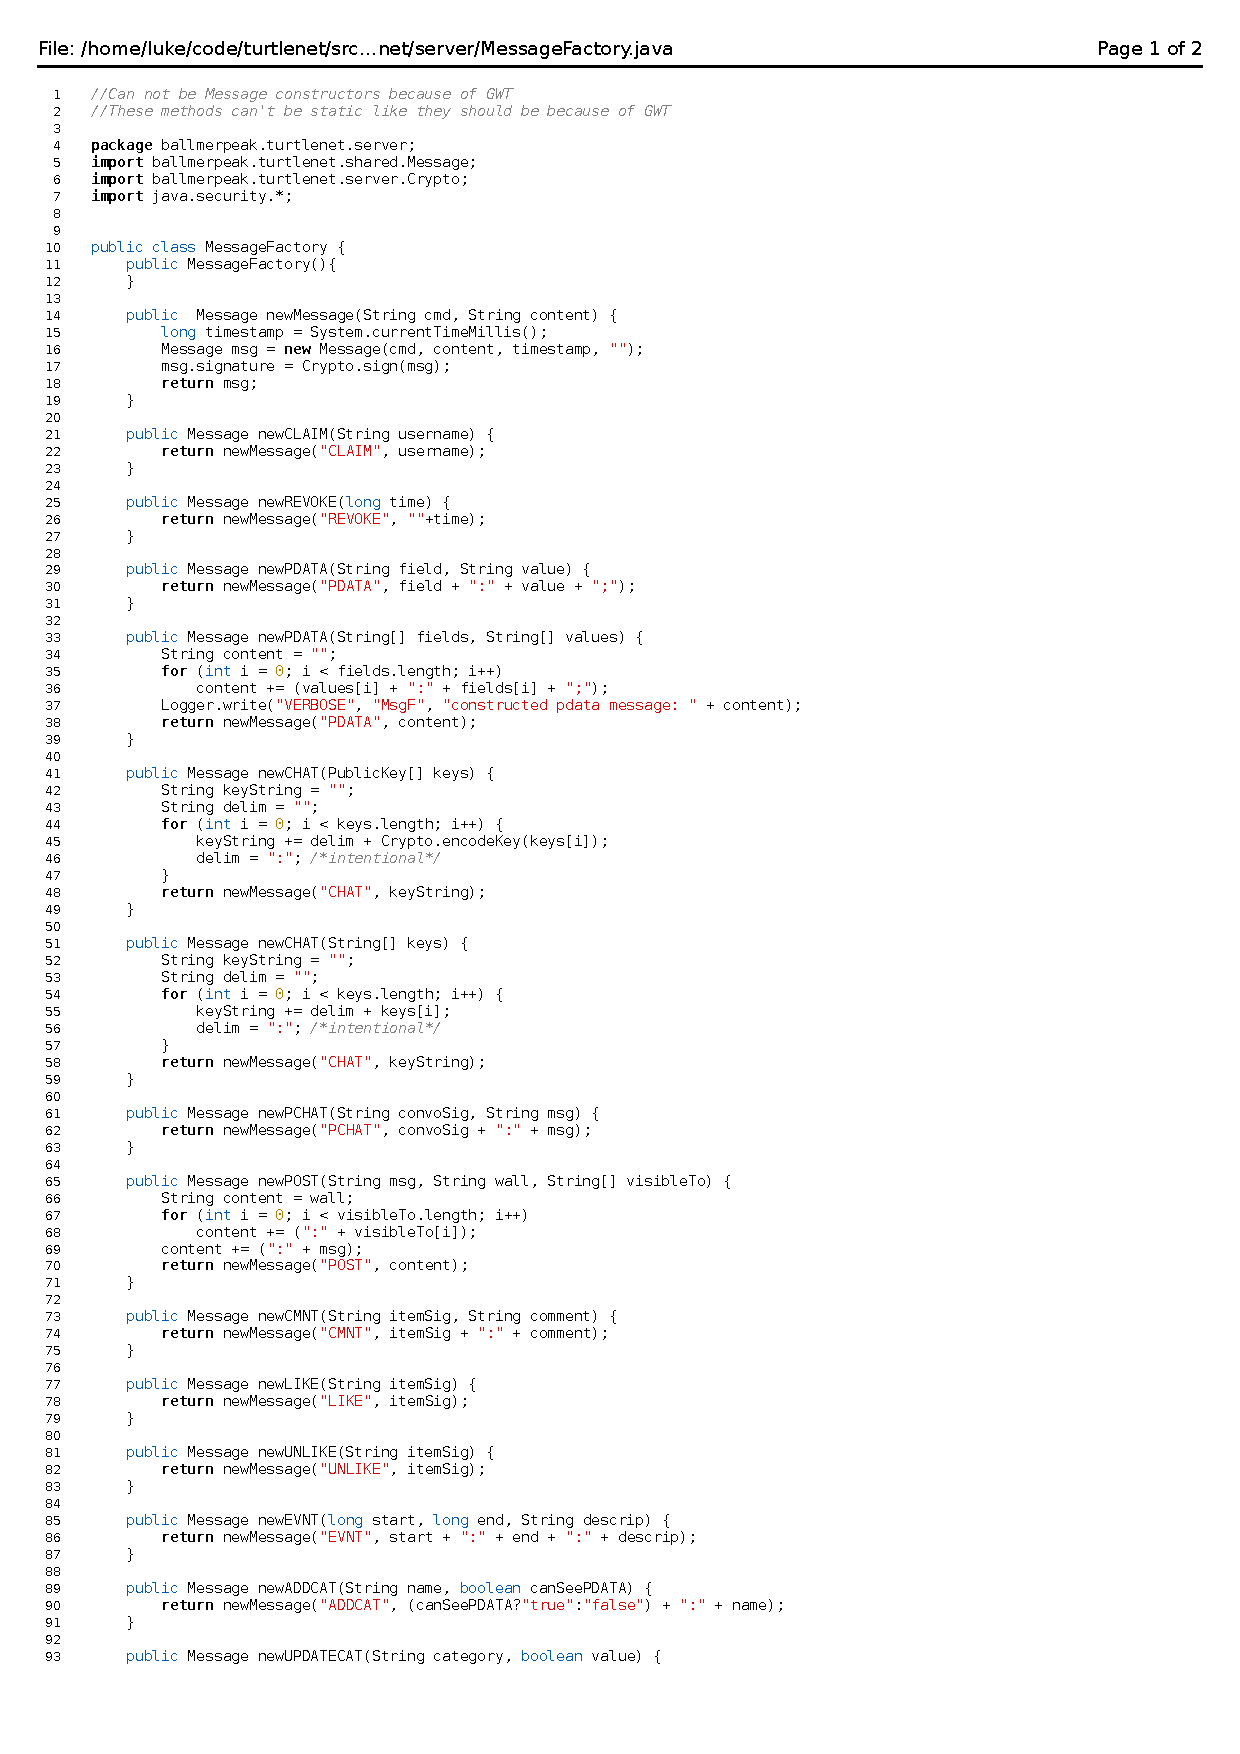
\includepdf[pages={-}]{./text/appendicies/source/13MessageFactory.pdf}
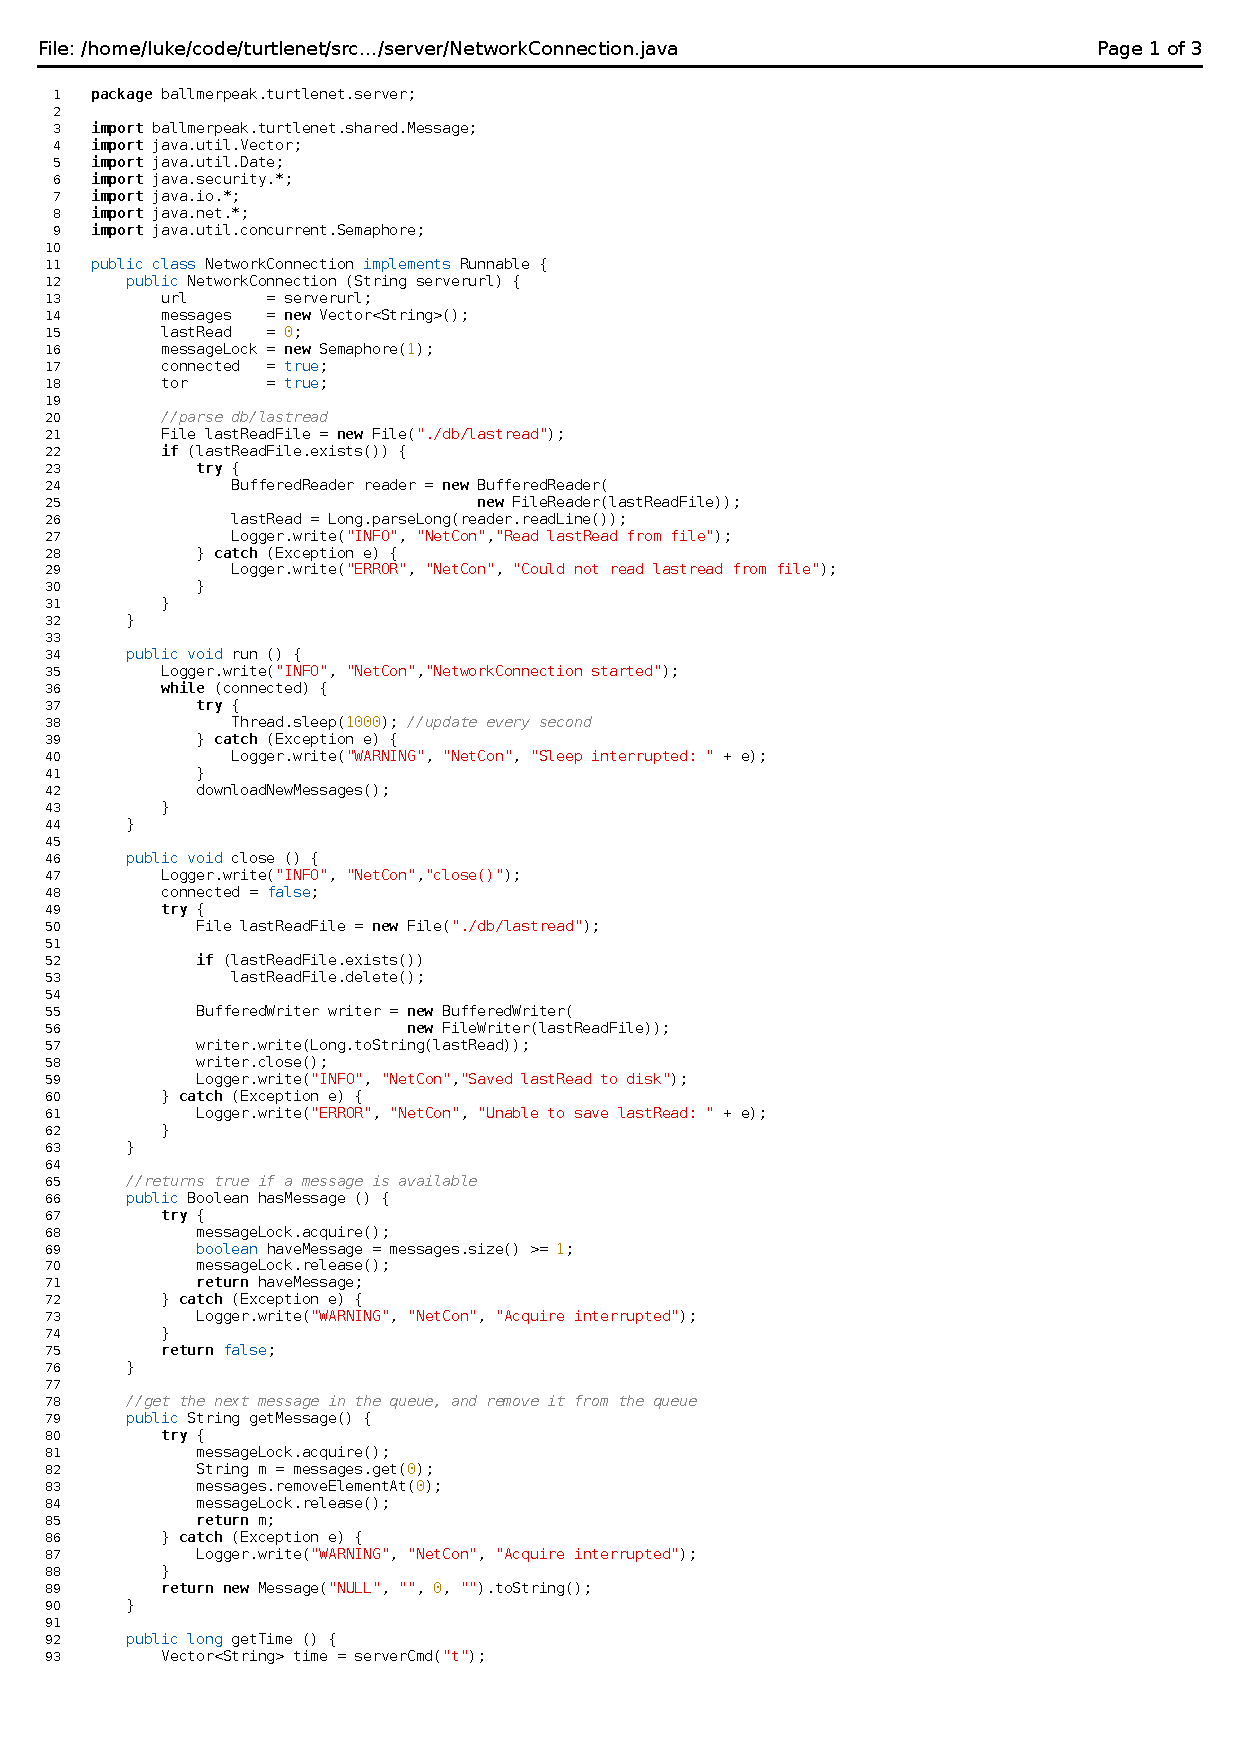
\includepdf[pages={-}]{./text/appendicies/source/14NetworkConnection.pdf}
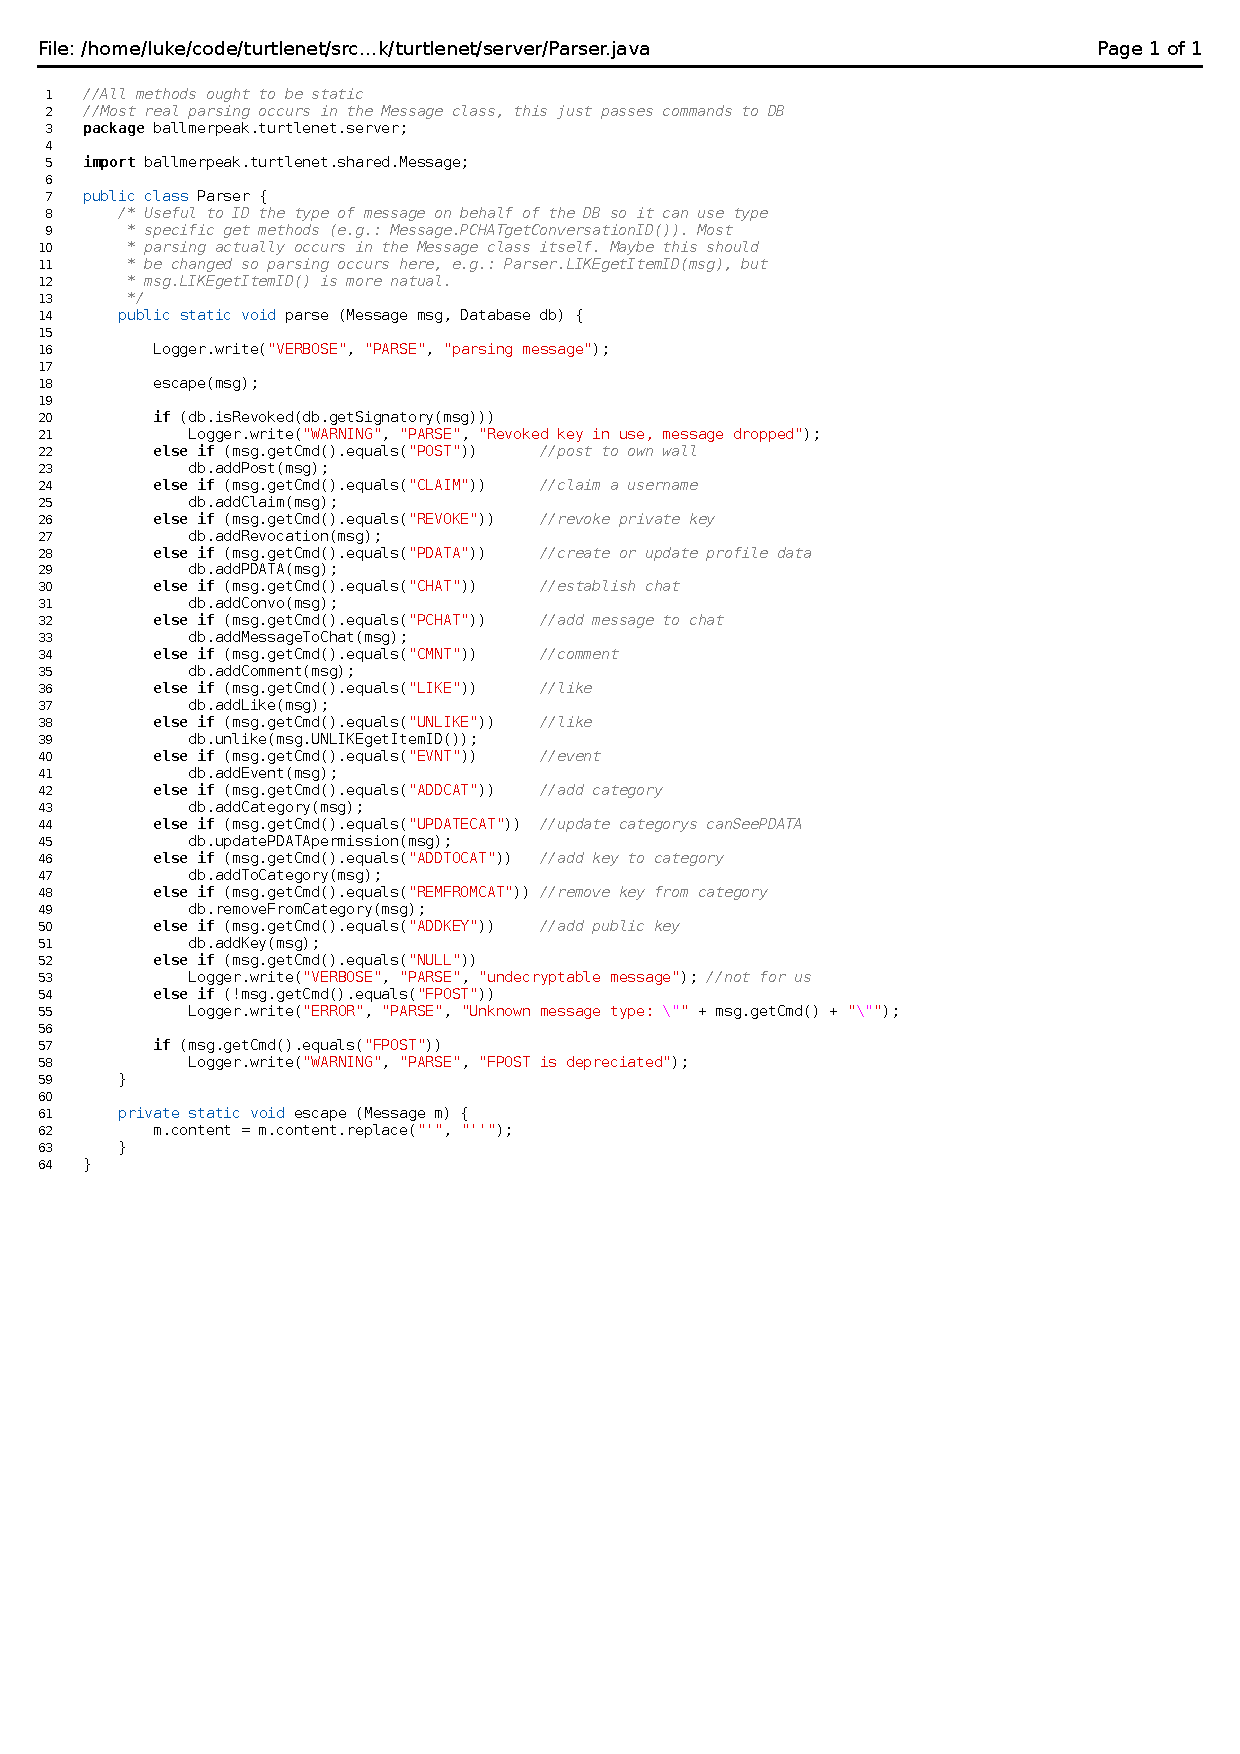
\includepdf[pages={-}]{./text/appendicies/source/15Parser.pdf}
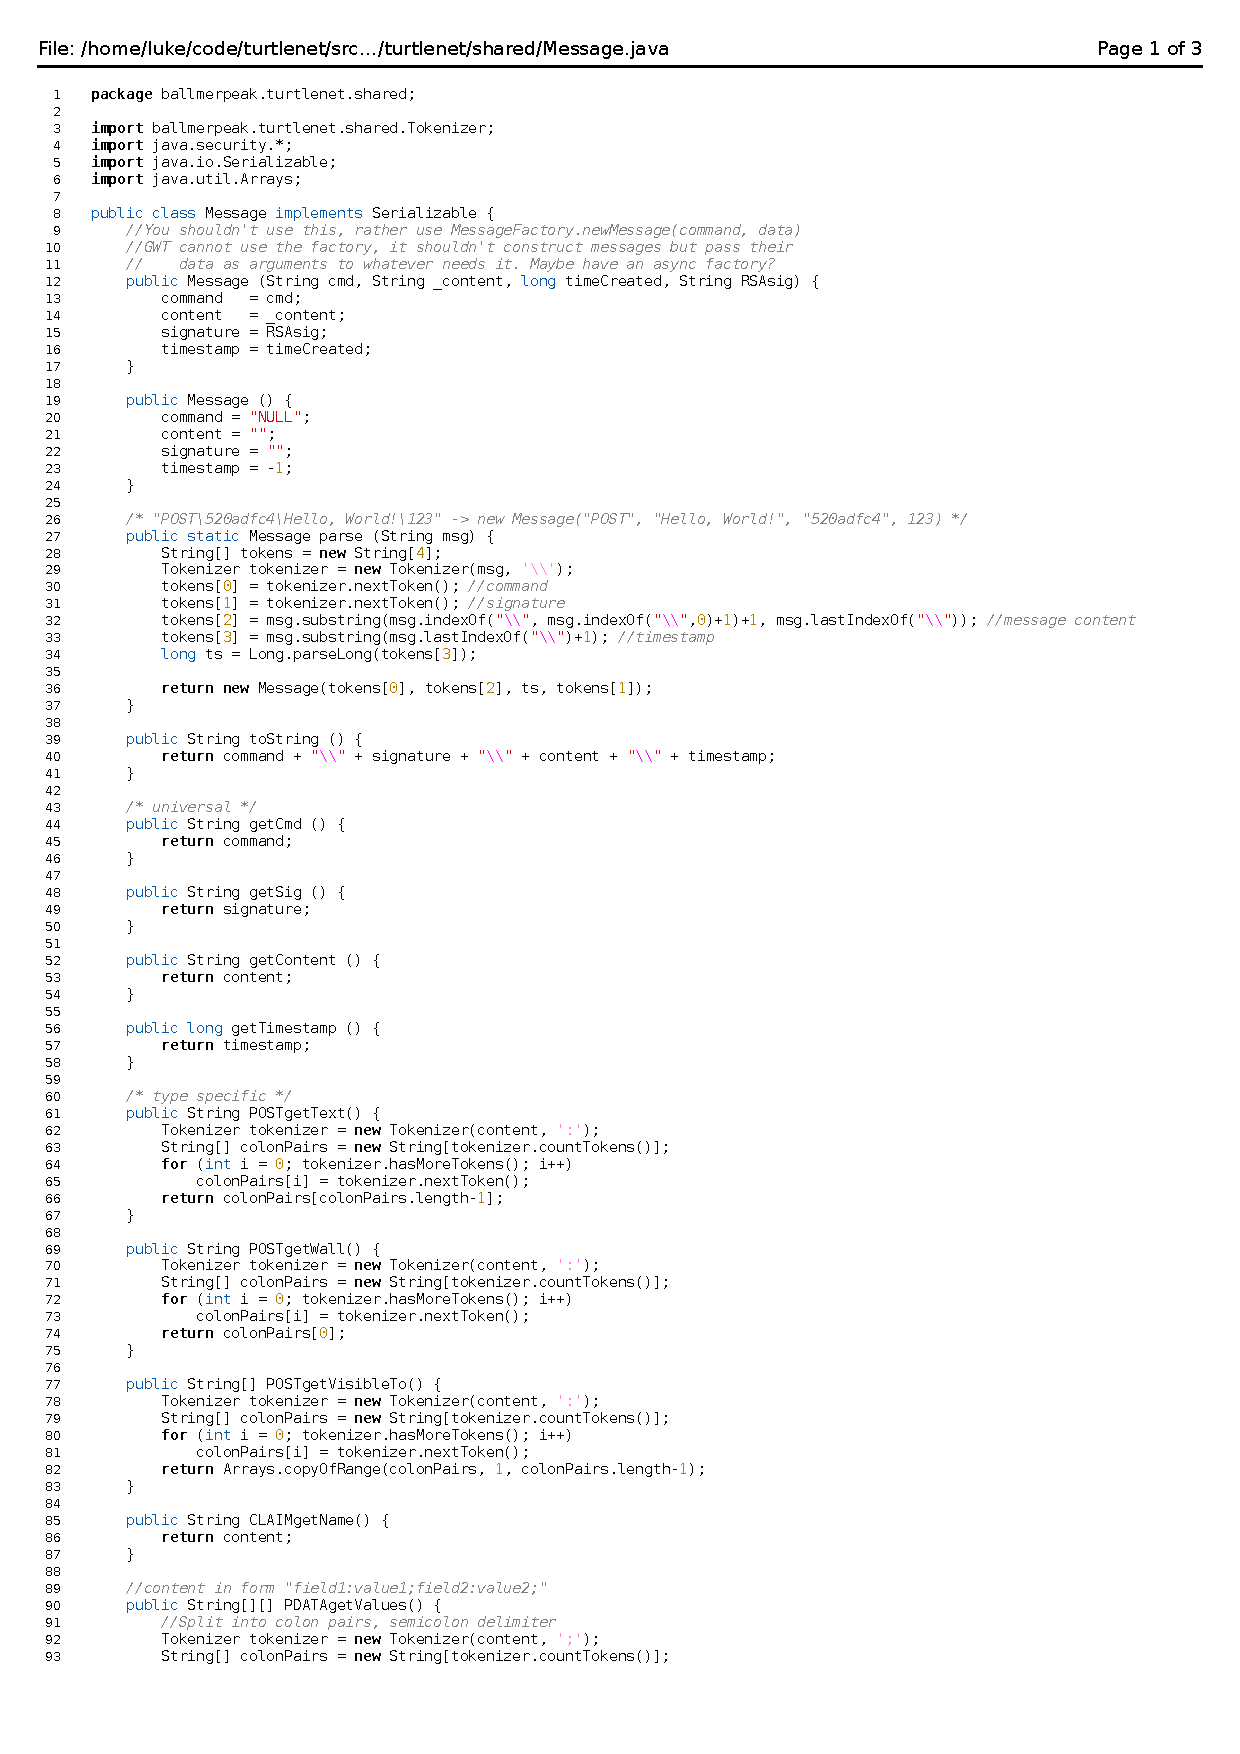
\includepdf[pages={-}]{./text/appendicies/source/16Message.pdf}
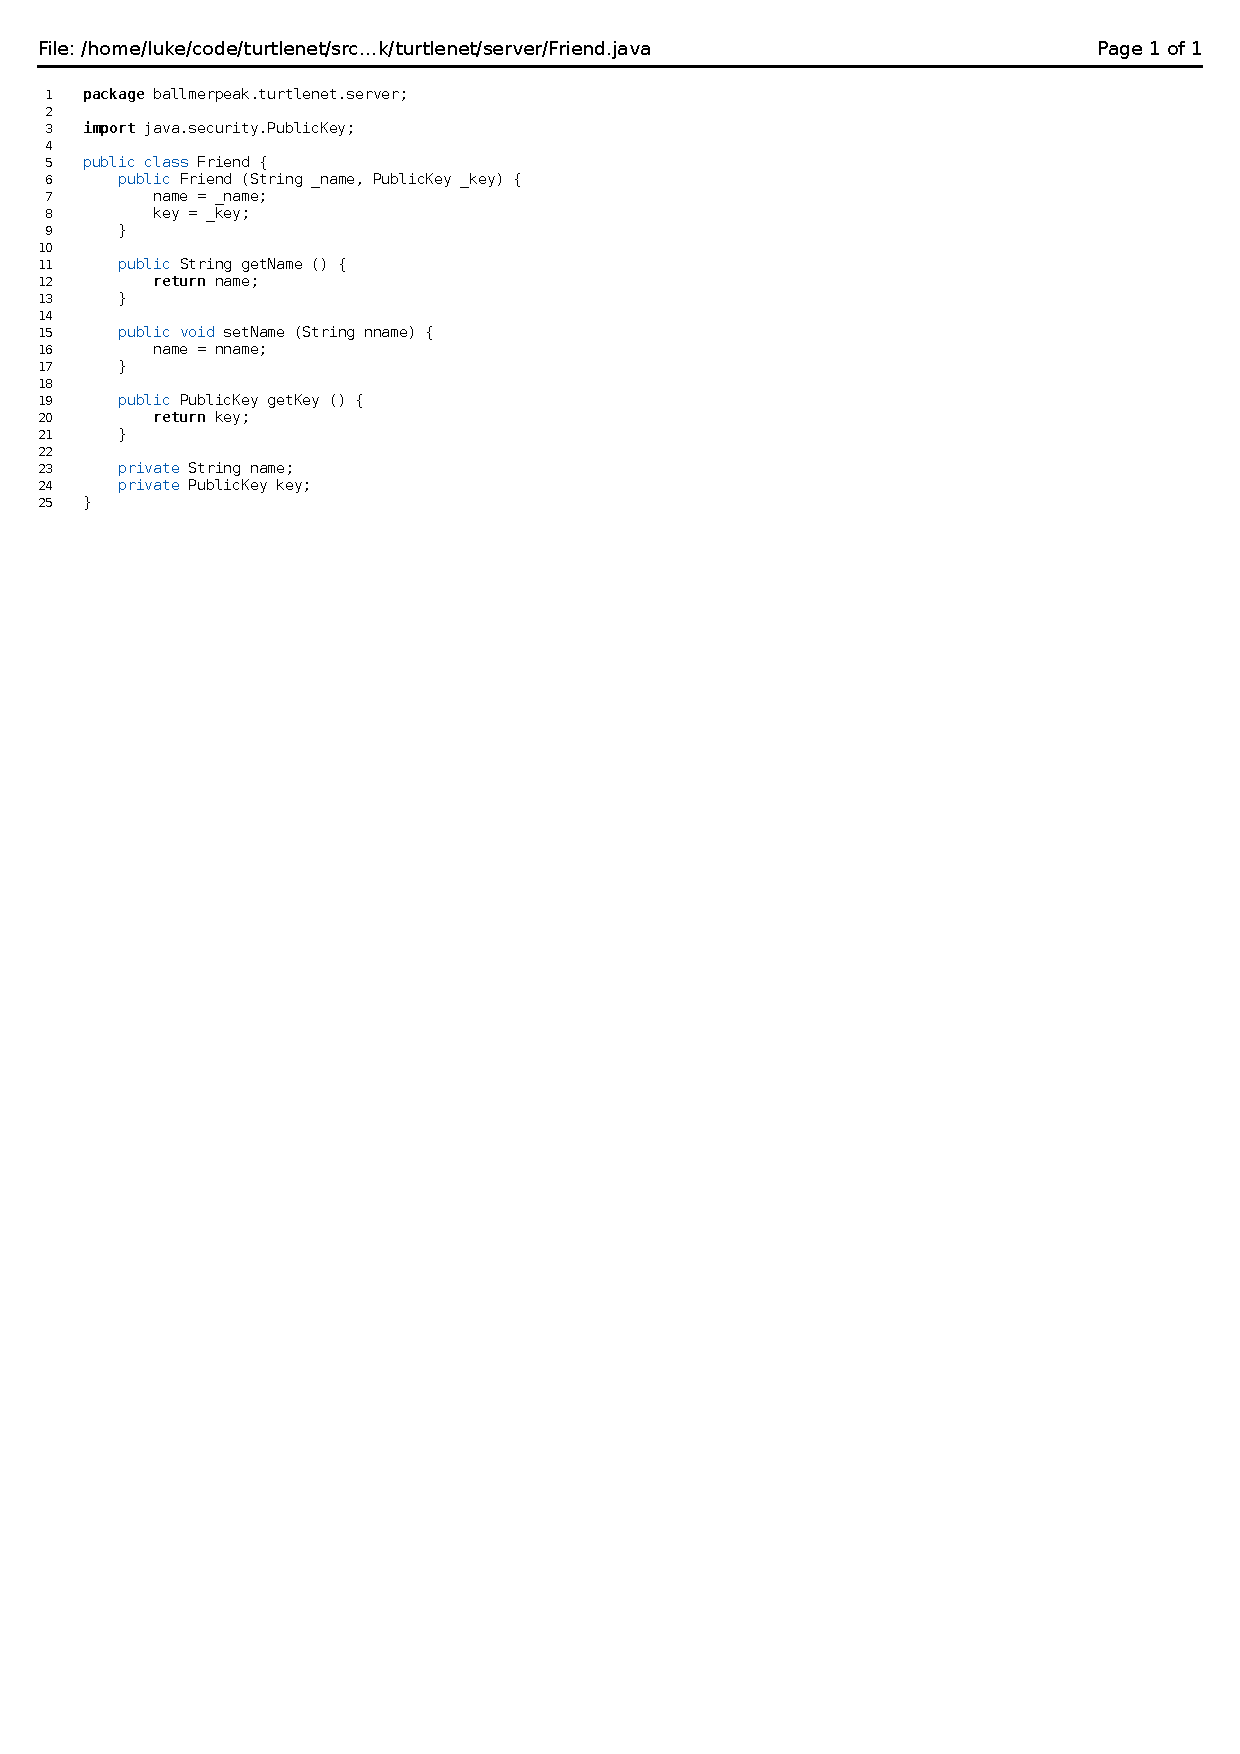
\includepdf[pages={-}]{./text/appendicies/source/17Friend.pdf}
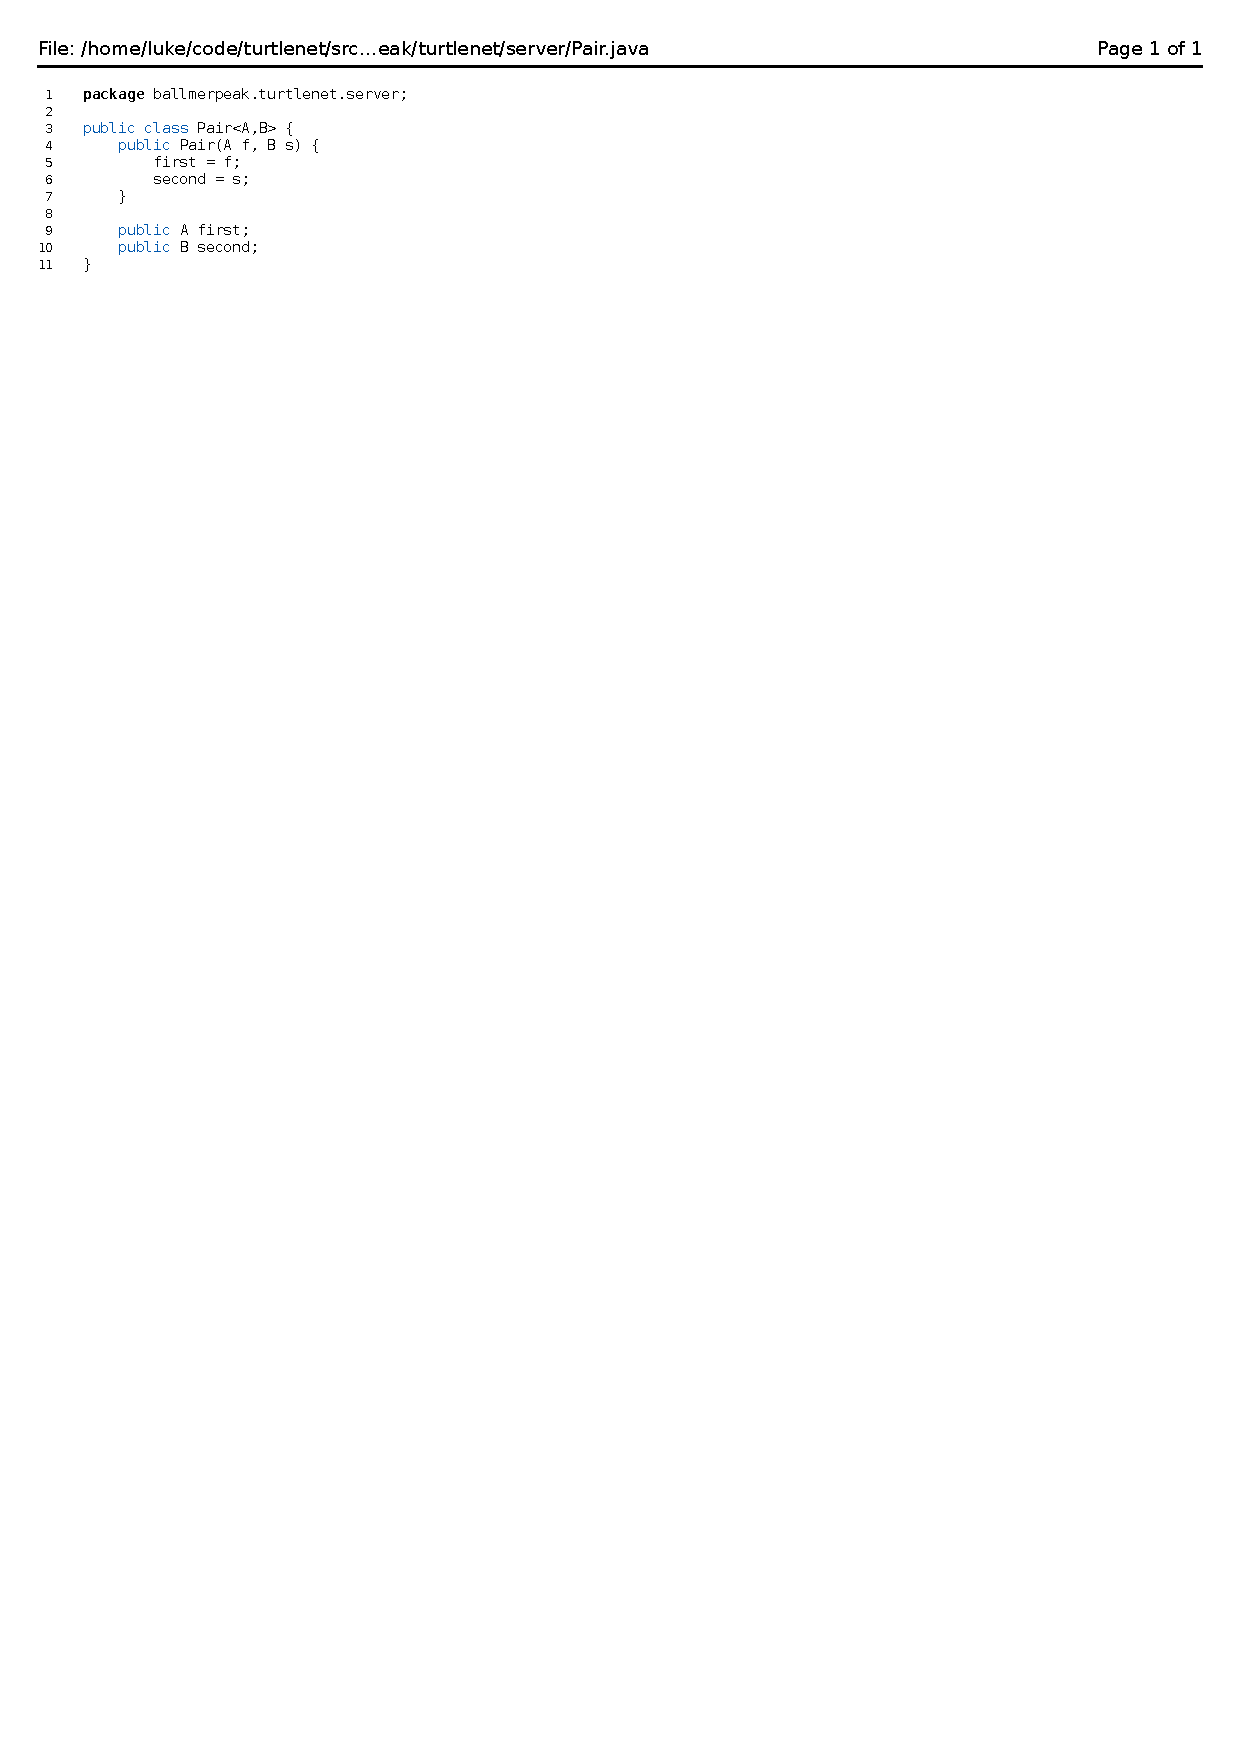
\includepdf[pages={-}]{./text/appendicies/source/18Pair.pdf}
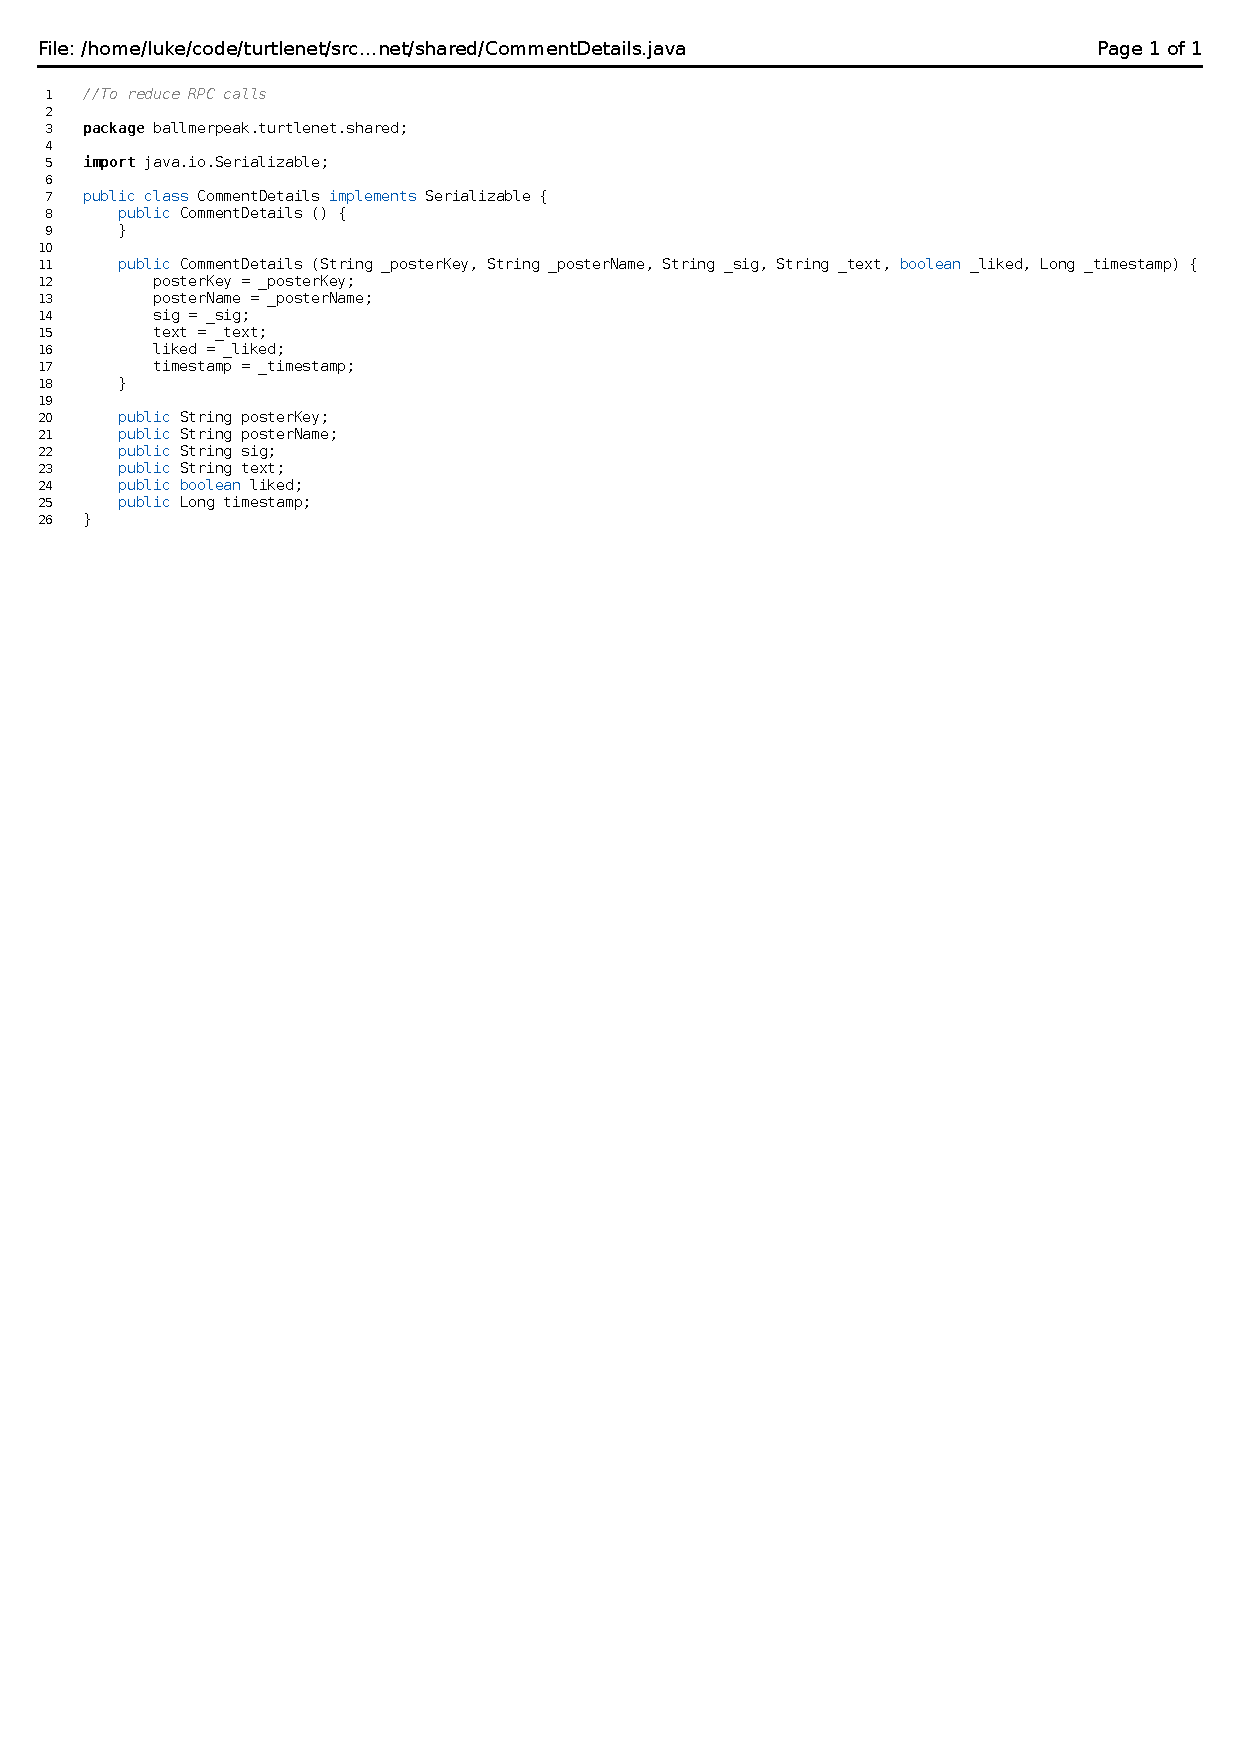
\includepdf[pages={-}]{./text/appendicies/source/19CommentDetails.pdf}
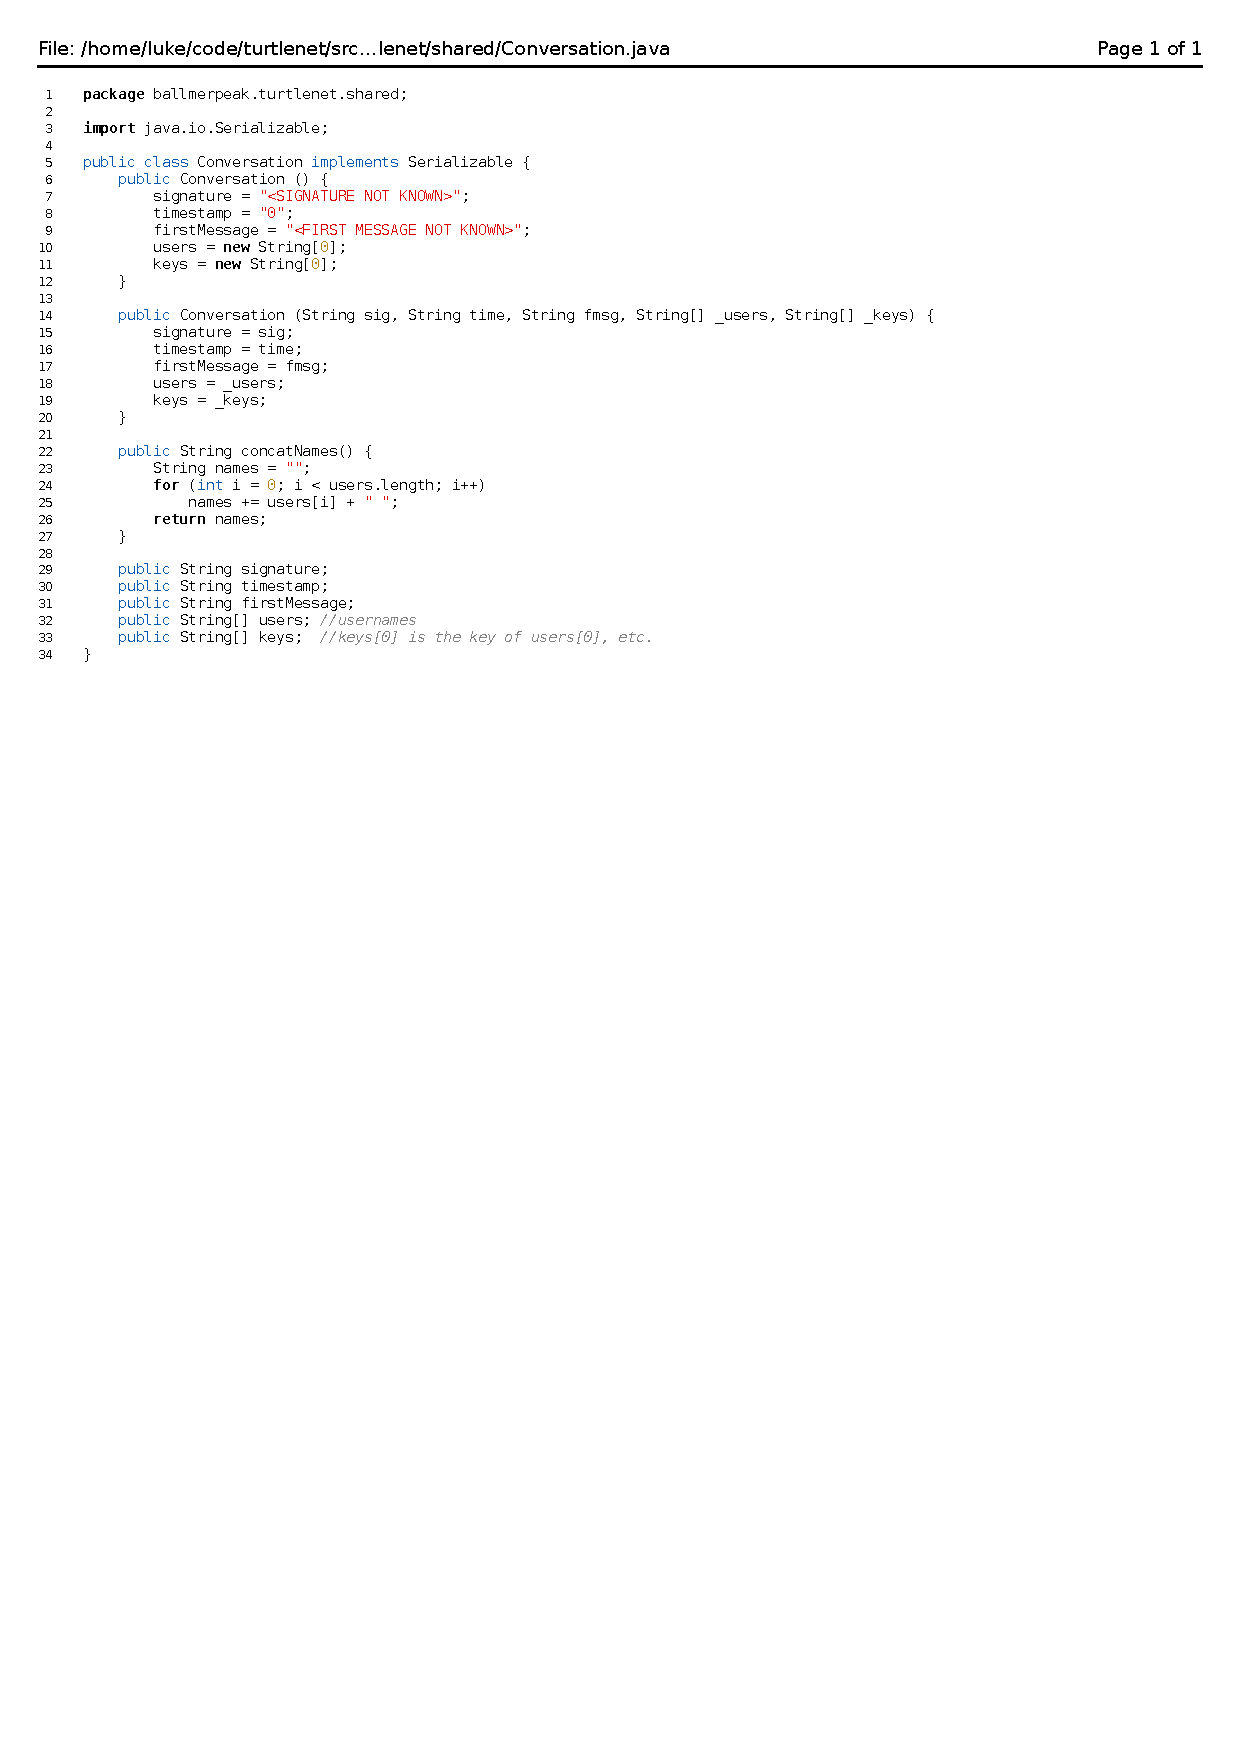
\includepdf[pages={-}]{./text/appendicies/source/20Conversation.pdf}
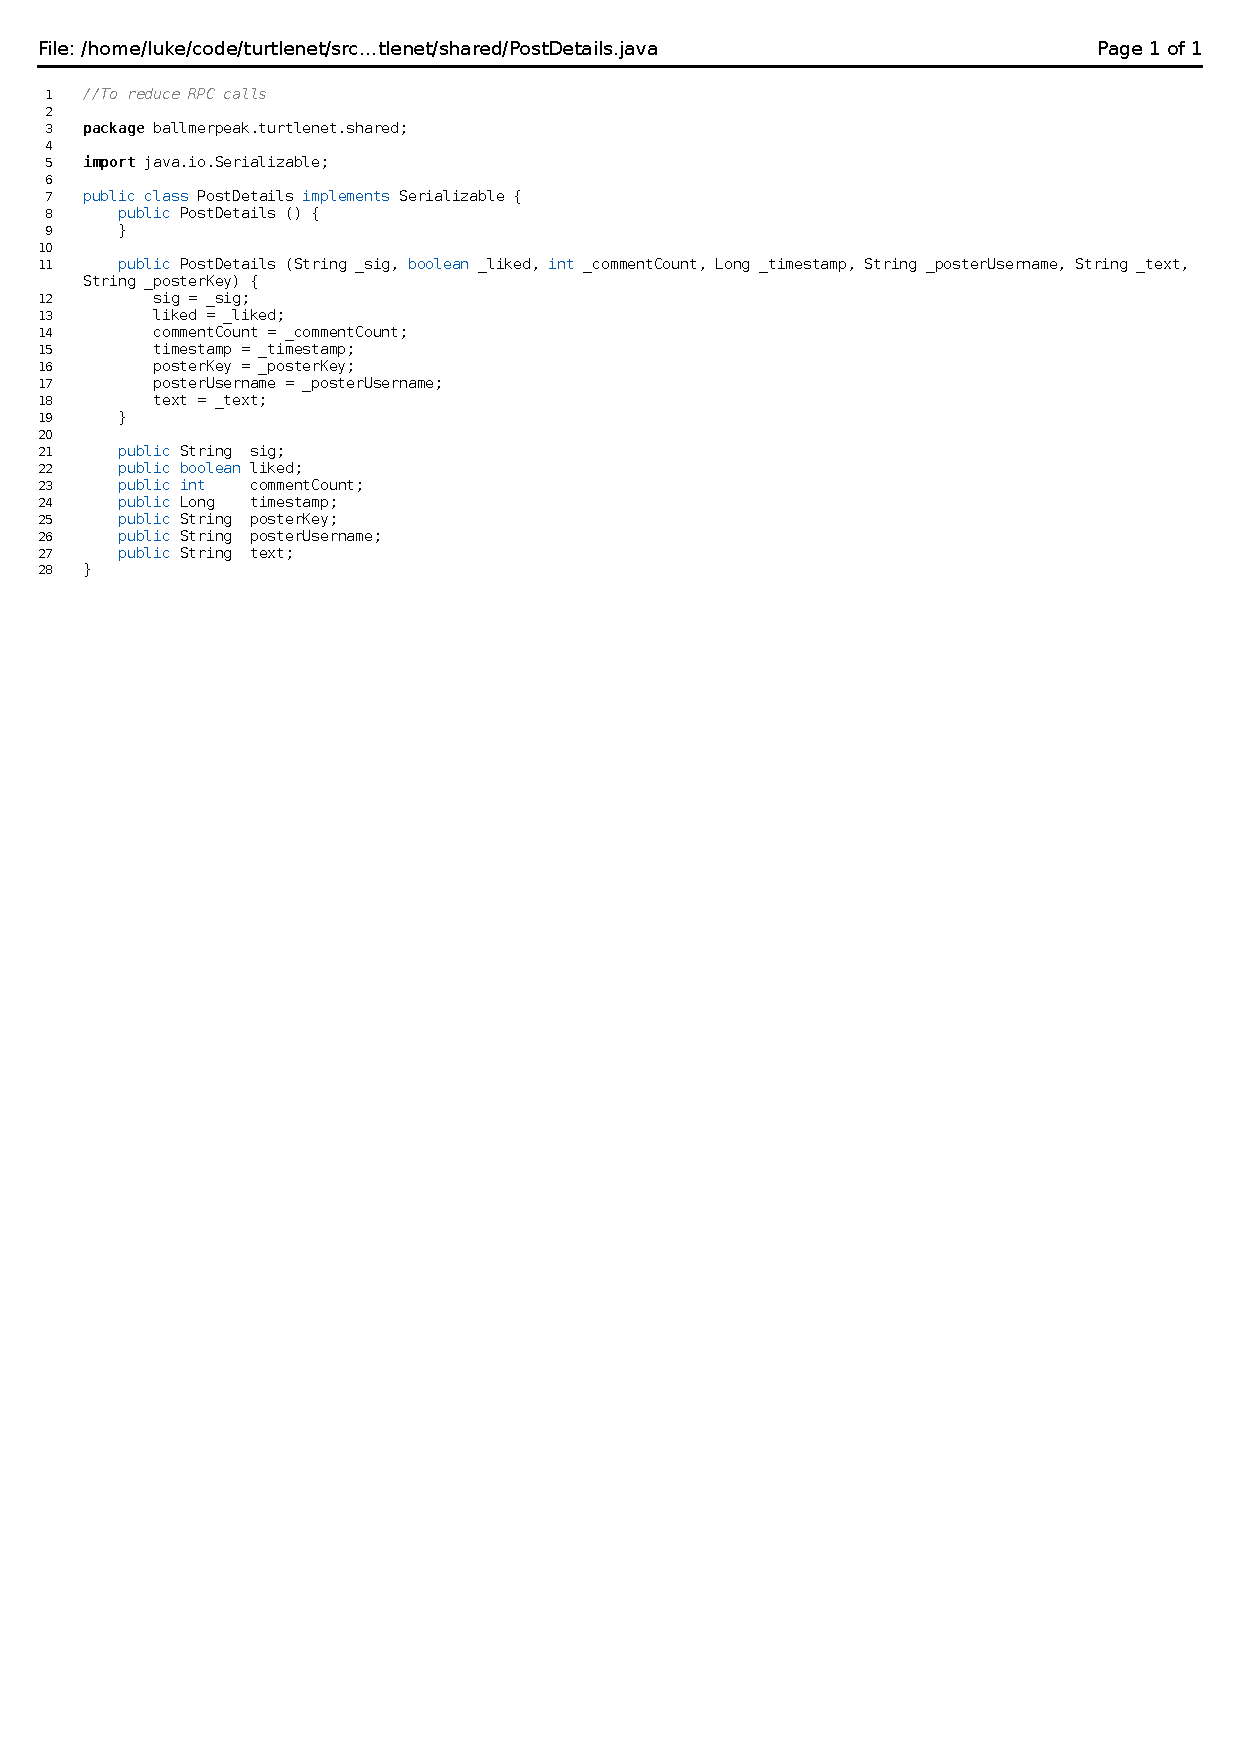
\includepdf[pages={-}]{./text/appendicies/source/21PostDetails.pdf}
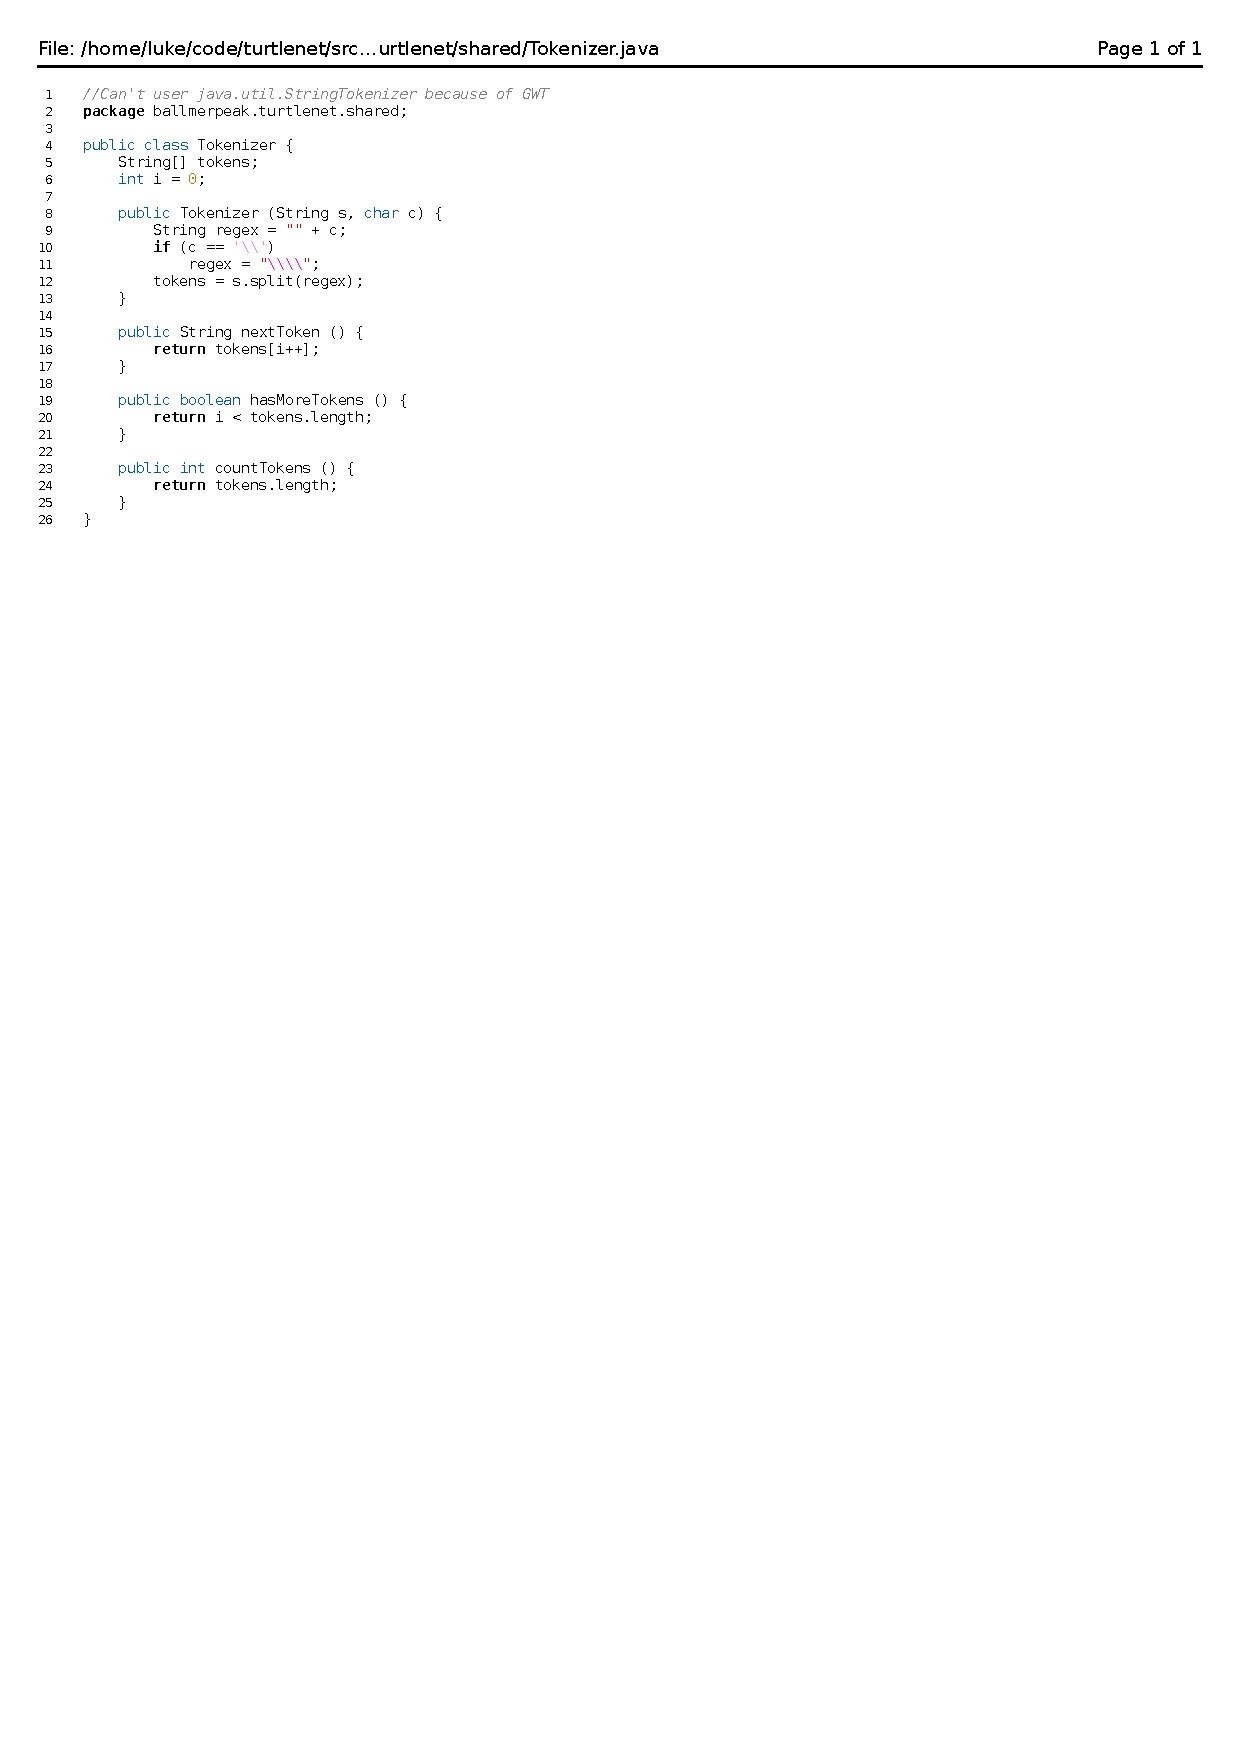
\includepdf[pages={-}]{./text/appendicies/source/22Tokenizer.pdf}
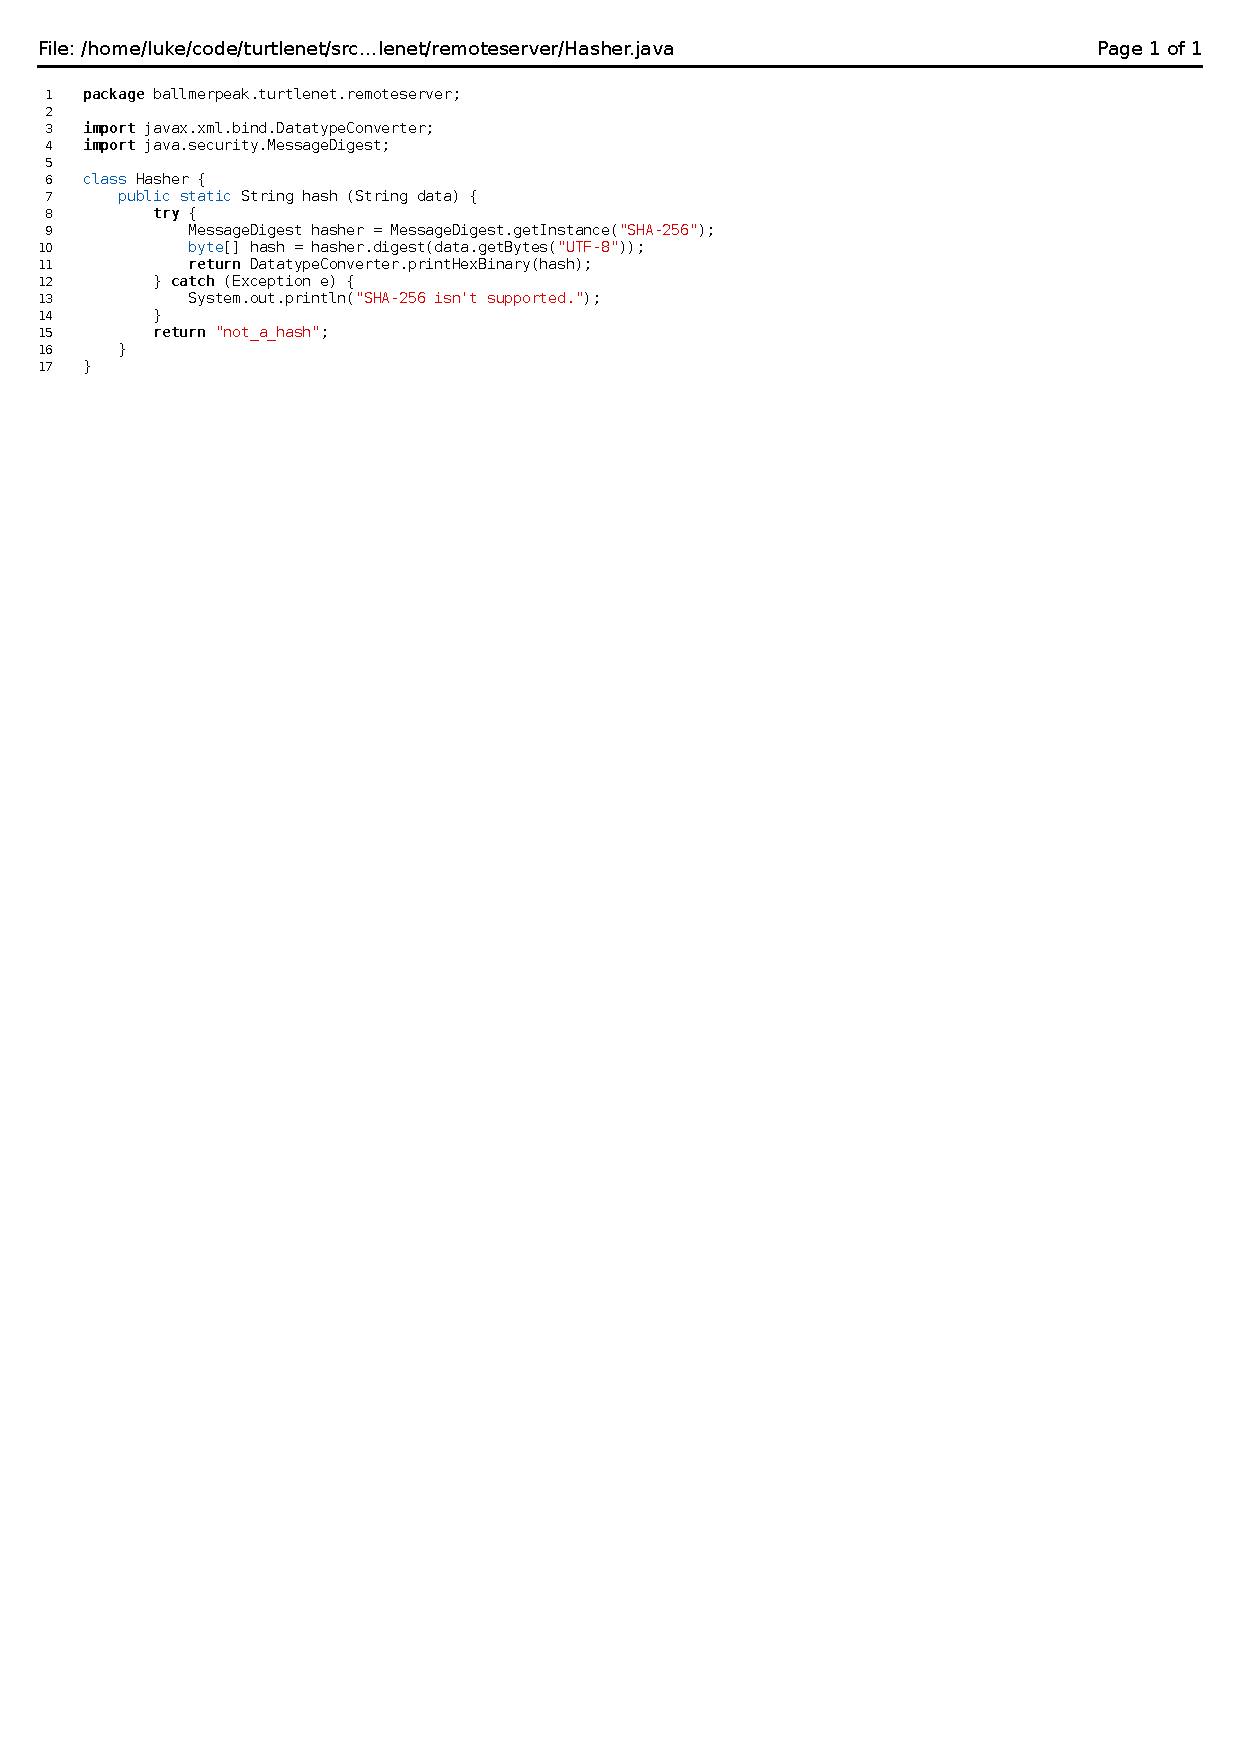
\includepdf[pages={-}]{./text/appendicies/source/23Hasher.pdf}

\chapter{Deadlines}
\begin{itemize}
\item \textbf{2014-01-31} topic and team
\item \textbf{2014-02-14} requirements
\item \textbf{2014-03-14} design
\item \textbf{2014-05-09} portfolio \& individual submission
\end{itemize}

\chapter{Licence}
Ballmer Peak (i.e.: The students which worked on Turtlenet) have waived their
rights via the CC0 licence. The university of liverpool now has sole claim
to limiting rights placed upon Turtlenet (NB: Not sole rights to it, the effect
of the CC0 waiver is to grant all the rights we had to everyone. The limitations
placed upon Turtlenet by The University Of Liverpool now apply to any user of
Turtlenet to the same extent they did to us before the waiver.).
\label{licence}
\begin{figure}[h]
    \centering
    
\includegraphics{images/appendicies/licence.png}
\end{figure}

\begin{center}
To the extent possible under law, Ballmer Peak has waived all copyright and
related or neighboring rights to Turtlenet and Associated Documentation. This
work is published from: United Kingdom.
\end{center}

\section {Statement of Purpose}
The laws of most jurisdictions throughout the world automatically confer
exclusive Copyright and Related Rights (defined below) upon the creator and
subsequent owner(s) (each and all, an "owner") of an original work of authorship
and/or a database (each, a "Work").

Certain owners wish to permanently relinquish those rights to a Work for the
purpose of contributing to a commons of creative, cultural and scientific works
("Commons") that the public can reliably and without fear of later claims of
infringement build upon, modify, incorporate in other works, reuse and
redistribute as freely as possible in any form whatsoever and for any purposes,
including without limitation commercial purposes. These owners may contribute to
the Commons to promote the ideal of a free culture and the further production of
creative, cultural and scientific works, or to gain reputation or greater
distribution for their Work in part through the use and efforts of others.

For these and/or other purposes and motivations, and without any expectation of
additional consideration or compensation, the person associating CC0 with a Work
(the "Affirmer"), to the extent that he or she is an owner of Copyright and
Related Rights in the Work, voluntarily elects to apply CC0 to the Work and
publicly distribute the Work under its terms, with knowledge of his or her
Copyright and Related Rights in the Work and the meaning and intended legal
effect of CC0 on those rights.

\section{Copyright and Related Rights}
A Work made available under CC0 may be protected by copyright and related or
neighboring rights ("Copyright and Related Rights"). Copyright and Related
Rights include, but are not limited to, the following:

\begin{enumerate}
\item the right to reproduce, adapt, distribute, perform, display, communicate,
      and translate a Work;
\item moral rights retained by the original author(s) and/or performer(s);
\item publicity and privacy rights pertaining to a person's image or likeness
      depicted in a Work;
\item rights protecting against unfair competition in regards to a Work, subject
      to the limitations in paragraph 4(a), below;
\item rights protecting the extraction, dissemination, use and reuse of data in
      a Work;
\item database rights (such as those arising under Directive 96/9/EC of the
      European Parliament and of the Council of 11 March 1996 on the legal
      protection of databases, and under any national implementation thereof,
      including any amended or successor version of such directive); and
\item other similar, equivalent or corresponding rights throughout the world
      based on applicable law or treaty, and any national implementations
      thereof.
\end{enumerate}

\section{Waiver}
To the greatest extent permitted by, but not in contravention of, applicable
law, Affirmer hereby overtly, fully, permanently, irrevocably and
unconditionally waives, abandons, and surrenders all of Affirmer's Copyright and
Related Rights and associated claims and causes of action, whether now known or
unknown (including existing as well as future claims and causes of action), in 
the Work (i) in all territories worldwide, (ii) for the maximum duration
provided by applicable law or treaty (including future time extensions),
(iii) in any current or future medium and for any number of copies, and (iv) for
any purpose whatsoever, including without limitation commercial, advertising or
promotional purposes (the "Waiver"). Affirmer makes the Waiver for the benefit
of each member of the public at large and to the detriment of Affirmer's heirs
and successors, fully intending that such Waiver shall not be subject to
revocation, rescission, cancellation, termination, or any other legal or
equitable action to disrupt the quiet enjoyment of the Work by the public as
contemplated by Affirmer's express Statement of Purpose.

\section{Public License Fallback}
Should any part of the Waiver for any reason be judged legally invalid or
ineffective under applicable law, then the Waiver shall be preserved to the
maximum extent permitted taking into account Affirmer's express Statement of
Purpose. In addition, to the extent the Waiver is so judged Affirmer hereby
grants to each affected person a royalty-free, non transferable, non
sublicensable, non exclusive, irrevocable and unconditional license to exercise
Affirmer's Copyright and Related Rights in the Work (i) in all territories
worldwide, (ii) for the maximum duration provided by applicable law or treaty
(including future time extensions), (iii) in any current or future medium and
for any number of copies, and (iv) for any purpose whatsoever, including without
limitation commercial, advertising or promotional purposes (the "License"). The
License shall be deemed effective as of the date CC0 was applied by Affirmer to
the Work. Should any part of the License for any reason be judged legally
invalid or ineffective under applicable law, such partial invalidity or
ineffectiveness shall not invalidate the remainder of the License, and in such
case Affirmer hereby affirms that he or she will not (i) exercise any of his or
her remaining Copyright and Related Rights in the Work or (ii) assert any
associated claims and causes of action with respect to the Work, in either case
contrary to Affirmer's express Statement of Purpose.

\section{Limitations and Disclaimers}
\begin{enumerate}
\item No trademark or patent rights held by Affirmer are waived, abandoned,
      surrendered, licensed or otherwise affected by this document.
\item Affirmer offers the Work as-is and makes no representations or warranties
      of any kind concerning the Work, express, implied, statutory or otherwise,
      including without limitation warranties of title, merchantability, fitness
      for a particular purpose, non infringement, or the absence of latent or
      other defects, accuracy, or the present or absence of errors, whether or
      not discoverable, all to the greatest extent permissible under applicable
      law.
\item Affirmer disclaims responsibility for clearing rights of other persons
      that may apply to the Work or any use thereof, including without
      limitation any person's Copyright and Related Rights in the Work. Further,
      Affirmer disclaims responsibility for obtaining any necessary consents,
      permissions or other rights required for any use of the Work.
\item Affirmer understands and acknowledges that Creative Commons is not a party
      to this document and has no duty or obligation with respect to this CC0 or
      use of the Work.
\end{enumerate}

\section{Limitations places upon Turtlenet by The University of Liverpool}

\includepdf[pages={-}]{./text/appendicies/ip-policy.pdf}
\section{Included Works}
We did not write or create the following:
\begin{itemize}
\item writeup/latex/tikz-uml.sty
\item writeup/latex/todonotes.sty
\item writeup/latex/ulem.sty
\item writeup/images/appendicies/licence.png (CC0 licence logo)
\item The CC0 licence text
\item client/web\_interface\_mockup/jquery.js \todo{look into legality of distribution}
\item client/web\_interface\_mockup/turtles.ttf \todo{look into legality of distribution}
\end{itemize}


\chapter{TODO}
\section{General}
Errors shouldn't just display a message, they should be properly handled
Get a real DB\\
REVOKE claims and messages after a certain date if private key leaked\\
escape backslashes in message content\\
chang all references to ascii text to UTF-8 text\\

\section{Requirements \textbf{Weeks 1-3}}
1. Project Desc.
\begin{itemize}
\item \textbf{COMPLETE} Project being done for (Peter)
\item \textbf{COMPLETE} Mission Statement (Luke)
\item \textbf{COMPLETE} Mission Objective (Luke)
\item \textbf{COMPLETE} Threat Model (Luke)
\end{itemize}

2. Statement of Deliverables
\begin{itemize}
\item \textbf{COMPLETE}    Desc. of anticipated documentation (Luke)
\item \textbf{COMPLETE}    Desc. of anticipated software (Aishah)
\item \textbf{COMPLETE}    Desc. + Eval. of any anticipated experiments + blackbox (Louis)
\item \textbf{COMPLETE}    User view and requirements (Luke)
\item \textbf{COMPLETE}    System requirements (Luke)
\item \textbf{COMPLETE}    Transaction requirements (Aishah)
\end{itemize}

3. Project and Plan
\begin{itemize}
\item \textbf{COMPLETE}    Facebook research (Leon)
\item \textbf{COMPLETE}    Case Study: Tor (Luke)
\item \textbf{COMPLETE}    Case Study: alt.anonymous.messages and mix networks (Luke)
\item \textbf{COMPLETE}    Case Study: PGP and E-Mail (Luke)
\item \textbf{COMPLETE}    Implementation Stage (Peter)
\item \textbf{COMPLETE}    Milestone Identification (Milestones can most easily be recognised as deliverables) (Mike)
\item \textbf{COMPLETE}    Gantt Chart (Mike)
\item \textbf{COMPLETE}    Risk Assessment (Mike)
\end{itemize}

4. Bibliography
\begin{itemize}
\item \textbf{COMPLETE} Bibliography framework (Luke)
\item \textbf{COMPLETE} Add citations where relevent (Everyone, in their own sections)
\end{itemize}

\section{Design \textbf{Weeks 4-X}}
\begin{itemize}
\item \textbf{DRAFTED}    Use Case Diagram (Mike)
\item \textbf{DRAFTED}    Data Dictionary (Mike)
\item \textbf{DRAFTED}    Mobile GUI Design (Leon)
\item \textbf{DRAFTED}    Sequence Diagram (Leon)
\item \textbf{DRAFTED}    HTML GUI Design (Louis)
\item \textbf{DRAFTED}    DB Design (Aishah)
\item \textbf{INCOMPLETE}    Transaction Design (Aishah) (what values each transaction modifies)
\item \textbf{DRAFTED}    Server GUI Design (Peter)
\item \textbf{DRAFTED}    Class Interfaces (Luke)
\item \textbf{DRAFTED}    Protocol (Luke)
\item \textbf{DRAFTED}    Architecture (Luke)
\item \textbf{DRAFTED}    Data Flow Diagrams (Luke)
\item \textbf{NOT IN PDF}    Pseudocode (Luke)
\item \textbf{INCOMPLETE}    Class Diagram (???)
\end{itemize}

\chapter{\sout{Bugs} Accidental Features}
\begin{itemize}
\item Entering the wrong password erases the database.
\end{itemize}

\end{appendices}

\listoftodos
\todototoc

\printbibliography

\end{document}
